\documentclass[9pt]{IEEEtran}

\usepackage[T1]{fontenc}
\usepackage{lmodern}
\usepackage{amssymb,amsmath}
\usepackage{ifxetex,ifluatex}




\usepackage{fixltx2e} % provides \textsubscript
% use upquote if available, for straight quotes in verbatim environments
\IfFileExists{upquote.sty}{\usepackage{upquote}}{}
\ifnum 0\ifxetex 1\fi\ifluatex 1\fi=0 % if pdftex
  \usepackage[utf8]{inputenc}
\else % if luatex or xelatex
  \ifxetex
    \usepackage{mathspec}
    \usepackage{xltxtra,xunicode}
  \else
    \usepackage{fontspec}
  \fi
  \defaultfontfeatures{Mapping=tex-text,Scale=MatchLowercase}
  \newcommand{\euro}{€}
\fi
% use microtype if available
\IfFileExists{microtype.sty}{\usepackage{microtype}}{}
\ifxetex
  \usepackage[setpagesize=false, % page size defined by xetex
              unicode=false, % unicode breaks when used with xetex
              xetex]{hyperref}
\else
  \usepackage[unicode=true]{hyperref}
\fi
\hypersetup{breaklinks=true,
            bookmarks=true,
            pdfauthor={},
            pdftitle={Taming math and physics using SymPy},
            colorlinks=true,
            citecolor=blue,
            urlcolor=black,
            linkcolor=magenta,
            pdfborder={0 0 0}}
\urlstyle{same}  % don't use monospace font for urls
\setlength{\parindent}{0pt}
\setlength{\parskip}{6pt plus 2pt minus 1pt}
\setlength{\emergencystretch}{3em}  % prevent overfull lines
\setcounter{secnumdepth}{0}

\usepackage{etoolbox}


\title{{\Huge Taming math and physics using \texttt{SymPy} }}
%	A tale of with equations and code}
%\author{Ivan Savov}
\author{{\normalsize Tutorial based on the \href{http://minireference.com}{{\sc No bullshit guide}} series of textbooks by \href{mailto:ivan.savov+SYMPYTUT@gmail.com}{Ivan Savov}}}
\date{\today}

%\usepackage{listings}
\usepackage{moreverb}
\usepackage[letterpaper,bmargin=1.1cm,rmargin=0.95cm,lmargin=0.95cm,tmargin=1cm,headsep=0.2cm,footskip=0.5cm]{geometry}


\usepackage{bbm}
\usepackage{wrapfig}
\usepackage{graphicx}

\usepackage{ifthen}

\newboolean{TUTORIAL}				% if TUTORIAL==true:
\setboolean{TUTORIAL}{true}			%     show extra defs and repeats of explanations 

\newboolean{FORLA}				% if FORLA:  show extra content for LA book
\setboolean{FORLA}{true}			% if not FORLA:  show content for MathPhys book


\newcommand{\printcp}{}
\newcommand{\printni}{}

% doest work
%\usepackage[titles]{tocloft}
%\setlength{\cftbeforechapskip}{.1ex}
%\setlength{\cftbeforesecskip}{-.5ex}

\setcounter{secnumdepth}{1}
\setcounter{tocdepth}{0}
\usepackage{setspace}
%\addtocontents{toc}{\protect\setstretch{-20.1}}

\newcommand*{\eqdef}{\stackrel{\raisebox{-2pt}{\scalebox{0.48}{def}}}{=}}   % "defined to be equal" symbol (prev. used \equiv; other common is := )

\begin{document}


\makeatletter
\preto{\@verbatim}{\topsep=0pt \partopsep=0pt \vspace{-1.2mm}}
\makeatother



        \maketitle

%\vspace{-2mm}

\begin{abstract}
Most people consider math and physics to be scary beasts from which it is best to keep one's distance.
Computers, however, can help us tame the complexity and tedious arithmetic manipulations associated with these subjects.
Indeed, math and physics are much more approachable once you have the power of computers on your side.
%
%Understand math and physics

This tutorial serves a dual purpose.
On one hand, it serves as a review of the fundamental concepts of mathematics for computer-literate people.
%who may have forgotten their math or never quite learned it detail.
On the other hand, this tutorial serves to demonstrate to students how a computer algebra system 
can help them with their classwork.
A word of warning is in order.
Please don't use \texttt{SymPy} to avoid the suffering associated with your homework!
Teachers assign homework problems to you
%not because they want you to suffer but 
because they want you to learn.
Do your homework by hand,
but if you want, you can check your answers using \texttt{SymPy}.
Better yet, use \texttt{SymPy} to invent extra practice problems for yourself.
%
%Let's get started!

%The whole point of homework is for you to suffer.
%Mathematical skill is developed through mathematical suffering---only 
%when trying to solve a problem that you haven't solved before will you 
%be forced to think and practice your skills.
%Do not use \texttt{SymPy} to cheat on your homework! 
%You can use \texttt{SymPy} to check your answers though.
%In fact, one of the best ways to learn math is to 
% solve them by hand, and then check your answers using \texttt{sympy}.

%Let's kick some mathematical ass!

\end{abstract}

\begin{spacing}{-1}
\tableofcontents
\end{spacing}

%!TEX root = noBSguideMathMechCalc.tex

%%!TEX root = noBSguideMathMechCalc.tex

%%!TEX root = noBSguideMathMechCalc.tex

%\input{99.sympy_tutorial.tex}
%%%%%%%%%%%%%%%%%%%%%%%%%%%%%%%%%%%%%%%%%%%%%%%%%%%%%%%%%%%%%%%%%




\ifthenelse{\boolean{TUTORIAL}}{}{

\vspace*{-5mm}

	Computers can be very useful for dealing with complicated math expressions
	or when slogging through tedious calculations.	
	Throughout this book we used \texttt{SymPy} to illustrate several concepts from math and physics.
	%	to illustrate how computers can help us manipulate math and physics objects 
	We'll now review all the math and physics tools available through the \texttt{SymPy} command line.
	Don't worry if you're not a computer person;
	we'll only discuss concepts we covered in the book,
	and the computer commands we'll learn are very similar to the math operations you're already familiar with.
	This section also serves as a final review of the material covered in the book.
} 


%=======================================================================  introduction
\section*{Introduction}
% \label{sec:sympytut_introduction}

You can use a computer algebra system (CAS) to compute complicated math expressions,
solve equations,
perform calculus procedures,
and simulate physics systems.

All computer algebra systems offer essentially the same functionality,
so it doesn't matter which system you use: 
there are free systems like \texttt{SymPy}, \texttt{Magma}, or \texttt{Octave}, 
and commercial systems like \texttt{Maple}, \texttt{MATLAB}, and \texttt{Mathematica}.
This tutorial is an introduction to \texttt{SymPy},
which is a \emph{symbolic} computer algebra system written in the programming language \texttt{Python}. 
In a symbolic CAS, 
numbers and operations are represented symbolically, so the answers obtained are exact.
For example, the number $\sqrt{2}$ is represented in \texttt{SymPy} as the object \texttt{Pow(2,1/2)},
whereas in \emph{numerical} computer algebra systems like \texttt{Octave}, the number $\sqrt{2}$ is 
represented as the approximation $1.41421356237310$ (a \texttt{float}).
For most purposes the approximation is okay,
but sometimes approximations can lead to problems:
\texttt{float(sqrt(2))*float(sqrt(2)) = 2.00000000000000044} $\neq 2$.
Because \texttt{SymPy} uses exact representations, 
you'll never run into such problems: \texttt{Pow(2,1/2)*Pow(2,1/2)}$ = 2$.


\ifthenelse{\boolean{TUTORIAL}}{
This tutorial is organized as follows.
We'll begin by introducing the \texttt{SymPy} basics and the bread-and-butter functions
used for manipulating expressions and solving equations.
Afterward, we'll discuss the \texttt{SymPy} functions that implement calculus operations like differentiation and integration.
We'll also introduce the functions used to deal with vectors and complex numbers.
Later we'll see how to use vectors and integrals to understand Newtonian mechanics.
\ifthenelse{\boolean{FORLA}}
	{In the last section, we'll introduce the linear algebra functions available in \texttt{SymPy}.}
	{}
}{}


This tutorial presents many explanations as blocks of code. 
Be sure to try the code examples on your own by typing the commands into \texttt{SymPy}.
It's always important to verify for yourself!
%Don't be a passive reader: 
%type out the commands presented. 


%\vspace{1cm}	% to push REPL at top of col2

%=======================================================================  using_sympy
\section*{Using SymPy}
% \label{sec:sympytut_using_sympy}

The easiest way to use \texttt{SymPy},
provided you're connected to the internet,
is to visit \href{http://live.sympy.org}{\texttt{http://live.sympy.org}}.
You'll be presented with an interactive prompt into which
you can enter your commands---right in your browser. 

If you want to use \texttt{SymPy} on your own computer,
you must install \texttt{Python} and the python package \texttt{sympy}.
You can then open a command prompt and start a \texttt{SymPy} session using:



\small
\begin{verbatimtab}
you@host$ python
Python X.Y.Z 
[GCC a.b.c (Build Info)] on platform
Type "help", "copyright", or "license" for more information.
>>> from sympy import *
>>> 
\end{verbatimtab}
\normalsize

\noindent
The \texttt{>{}>{}>} prompt indicates you're in the \texttt{Python} shell which accepts \texttt{Python} commands.
The command \texttt{from sympy import *}$\;$ imports all the \texttt{SymPy} functions into the current namespace. 
All \texttt{SymPy} functions are now available to you.
%
To exit the python shell press \texttt{CTRL+D}. 
%
%\small
%\begin{verbatimtab}
%>>>  ( press CTRL + D )
%you@host$  
%\end{verbatimtab}
%\normalsize

I highly recommend you also install \texttt{ipython},
which is an improved interactive python shell.
If you have \texttt{ipython} and \texttt{SymPy} installed,
you can start an \texttt{ipython} shell with \texttt{SymPy} pre-imported using the command \texttt{isympy}.
For an even better experience,
you can try \texttt{jupyter notebook},
which is a web frontend for the \texttt{ipython} shell.

Each section \ifthenelse{\boolean{TUTORIAL}}{of this tutorial}{in this appendix} begins with a python \texttt{import} statement
for the functions used in that section.
If you use the statement \texttt{from sympy import *}\,\, in the beginning of your code,
you don't need to run these individual import statements,
but I've included them so you'll know which 
\texttt{SymPy} vocabulary is covered in each section.





%
\ifthenelse{\boolean{TUTORIAL}}{
\def\lesection{\section}
}{
\def\lesection{\section*}
}

%=======================================================================  basics
\lesection{Fundamentals of mathematics}
\label{sec:sympytut_fundamentals_of_mathematics}

Let's begin by learning about the basic \texttt{SymPy} objects and the operations we can carry out on them. 
We'll learn the \texttt{SymPy} equivalents of 
\ifthenelse{\boolean{TUTORIAL}}{many math verbs like}{the math verbs we used in Chapter~1:} 
``to solve'' (an equation),  
%``to simplify'' (an expression), 
``to expand'' (an expression), 
``to factor'' (a polynomial).

\subsection{Numbers}
\label{basics:numbers}

\small
\begin{verbatimtab}
>>> from sympy import  sympify, S,  evalf, N
\end{verbatimtab}
\normalsize

\noindent
In \texttt{Python}, there are two types of number objects: \texttt{int}s and \texttt{float}s.%

\small
\begin{verbatimtab}
>>> 3
3                             # an int
>>> 3.0
3.0                           # a float 
\end{verbatimtab}
\normalsize
Integer objects in \texttt{Python} are a faithful representation of the set of integers $\mathbb{Z}=\{\ldots,-2,-1,0,1,2,\ldots\}$.
Floating point numbers are approximate representations of the reals $\mathbb{R}$.
%The name ``floating point'' comes from the fact that \texttt{float}s can represent very small numbers 
%and very large numbers (by moving the decimal point).
Regardless of its absolute size, 
a floating point number is only accurate to 16 decimals.
% you can think of floats as rational numbers of the form $\frac{m}{10^n}$ where $m<10^{16}$ and $< n <$.

%We won't go any further into the implementation details of how numbers are represented;
%I just wanted to point out the difference between \texttt{int}s, \texttt{float}s, 
%and the set of real numbers $\mathbb{R}$. 
%Sandy said: these lines could be more fitting for a teacher's guide, but I think for students it is TMI, since the differences are explained concisely and neatly above.


% Floats are only approximations, but if you want to do calculations with floats you can use the GPU
 
Special care is required when specifying rational numbers,
because integer division might not produce the answer you want.
In other words, 
\texttt{Python} will not automatically convert the answer to a floating point number,
but instead round the answer to the closest integer:
\small
\begin{verbatimtab}
>>> 1/7
0                             # int/int gives int 
\end{verbatimtab}
\normalsize

\noindent
To avoid this problem, you can force \texttt{float} division by using the number \texttt{1.0} instead of \texttt{1}:
\small
\begin{verbatimtab}
>>> 1.0/7
0.14285714285714285           # float/int gives float
\end{verbatimtab}
\normalsize

\noindent
This result is better, but it's still only an approximation of the exact number $\frac{1}{7} \in \mathbb{Q}$, 					\index{fraction}
since a \texttt{float} has 16 decimals while the decimal expansion of $\frac{1}{7}$ is infinitely long. 
To obtain an \emph{exact} representation of $\frac{1}{7}$ you need to create a \texttt{SymPy} expression.
You can \texttt{sympify} any expression using the shortcut function \texttt{S()}:
\small
\begin{verbatimtab}
S('1/7')
1/7                           # = Rational(1,7)
\end{verbatimtab}
\normalsize

\noindent
Note the input to \texttt{S()} is specified as a text string delimited by quotes.
We could have achieved the same result using \texttt{S('1')/7} since
a \texttt{SymPy} object divided by an \texttt{int} is a \texttt{SymPy} object.

Except for the tricky \texttt{Python} division operator, 
other math operators like addition \texttt{+}, subtraction \texttt{-}, 
and multiplication \texttt{*} work as you would expect.
The syntax \texttt{**} is used in \texttt{Python} to denote exponentiation:											\index{exponent}
\small
\begin{verbatimtab}
>>> 2**10                    # same as S('2^10')
1024
\end{verbatimtab}
\normalsize

\noindent
When solving math problems, 
it's best to work with \texttt{SymPy} objects,
and wait to compute the numeric answer in the end.
To obtain a numeric approximation of a \texttt{SymPy} object as a  \texttt{float}, 
call  its \texttt{.evalf()} method: %Sandy said: what do you mean by 'call'?

\small
\begin{verbatimtab}
>>> pi
pi
>>> pi.evalf()
3.14159265358979
\end{verbatimtab}
\normalsize

\noindent
The method \texttt{.n()} is equivalent to \texttt{.evalf()}.
The global \texttt{SymPy} function \texttt{N()} can also be used to to compute numerical values.
%
You can easily change the number of digits of precision of the approximation.										\index{precision}
Enter \texttt{pi.n(400)} to obtain an approximation of $\pi$ to 400 decimals.

\subsection{Symbols}
\label{basics:symbols}

\small
\begin{verbatimtab}
>>> from sympy import Symbol, symbols
\end{verbatimtab}
\normalsize

\noindent
Python is a civilized language so there's no need to define variables before assigning values to them.
When you write \texttt{a = 3}, you define a new name \texttt{a} and set it to the value \texttt{3}.
You can now use the name \texttt{a} in  subsequent calculations.

Most interesting \texttt{SymPy} calculations require us to define \texttt{symbols},
which are the \texttt{SymPy} objects for representing variables and unknowns.
For your convenience, when \href{http://live.sympy.org}{\texttt{live.sympy.org}} starts,
it runs the following commands automatically:

\small
\begin{verbatimtab}
>>> from __future__ import division
>>> from sympy import *
>>> x, y, z, t = symbols('x y z t')
>>> k, m, n = symbols('k m n', integer=True)
>>> f, g, h = symbols('f g h', cls=Function)
\end{verbatimtab}
\normalsize

\noindent
The first statement instructs python to convert \texttt{1/7} to \texttt{1.0/7} when dividing,
potentially saving you from any \texttt{int} division confusion.
The second statement imports all the \texttt{SymPy} functions.
The remaining statements define some generic symbols \texttt{x}, \texttt{y}, \texttt{z}, and \texttt{t},
and several other symbols with special properties.

Note the difference between the following two statements:

\small
\begin{verbatimtab}
>>> x + 2           
x + 2                 # an Add expression
>>> p + 2 
NameError: name 'p' is not defined
\end{verbatimtab}
\normalsize

\noindent
The name \texttt{x} is defined as a symbol, so \texttt{SymPy} knows that \texttt{x + 2} is an expression;
but the variable \texttt{p} is not defined, so \texttt{SymPy} doesn't know what to make of \texttt{p + 2}.
To use \texttt{p} in expressions, 
you must first define it as a symbol:

\small
\begin{verbatimtab}
>>> p = Symbol('p')   # the same as p = symbols('p')
>>> p + 2
p + 2                 # = Add(Symbol('p'), Integer(2))
\end{verbatimtab}
\normalsize


\printcp

\noindent
You can define a sequence of variables using the following notation:
\small
\begin{verbatimtab}
>>> a0, a1, a2, a3 = symbols('a0:4')
\end{verbatimtab}
\normalsize

\noindent
You can use any name you want for a variable,
but it's best if you avoid the letters \texttt{Q,C,O,S,I,N} and \texttt{E} because they have special uses in \texttt{SymPy}:
\texttt{I} is the unit imaginary number $i\equiv\sqrt{-1}$, 
\texttt{E} is the base of the natural logarithm,
\texttt{S()} is the \texttt{sympify} function,
\texttt{N()} is used to obtain numeric approximations, and
\texttt{O} is used for big-\texttt{O} notation.

The underscore symbol \texttt{\char`_} is a special variable that contains the result of the last printed value.
The variable \texttt{\char`_} is analogous to the \texttt{ans} button on certain calculators,
and is useful in multi-step calculations:

\small
\begin{verbatimtab}
>>> 3+3
6
>>> _*2
12
\end{verbatimtab}
\normalsize


\subsection{Expressions}
\label{basics:expressions}

\small
\begin{verbatimtab}
>>> from sympy import simplify, factor, expand, collect
\end{verbatimtab}
\normalsize

\noindent
You define \texttt{SymPy} expressions by combining symbols with basic math operations and other functions: 

\small
\begin{verbatimtab}
>>> expr = 2*x + 3*x - sin(x) - 3*x + 42
>>> simplify(expr)
2*x - sin(x) + 42
\end{verbatimtab}
\normalsize

\noindent
The function \texttt{simplify} can be used on any expression to simplify it.
The examples below illustrate other useful \texttt{SymPy} functions
that correspond to common mathematical operations on expressions: 
%COMMENT: do you mean 'or' expressions? @SANDY: no, operations like factor, expand, etc, act  on math expressions

																								\index{factoring} \index{expand} \index{collect}

\small
\begin{verbatimtab}
>>> factor( x**2-2*x-8 )
(x - 4)*(x + 2)
>>> expand( (x-4)*(x+2) )
x**2 - 2*x - 8
>>> collect(x**2 + x*b + a*x + a*b, x)
x**2 + (a+b)*x + a*b     # collect terms for diff. pows of x 
\end{verbatimtab}
\normalsize

\noindent
To substitute a given value into an expression,																\index{substitution}
call the \texttt{.subs()} method, passing in a python dictionary object \texttt{\{ key:val, ... \}} 
with the symbol--value substitutions you want to make:

\small
\begin{verbatimtab}
>>> expr  = sin(x) + cos(y)
>>> expr
sin(x) + cos(y)
>>> expr.subs({x:1, y:2})
sin(1) + cos(2)
>>> expr.subs({x:1, y:2}).n()
0.425324148260754
\end{verbatimtab}
\normalsize

\noindent
Note how we used \texttt{.n()} to obtain the expression's numeric value.

\subsection{Solving equations}
\label{basics:solving_equations}

\small
\begin{verbatimtab}
>>> from sympy import solve
\end{verbatimtab}
\normalsize

\noindent
The function \texttt{solve} is the main workhorse in \texttt{SymPy}. 
This incredibly powerful function knows how to solve all kinds of equations.
In fact \texttt{solve} can solve pretty much \emph{any} equation!
When high school students learn about this function, they get really angry---why 
did they spend five years of their life learning to solve various equations by hand,
when all along there was this \texttt{solve} thing that could do all the math for them?
%Computers are nice like that.
Don't worry, learning math is \emph{never} a waste of time.


The function \texttt{solve} takes two arguments.
Use \texttt{solve(expr,var)} to solve the equation \texttt{expr==0} for the variable \texttt{var}.
%you want to solve assuming the form 
%The first argument specifies an expression which is equal to zero, 
You can rewrite any equation in the form \texttt{expr==0} by moving all the terms to one side of the equation;
the solutions to $A(x)=B(x)$ are the same as the solutions to $A(x)-B(x)=0$.

For example, 
to solve the quadratic equation $x^2+2x-8=0$, use

\small
\begin{verbatimtab}
>>> solve( x**2 + 2*x - 8, x)
[2, -4]
\end{verbatimtab}
\normalsize

\noindent
In this case the equation has two solutions so \texttt{solve} returns a list.
Check that $x=2$ and $x=-4$ satisfy the equation $x^2+2x-8=0$.

The best part about \texttt{solve} and \texttt{SymPy} is that you can obtain symbolic answers when solving equations. 
Instead of solving one specific quadratic equation,
we can solve all possible equations of the form $ax^2 + bx+c=0$ using the following steps:

\small
\begin{verbatimtab}
>>> a, b, c = symbols('a b c')
>>> solve( a*x**2 + b*x + c, x)
[(-b + sqrt(b**2 - 4*a*c))/(2*a), (-b-sqrt(b**2-4*a*c))/(2*a)]
\end{verbatimtab}
\normalsize

\noindent
In this case \texttt{solve} calculated the solution in terms of the symbols \texttt{a}, \texttt{b}, and \texttt{c}.
You should be able to recognize the expressions in the solution---it's the quadratic formula $x_{1,2} = \frac{-b \pm \sqrt{b^2 - 4ac}}{2a}$.

\ifthenelse{\boolean{TUTORIAL}}{  
	\input{99.quadratic_eqn_subsitution_example.tex}
}{} 


\bigskip

\noindent
To solve a \emph{system of equations},
you can feed \texttt{solve} with the list of equations as the first argument, and specify the list of unknowns you want to solve for as the second argument.
For example, to solve for $x$ and $y$ in the system of equations $x+y=3$ and $3x-2y=0$, use

\small
\begin{verbatimtab}
>>> solve([x + y - 3, 3*x - 2*y], [x, y])
{x: 6/5, y: 9/5}
\end{verbatimtab}
\normalsize

\bigskip

\noindent
The function \texttt{solve} is like a Swiss Army knife you can use to solve all kind of problems.
Suppose you want to \emph{complete the square} in the expression $x^2-4x+7$,								\index{completing the square}
that is, you want to find constants $h$ and $k$ such that $x^2-4x+7 = (x-h)^2 +k$.
There is no special ``complete the square'' function in \texttt{SymPy},
but you can call \texttt{solve} on the equation $(x-h)^2 +k \ - \  (x^2-4x+7) = 0$
to find the unknowns $h$ and $k$:

\small
\begin{verbatimtab}
>>> h, k = symbols('h k')
>>> solve( (x-h)**2 + k  - (x**2-4*x+7), [h,k] )
[(2, 3)]                               # so h = 2 and k = 3
>>> ((x-2)**2+3).expand()              # verify...
x**2 - 4*x + 7
\end{verbatimtab}
\normalsize

\noindent
Learn the basic \texttt{SymPy} commands 
and you'll never need to suffer another tedious arithmetic calculation painstakingly performed by hand again!



\subsection{Rational functions}
\label{basics:rational_functions}

\small
\begin{verbatimtab}
>>> from sympy import together, apart
\end{verbatimtab}
\normalsize

\noindent
By default, \texttt{SymPy} will not combine or split rational expressions.
You need to use \texttt{together} to symbolically calculate the addition of fractions:									\index{fraction}

\small
\begin{verbatimtab}
>>> a, b, c, d = symbols('a b c d')
>>> a/b + c/d
a/b + c/d
>>> together(a/b + c/d)
(a*d + b*c)/(b*d)
\end{verbatimtab}
\normalsize

\noindent
Alternately, if you have a rational expression and want to divide the numerator by the denominator,
use the \texttt{apart} function:

\small
\begin{verbatimtab}
>>> apart( (x**2+x+4)/(x+2)  )
x - 1  +  6/(x + 2)
\end{verbatimtab}
\normalsize


\subsection{Exponentials and logarithms}
\label{basics:exponentials_and_logarithms}

																								\index{exponential} \index{logarithm}
Euler's number $e=2.71828\ldots$ is defined one of several ways,												\index{Euler's!number}
\[
  e \equiv \lim_{n\to \infty} \left( 1 + \frac{1}{n}\right)^{n}
    \equiv \lim_{\epsilon \to 0} \left( 1 + \epsilon\right)^{1/\epsilon}
    \equiv \sum_{n=0}^\infty \frac{1}{n!},
\]
and is denoted \texttt{E} in \texttt{SymPy}.
Using \texttt{exp(x)} is equivalent to \texttt{E**x}.

The functions \texttt{log} and \texttt{ln} both compute the logarithm base $e$:

\small
\begin{verbatimtab}
>>> log(E**3)    # same as ln(E**3)
3
\end{verbatimtab}
\normalsize

\noindent
By default, \texttt{SymPy} assumes the inputs to functions like \texttt{exp} and \texttt{log} are complex numbers,
so it will not expand certain logarithmic expressions.
However, indicating to \texttt{SymPy} that the inputs are positive real numbers will make the expansions work:

\small
\begin{verbatimtab}
>>> x, y = symbols('x y')
>>> log(x*y).expand()
log(x*y)
>>> a, b = symbols('a b', positive=True)
>>> log(a*b).expand()
log(a) + log(b)
\end{verbatimtab}
\normalsize
\subsection{Polynomials}
\label{basics:polynomials}

Let's define a polynomial $P$ with roots at $x=1$, $x=2$, and $x=3$:											\index{polynomial}

\small
\begin{verbatimtab}
>>> P = (x-1)*(x-2)*(x-3)
>>> P
(x - 1)*(x - 2)*(x - 3)
\end{verbatimtab}
\normalsize

\noindent
To see the expanded version of the polynomial,
call its \texttt{expand} method:																			\index{expand}

\small
\begin{verbatimtab}
>>> P.expand()
x**3 - 6*x**2 + 11*x - 6
\end{verbatimtab}
\normalsize

\noindent
When the polynomial is expressed in it's expanded form $P(x)=x^3-6^2 + 11x - 6$,
we can't immediately identify its roots.
This is why the factored form $P(x)=(x-1)(x-2)(x-3)$ is preferable.
To factor a polynomial,
call its \texttt{factor} method or \texttt{simplify} it:															\index{factoring}

\small
\begin{verbatimtab}
>>> P.factor()
(x - 1)*(x - 2)*(x - 3)
>>> P.simplify()
(x - 1)*(x - 2)*(x - 3)
\end{verbatimtab}
\normalsize

\noindent
Recall that the roots of the polynomial $P(x)$ are defined as the solutions to the equation $P(x)=0$.
We can use the \texttt{solve} function to find the roots of the polynomial:

\small
\begin{verbatimtab}
>>> roots = solve(P,x)
>>> roots
[1, 2, 3]
# let's check if P equals (x-1)(x-2)(x-3)
>>> simplify( P  -  (x-roots[0])*(x-roots[1])*(x-roots[2]) )   
0  
\end{verbatimtab}
\normalsize


\subsection{Equality checking}
\label{basics:equality_checking}

In the last example, we used the \texttt{simplify} function to check whether two expressions were equal.
This way of checking equality works because $P=Q$ if and only if $P-Q=0$.
This is the best way to check if two expressions are equal in \texttt{SymPy}
because it attempts all possible simplifications when comparing the expressions.
Below is a list of other ways to check whether two quantities are equal
with example cases where they fail:

\small
\begin{verbatimtab}
>>> p = (x-5)*(x+5)
>>> q = x**2 - 25
>>> p == q                                      # fail
False
>>> p - q == 0                                  # fail 
False
>>> simplify(p - q) == 0          
True
>>> sin(x)**2 + cos(x)**2  == 1                 # fail
False
>>> simplify( sin(x)**2 + cos(x)**2 - 1 ) == 0
True
\end{verbatimtab}
\normalsize


\subsection{Trigonometry}
\label{basics:trigonometry}

\small
\begin{verbatimtab}
from sympy import sin, cos, tan, trigsimp, expand_trig
\end{verbatimtab}
\normalsize

\noindent
The trigonometric functions \texttt{sin} and \texttt{cos} take inputs in radians: 					\index{radian} \index{sine} \index{cosine}

\small
\begin{verbatimtab}
>>> sin(pi/6)
1/2
>>> cos(pi/6)
sqrt(3)/2
\end{verbatimtab}
\normalsize

\noindent
For angles in degrees, 
you need a conversion factor of $\frac{\pi}{180}$[rad/$^\circ$]:

\small
\begin{verbatimtab}
>>> sin(30*pi/180)                 # 30 deg = pi/6 rads 
1/2
\end{verbatimtab}
\normalsize

\noindent
The inverse trigonometric functions $\sin^{-1}(x)\equiv \arcsin(x)$
and $\cos^{-1}(x)\equiv \arccos(x)$ are used as follows:

\small
\begin{verbatimtab}
>>> asin(1/2)
pi/6
>>> acos(sqrt(3)/2)
pi/6
\end{verbatimtab}
\normalsize
Recall that $\tan(x) \equiv \frac{\sin(x)}{\cos(x)}$.
The inverse function of $\tan(x)$ is $\tan^{-1}(x)\equiv \arctan(x)\equiv$ \texttt{atan(x)}



\small
\begin{verbatimtab}
>>> tan(pi/6)
1/sqrt(3)                          # = ( 1/2 )/( sqrt(3)/2 )
>>> atan( 1/sqrt(3) )
pi/6
\end{verbatimtab}
\normalsize

\noindent
The function \texttt{acos} returns angles in the range $[0,\pi]$,
while \texttt{asin} and \texttt{atan} return angles in the range $[-\frac{\pi}{2},\frac{\pi}{2}]$.


Here are some trigonometric identities that \texttt{SymPy} knows:												\index{trigonometric identities}

\small
\begin{verbatimtab}
>>> sin(x) == cos(x - pi/2)      
True
>>> simplify( sin(x)*cos(y)+cos(x)*sin(y) )
sin(x + y)
>>> e = 2*sin(x)**2 + 2*cos(x)**2
>>> trigsimp(e)
2
>>> trigsimp(log(e))
log(2*sin(x)**2 + 2*cos(x)**2)
>>> trigsimp(log(e), deep=True)
log(2)
\end{verbatimtab}
\normalsize

\small
\begin{verbatimtab}
>>> simplify(sin(x)**4 - 2*cos(x)**2*sin(x)**2 + cos(x)**4)
cos(4*x)/2 + 1/2
\end{verbatimtab}
\normalsize

\noindent
The function \texttt{trigsimp} does essentially the same job as \texttt{simplify}.

If instead of simplifying you want to expand a trig expression,
you should use \texttt{expand\_trig}, because the default \texttt{expand} won't touch trig functions:

\small
\begin{verbatimtab}
>>> expand(sin(2*x))        # = (sin(2*x)).expand()
sin(2*x)
>>> expand_trig(sin(2*x))   # = (sin(2*x)).expand(trig=True)
2*sin(x)*cos(x)
\end{verbatimtab}
\normalsize



\ifthenelse{\boolean{TUTORIAL}}{
	\input{99.hyperbolic_functions_sympy_tutorial.tex}

}{}



%=======================================================================  complex_numbers
\lesection{Complex numbers}
\label{sec:sympytut_complex_numbers}
																							\index{complex number}
\small
\begin{verbatimtab}
>>> from sympy import I, re, im, Abs, arg, conjugate
\end{verbatimtab}
\normalsize

\ifthenelse{\boolean{TUTORIAL}}{
	Ever since Newton,
	the word ``number'' has been used to refer to one of the following types of math objects:
	the naturals $\mathbb{N}$, 
	the integers $\mathbb{Z}$, 
	the rationals $\mathbb{Q}$, 
	and the real numbers $\mathbb{R}$.
	Each set of numbers is associated with a different class of equations.
	The natural numbers $\mathbb{N}$ appear as solutions of the equation $m+n=x$, 
	where $m$ and $n$ are natural numbers (denoted $m,n \in \mathbb{N}$).
	The integers $\mathbb{Z}$ are the solutions to equations of the form $x+m=~n$, where $m,n \in \mathbb{N}$.
	The rational numbers $\mathbb{Q}$ are necessary to solve for $x$ in $mx=n$, with $m,n \in \mathbb{Z}$.
	The solutions to $x^2=2$ are irrational (so $\notin \mathbb{Q}$) so we need an even larger set that 
	contains \emph{all} possible numbers: real set of numbers $\mathbb{R}$.
	A pattern emerges where more complicated equations require the invention of new types of numbers.

}{\noindent}% 
Consider the quadratic equation $x^2=-1$.
There are no real solutions to this equation,
but we can define an imaginary number $i =\sqrt{-1}$ (denoted \texttt{I} in \texttt{SymPy}) that satisfies this equation:

\small
\begin{verbatimtab}
>>> I*I
-1
>>> solve( x**2 + 1 , x)
[I, -I]
\end{verbatimtab}
\normalsize

\noindent
The solutions are $x=i$ and $x=-i$,
and indeed we can verify that $i^2+1=0$ and $(-i)^2+1=0$
since $i^2=-1$.

The complex numbers $\mathbb{C}$ are defined as $\{ a+bi \,|\, a,b \in \mathbb{R} \}$.
Complex numbers contain a real part and an imaginary part:

\small
\begin{verbatimtab}
>>> z = 4 + 3*I
>>> z 
4 + 3*I
>>> re(z)
4
>>> im(z)
3 
\end{verbatimtab}
\normalsize

\noindent
The \emph{polar} representation of a complex number is $z\!\equiv\!|z|\angle\theta\!\equiv \!|z|e^{i\theta}$.
For a complex number $z=a+bi$, 
the quantity $|z|=\sqrt{a^2+b^2}$ is known as the \emph{absolute value} of $z$,				
and $\theta$ is its \emph{phase} or its \emph{argument}:

\small
\begin{verbatimtab}
>>> Abs(z)
5
>>> arg(z)
atan(3/4)
\end{verbatimtab}
\normalsize

\noindent
The complex conjugate of $z=a+bi$ is the number $\bar{z} = a-bi$:



\small
\begin{verbatimtab}
>>> conjugate( z )
4 - 3*I
\end{verbatimtab}
\normalsize

\noindent
Complex conjugation is important for computing the absolute value of $z$
($|z|\equiv\sqrt{ z\bar{z} }$) and for division by $z$ ($\frac{1}{z} \equiv \frac{\bar{z}}{|z|^2}$).

\subsection{Euler's formula}
\label{complex_numbers:euler_s_formula}
																								\index{Euler's!formula}
\small
\begin{verbatimtab}
>>> from sympy import expand, rewrite
\end{verbatimtab}
\normalsize
\href{https://en.wikipedia.org/wiki/Euler's_formula}{Euler's formula} shows an important relation 
between the exponential function $e^x$ and the trigonometric functions $\sin(x)$ and $\cos(x)$:  
\[
  e^{ix} = \cos x + i \sin x.
\]
To obtain this result in \texttt{SymPy}, you must specify that the number $x$ is real
and also tell \texttt{expand} that you're interested in complex expansions:

\small
\begin{verbatimtab}
>>> x = symbols('x', real=True)
>>> exp(I*x).expand(complex=True)
cos(x) + I*sin(x) 
>>> re( exp(I*x) ) 
cos(x)
>>> im( exp(I*x) ) 
sin(x)
\end{verbatimtab}
\normalsize

\noindent
Basically, $\cos(x)$ is the real part of $e^{ix}$,
and $\sin(x)$ is the imaginary part of $e^{ix}$.
Whaaat? 
I know it's weird,
but weird things are bound to happen when you input imaginary numbers to functions.

%	\href{https://en.wikipedia.org/wiki/Euler's_identity}{Euler's identity} is Euler's formula with $x=\pi$:  
%	$e^{i\pi} = \cos \pi + i\sin \pi = - 1$,
%	which we can rewrite as $e^{i\pi} + 1=0$.
%	Let's check that \texttt{SymPy} knows about Euler's identity:
%	\small
%	\begin{verbatimtab}
%	>>> (exp(I*pi) + 1).expand(complex=True)
%	0
%	\end{verbatimtab}
%	\normalsize

Euler's formula is often used to rewrite the functions $\sin$ and $\cos$ in terms of complex exponentials.
For example,

\small
\begin{verbatimtab}
>>> (cos(x)).rewrite(exp)
exp(I*x)/2 + exp(-I*x)/2
\end{verbatimtab} 
\normalsize

\noindent
Compare this expression with the definition of hyperbolic cosine. 
%function $\cosh(x) \equiv \frac{1}{2}(e^x+e^{-x})$.
%Funky stuff, I know...

%=======================================================================  calculus
\lesection{Calculus}
\label{sec:sympytut_calculus}

Calculus is the study of the properties of functions.
The operations of calculus are used to describe the limit behaviour of functions,
calculate their rates of change,
and calculate the areas under their graphs.
In this section we'll learn about the \texttt{SymPy} functions for calculating
limits, derivatives, integrals, and summations.

\subsection{Infinity}
\label{calculus:infinity}

\small
\begin{verbatimtab}
from sympy import oo
\end{verbatimtab}
\normalsize

\noindent
The infinity symbol is denoted \texttt{oo} (two lowercase \texttt{o}s) in \texttt{SymPy}.						\index{infinity}
Infinity is not a number but a process: the process of counting forever.
Thus, $\infty + 1 = \infty$, 
$\infty$ is greater than any finite number,
and $1/\infty$ is an infinitely small number.
Sympy knows how to correctly treat infinity in expressions:

\small
\begin{verbatimtab}
>>> oo+1
oo
>>> 5000 < oo 
True
>>> 1/oo
0
\end{verbatimtab}
\normalsize

\subsection{Limits}
\label{calculus:limits}
\small
\begin{verbatimtab}
from sympy import limit
\end{verbatimtab}
\normalsize

\noindent
We use limits to describe, with mathematical precision, infinitely large quantities,						\index{limit}
infinitely small quantities, and procedures with infinitely many steps.

The number $e$ is defined as the limit
$\displaystyle e \equiv \lim_{n\to \infty} \left( 1 + \frac{1}{n}\right)^{n}$:
\small
\begin{verbatimtab}
>>> limit( (1+1/n)**n, n, oo)
E          # = 2.71828182845905
\end{verbatimtab}
\normalsize

\noindent
This limit expression describes the annual growth rate of a loan
with a nominal interest rate of $100\%$ and infinitely frequent compounding.							\index{interest rate}
Borrow $\$1000$ in such a scheme,
and you'll owe $\$2718.28$ after one~year.

Limits are also useful to describe the behaviour of functions.
Consider the function $f(x)=\frac{1}{x}$.
The \texttt{limit} command shows us what happens to $f(x)$ near $x=0$ and as $x$ goes to infinity:

\small
\begin{verbatimtab}
>>> limit( 1/x, x, 0, dir="+")
oo
>>> limit( 1/x, x, 0, dir="-")
-oo
>>> limit( 1/x, x, oo)
0
\end{verbatimtab}
\normalsize

\noindent
As $x$ becomes larger and larger, the fraction $\frac{1}{x}$ becomes smaller and smaller.
In the limit where $x$ goes to infinity, $\frac{1}{x}$ approaches zero: $\lim_{x\to \infty} \frac{1}{x} = 0$. 
On the other hand, when $x$ takes on smaller and smaller positive values,
the expression $\frac{1}{x}$ becomes infinite: $\lim_{x \to 0^+} \frac{1}{x} = \infty$.
When $x$ approaches $0$ from the left, we have $\lim_{x \to 0^-} \frac{1}{x} = -\infty$.
If these calculations are not clear to you,
study the graph of $f(x)=\frac{1}{x}$.


Here are some other examples of limits:

\small
\begin{verbatimtab}
>>> limit(sin(x)/x, x, 0)
1
>>> limit(sin(x)**2/x, x, 0)
0
>>> limit(exp(x)/x**100,x,oo) # which is bigger e^x or x^100 ?
oo                            # exp f >> all poly f for big x  
\end{verbatimtab}
\normalsize

\ifthenelse{\boolean{TUTORIAL}}{
\noindent
Limits are used to define the derivative and the integral operations.
}{}

\subsection{Derivatives}
\label{calculus:derivatives}
The derivative function, denoted $f'(x)$, $\frac{d}{dx}f(x)$, $\frac{df}{dx}$, or $\frac{dy}{dx}$, 								\index{derivative}
describes the \emph{rate of change} of the function $f(x)$.
The \texttt{SymPy} function \texttt{diff} computes the derivative of any expression:



\small
\begin{verbatimtab}
>>> diff(x**3, x)
3*x**2
\end{verbatimtab}
\normalsize

\noindent
The differentiation operation knows about the product rule $[f(x)g(x)]^\prime=f^\prime(x)g(x)+f(x)g^\prime(x)$, 
the chain rule $f(g(x))' = f'(g(x))g'(x)$, 
and the quotient rule $\left[\frac{f(x)}{g(x)}\right]^\prime = \frac{f'(x)g(x) - f(x)g'(x)}{g(x)^2}$:



\small
\begin{verbatimtab}
>>> diff( x**2*sin(x), x )
2*x*sin(x) + x**2*cos(x)
>>> diff( sin(x**2), x )
cos(x**2)*2*x
>>> diff( x**2/sin(x), x )
(2*x*sin(x) - x**2*cos(x))/sin(x)**2
\end{verbatimtab}
\normalsize

\noindent
The second derivative of a function \texttt{f} is \texttt{diff(f,x,2)}:



\small
\begin{verbatimtab}
>>> diff(x**3, x, 2)       # same as diff(diff(x**3, x), x)
6*x
\end{verbatimtab}
\normalsize

\ifthenelse{\boolean{TUTORIAL}}{

	\input{99.simle_ode_example.tex}
}{}


\subsection{Tangent lines}
\label{calculus:tangent_lines}

The \emph{tangent line} to the function $f(x)$ at $x=x_0$ is 													\index{tangent line}
the line that passes through the point $(x_0, f(x_0))$ and has 
the same slope as the function at that point.
The tangent line to the function $f(x)$ at the point $x=x_0$ is described by the equation
\[
   T_1(x) =  f(x_0) \ + \  f'(x_0)(x-x_0).
\]
What is the equation of the tangent line to $f(x)=\frac{1}{2}x^2$ at $x_0=1$?



\small
\begin{verbatimtab}
>>> f = S('1/2')*x**2
>>> f
x**2/2
>>> df = diff(f, x)
>>> df
x
>>> T_1 = f.subs({x:1}) + df.subs({x:1})*(x - 1)
>>> T_1
x - 1/2           #  y = x - 1/2
\end{verbatimtab}
\normalsize

\noindent
The tangent line $T_1(x)$ has the same value and slope as the function $f(x)$ at $x=1$:
\small
\begin{verbatimtab}
>>> T_1.subs({x:1}) == f.subs({x:1})
True
>>> diff(T_1, x).subs({x:1}) == diff(f, x).subs({x:1})
True
\end{verbatimtab}
\normalsize

\ifthenelse{\boolean{TUTORIAL}}{}{
	\noindent
	See Figure~\ref{fig:derivative_and_tangent_line_bis} on page~\pageref{fig:derivative_and_tangent_line_bis}.
}

\subsection{Optimization}
\label{calculus:optimization}
																								\index{optimization}

\ifthenelse{\boolean{TUTORIAL}}{

	Optimization is about choosing an input for a function $f(x)$ that results in the best value for $f(x)$.					
	The best value usually means the \emph{maximum} value 
	(if the function represents something desirable like profits) 
	or the \emph{minimum} value 
	(if the function represents something undesirable like costs).

	The derivative $f'(x)$ encodes the information about the \emph{slope} of $f(x)$.
	Positive slope $f'(x)>0$ means $f(x)$ is increasing,
	negative slope $f'(x)<0$ means $f(x)$ is decreasing, 
	and zero slope $f'(x)=0$ means the graph of the function is horizontal.
	The \emph{critical points} of a function $f(x)$ are the solutions to the equation $f'(x)=0$.
	Each critical point is a candidate to be either a maximum or a minimum of the function.

	The second derivative $f^{\prime\prime}(x)$ encodes the information about the \emph{curvature} of $f(x)$.
	Positive curvature means the function looks like~$x^2$,
	negative curvature means the function looks like $-x^2$.

}{

	Recall the \emph{second derivative test} for finding the maxima and minima of a function,
	which we learned on page~\pageref{optimization_algorithm:alternate_algorithm}.
	
}

Let's find the critical points of the function $f(x)=x^3-2x^2+x$ and use the information from its second derivative 			\index{critical point}
to find the maximum of the function on the interval $x \in [0,1]$.													\index{maximum}

\small
\begin{verbatimtab}
>>> x = Symbol('x')
>>> f = x**3-2*x**2+x
>>> diff(f, x)
3*x**2 - 4*x + 1
>>> sols = solve( diff(f,x),  x)
>>> sols
[1/3, 1]
>>> diff(diff(f,x), x).subs( {x:sols[0]} )
-2
>>> diff(diff(f,x), x).subs( {x:sols[1]} )
2
\end{verbatimtab}
\normalsize

\noindent
\href{https://www.google.ca/\#q=plot+x**3-2*x**2++\%2B+x&safe=off}{It will help to look at the graph of this function.}
The point $x=\frac{1}{3}$ is a local maximum because it is a critical point of $f(x)$
where the curvature is negative, meaning $f(x)$ looks like the peak of a mountain at $x=\frac{1}{3}$.
The maximum value of $f(x)$ on the interval $x\in [0,1]$ is $f\!\left(\frac{1}{3}\right)=\frac{4}{27}$.
The point $x=1$ is a local minimum because it is a critical point													\index{minimum}
with positive curvature, meaning $f(x)$ looks like the bottom of a valley at $x=1$.




\subsection{Integrals}
\label{calculus:integrals}

\ifthenelse{\boolean{TUTORIAL}}{

The \emph{integral} of $f(x)$ corresponds to the computation of the area under the graph of $f(x)$.						\index{area}
The area under $f(x)$ between the points $x=a$ and $x=b$ is denoted as follows:
\[
 A(a,b) = \int_a^b f(x) \: dx.
\]
The \emph{integral function} $F$ corresponds to the area calculation as a function of the upper limit of integration:
\[
  F(c) \equiv \int_0^c \! f(x)\:dx\,.
\]
The area under $f(x)$ between $x=a$ and $x=b$ is obtained by calculating the \emph{change} in the integral function:
\[
   A(a,b) = \int_a^b \! f(x)\:dx  =  F(b)-F(a).
\]

}{}

In \texttt{SymPy} we use \texttt{integrate(f, x)} to obtain the integral function $F(x)$ of any function $f(x)$:					\index{integral}
$F(x) = \int_0^x f(u)\,du$.

\small
\begin{verbatimtab}
>>> integrate(x**3, x)
x**4/4
>>> integrate(sin(x), x)
-cos(x)
>>> integrate(ln(x), x)
x*log(x) - x
\end{verbatimtab}
\normalsize
This is known as an \emph{indefinite integral} since the limits of integration are not defined. 

In contrast, 
a \emph{definite integral} computes the area under $f(x)$ between $x=a$ and $x=b$.
Use \texttt{integrate(f, (x,a,b))} to compute the definite integrals of the form $A(a,b)=\int_a^b f(x) \, dx$:

\small
\begin{verbatimtab}
>>> integrate(x**3, (x,0,1))    
1/4              # the area under x^3 from x=0 to x=1
\end{verbatimtab}
\normalsize

\noindent
We can obtain the same area by first calculating the indefinite integral $F(c)=\int_0^c \!f(x)\,dx$,
then using $A(a,b) = F(x)\big\vert_a^b \equiv F(b) - F(a)$:



\small
\begin{verbatimtab}
>>> F = integrate(x**3, x)
>>> F.subs({x:1}) - F.subs({x:0})   
1/4
\end{verbatimtab}
\normalsize
Integrals correspond to \emph{signed} area calculations:



\small
\begin{verbatimtab}
>>> integrate(sin(x), (x,0,pi))
2
>>> integrate(sin(x), (x,pi,2*pi))
-2
>>> integrate(sin(x), (x,0,2*pi))
0
\end{verbatimtab}
\normalsize

\noindent
During the first half of its $2\pi$-cycle,
the graph of $\sin(x)$ is above the $x$-axis, so it has a positive contribution to the area under the curve.
During the second half of its cycle (from $x=\pi$ to $x=2\pi$),
$\sin(x)$ is below the $x$-axis, so it contributes negative area.
Draw a graph of $\sin(x)$ to see what is going on. 

\subsection{Fundamental theorem of calculus}
\label{calculus:fundamental_theorem_of_calculus}
																								\index{fundamental theorem of calculus}
The integral is the ``inverse operation'' of the derivative.
If you perform the integral operation followed by the derivative operation on some function,
you'll obtain the same function:
\[
  \left(\frac{d}{dx} \circ \int dx \right) f(x) \equiv \frac{d}{dx} \int_c^x f(u)\:du = f(x).
\]



\small
\begin{verbatimtab}
>>> f = x**2
>>> F = integrate(f, x)
>>> F
x**3/3           # + C
>>> diff(F, x)
x**2
\end{verbatimtab}
\normalsize

\noindent
Alternately, if you compute the derivative of a function followed by the integral,
you will obtain the original function $f(x)$ (up to a constant):
\[
  \left( \int dx \circ \frac{d}{dx}\right) f(x) \equiv \int_c^x f'(u)\;du = f(x) + C.
\]



\small
\begin{verbatimtab}
>>> f = x**2
>>> df = diff(f, x)
>>> df
2*x
>>> integrate(df, x)
x**2    # + C
\end{verbatimtab}
\normalsize

\noindent
The fundamental theorem of calculus is important because it tells us how to solve differential equations.
If we have to solve for $f(x)$ in the differential equation $\frac{d}{dx}f(x) = g(x)$,
we can take the integral on both sides of the equation to obtain the answer $f(x) = \int g(x)\,dx + C$.

\subsection{Sequences}
\label{calculus:sequences}

Sequences are functions that take whole numbers as inputs.												\index{sequence}
Instead of continuous inputs $x\in \mathbb{R}$,
sequences take natural numbers $n\in\mathbb{N}$ as inputs.
We denote sequences as $a_n$ instead of the usual function notation $a(n)$.

We define a sequence by specifying an expression for its $n$\textsuperscript{th} term:



\small
\begin{verbatimtab}
>>> a_n = 1/n
>>> b_n = 1/factorial(n)
\end{verbatimtab}
\normalsize

\noindent
Substitute the desired value of $n$ to see the value of the $n$\textsuperscript{th} term:

\small
\begin{verbatimtab}
>>> a_n.subs({n:5})
1/5
\end{verbatimtab}
\normalsize

\noindent
%We can use 
The \texttt{Python} list comprehension syntax \texttt{[item for item in list]}
can be used to print the sequence values for some range of indices:



\small
\begin{verbatimtab}
>>> [ a_n.subs({n:i}) for i in range(0,8) ]
[oo, 1, 1/2, 1/3, 1/4,  1/5,   1/6,   1/7]  
>>> [ b_n.subs({n:i}) for i in range(0,8) ]
[1,  1, 1/2, 1/6, 1/24, 1/120, 1/720, 1/5040]
\end{verbatimtab}
\normalsize

\noindent
Observe that $a_n$ is not properly defined for $n=0$ since $\frac{1}{0}$ is a division-by-zero error.
To be precise, we should say $a_n$'s domain is the positive naturals $a_n:\mathbb{N}^+ \to \mathbb{R}$.
Observe how quickly the \texttt{factorial} function $n!=1\cdot2\cdot3\cdots(n-1)\cdot n$ grows:
$7!= 5040$, $10!=3628800$, $20! > 10^{18}$.



We're often interested in calculating the limits of sequences as $n\to \infty$.
What happens to the terms in the sequence when $n$ becomes large?

\small
\begin{verbatimtab}
>>> limit(a_n, n, oo)
0
>>> limit(b_n, n, oo)
0
\end{verbatimtab}
\normalsize

\noindent
Both $a_n=\frac{1}{n}$ and $b_n = \frac{1}{n!}$ \emph{converge} to $0$ as $n\to\infty$.							\index{convergence}

\medskip

Many important math quantities are defined as limit expressions.
An interesting example to consider is the number $\pi$,
which is defined as the area of a circle of radius $1$.														\index{circle}
We can approximate the area of the unit circle by drawing a many-sided regular polygon around the circle.
Splitting the $n$-sided regular polygon into identical triangular splices,
we can obtain a formula for its area $A_n$\ifthenelse{\boolean{TUTORIAL}}{}{ (see solution to \textbf{P\ref{mathprob:octagon-approx-to-circle}})}.
In the limit as $n\to \infty$, 
the $n$-sided-polygon approximation to the area of the unit-circle becomes exact:

\small
\begin{verbatimtab}
>>> A_n = n*tan(2*pi/(2*n))
>>> limit(A_n, n, oo)
pi
\end{verbatimtab}
\normalsize


\subsection{Series}
\label{calculus:series}

Suppose we're given a sequence $a_n$ and we want to compute the sum of all the values in this sequence $\sum_{n}^\infty a_n$.
Series are sums of sequences.																		\index{series}
Summing the values of a sequence $a_n:\mathbb{N}\to \mathbb{R}$
is analogous to taking the integral of a function $f:\mathbb{R}\to \mathbb{R}$.

To work with series in \texttt{SymPy},
use the \texttt{summation} function whose syntax is analogous to the \texttt{integrate} function: 						\index{summation}
																							\index{sequence!harmonic}

\small
\begin{verbatimtab}
>>> a_n = 1/n
>>> b_n = 1/factorial(n)
>>> summation(a_n, [n, 1, oo])
oo
>>> summation(b_n, [n, 0, oo])
E
\end{verbatimtab}
\normalsize

\noindent
We say the series $\sum a_n$ \emph{diverges} to infinity (or \emph{is divergent})								\index{divergence}
while the series $\sum b_n$ converges (or \emph{is convergent}).											\index{convergence}
As we sum together more and more terms of the sequence $b_n$, the total becomes closer and closer to some finite number.
In this case, the infinite sum $\sum_{n=0}^\infty \frac{1}{n!}$ converges to the number $e=2.71828\ldots$.


The \texttt{summation} command is useful because it allows us to compute \emph{infinite} sums,
but for most practical applications we don't need to take an infinite number of terms in a series to obtain a good approximation. 
This is why series are so neat: they represent a great way to obtain approximations.

Using standard \texttt{Python} commands,  
we can obtain an approximation to $e$ that is accurate to six decimals by summing 10 terms in the series: 

\small
\begin{verbatimtab}
>>> import math
>>> def b_nf(n): 
        return 1.0/math.factorial(n)
>>> sum( [b_nf(n) for n in range(0,10)] )
2.718281 52557319
>>> E.evalf()
2.718281 82845905       # true value
\end{verbatimtab}
\normalsize
\subsection{Taylor series}
\label{calculus:taylor_series}

Wait, there's more! 
Not only can we use series to approximate numbers,
we can also use them to approximate functions.

A \emph{power series} is a series whose terms contain different powers of the variable $x$.						\index{Taylor series}
The $n$\textsuperscript{th} term in a power series is a function of both the sequence index $n$ and the input variable $x$.

For example, the power series of the function $\exp(x)=e^x$ is 
\[
 \exp(x) \equiv  1 + x + \frac{x^2}{2} + \frac{x^3}{3!} + \frac{x^4}{4!} + \frac{x^5}{5!} + \cdots         
  =       \sum_{n=0}^\infty \frac{x^n}{n!}.
\]
This is, IMHO, one of the most important ideas in calculus:
you can compute the value of $\exp(5)$ by taking the infinite sum of the terms in the power series with $x=5$:



\small
\begin{verbatimtab}
>>> exp_xn = x**n/factorial(n)
>>> summation( exp_xn.subs({x:5}), [n, 0, oo] ).evalf()
148.413159102577
>>> exp(5).evalf()
148.413159102577        # the true value
\end{verbatimtab}
\normalsize

\noindent
Note that \texttt{SymPy} is actually smart enough to recognize that the infinite series
you're computing corresponds to the closed-form expression $e^5$:



\small
\begin{verbatimtab}
>>> summation( exp_xn.subs({x:5}), [n, 0, oo])
exp(5)
\end{verbatimtab}
\normalsize
Taking as few as 35 terms in the series is sufficient to obtain an approximation to $e$
that is accurate to $16$ decimals:
%so series are not some abstract thing for mathematicians but a practical trick you can when you code:

\small
\begin{verbatimtab}
>>> import math                    # redo using only python 
>>> def exp_xnf(x,n): 
        return x**n/math.factorial(n)
>>> sum( [exp_xnf(5.0,i) for i in range(0,35)] )
148.413159102577
\end{verbatimtab}
\normalsize

\noindent
The coefficients in the power series of a function (also known as the \emph{Taylor series})
depend on the value of the higher derivatives of the function. 
The formula for the $n$\textsuperscript{th} term in the Taylor series of $f(x)$ expanded at $x=c$ is $a_n(x) = \frac{f^{(n)}(c)}{n!}(x-c)^n$,
where $f^{(n)}(c)$ is the value of the $n$\textsuperscript{th} derivative of $f(x)$ evaluated at $x=c$.
%The term \emph{Taylor series} applies to all series expansions of functions.
The term \emph{Maclaurin series} refers to Taylor series expansions at $x=0$.										\index{Maclaurin series}

The \texttt{SymPy} function \texttt{series} is a convenient way to obtain the series of any function.
Calling \texttt{series(expr,var,at,nmax)} 
will show you the series expansion of \texttt{expr} 
near \texttt{var}=\texttt{at} 
up to power \texttt{nmax}:

\small
\begin{verbatimtab}
>>> series( sin(x), x, 0, 8)
x - x**3/6 + x**5/120 - x**7/5040 + O(x**8)
>>> series( cos(x), x, 0, 8)
1 - x**2/2 + x**4/24 - x**6/720 + O(x**8)
>>> series( sinh(x), x, 0, 8)
x + x**3/6 + x**5/120 + x**7/5040 + O(x**8)
>>> series( cosh(x), x, 0, 8)
1 + x**2/2 + x**4/24 + x**6/720 + O(x**8)
\end{verbatimtab}
\normalsize

%Note the power series of $\sin$ and $\sinh$ contain only odd powers of $x$
%while the power series of $\cos$ and $\cosh$ contain only even powers.

\noindent
Some functions are not defined at $x=0$, so we expand them at a different value of $x$.
For example, the power series of $\ln(x)$ expanded at $x=1$ is

\small
\begin{verbatimtab}
>>> series(ln(x), x, 1, 6)     # Taylor series of ln(x) at x=1
x - x**2/2 + x**3/3 - x**4/4 + x**5/5  + O(x**6)    
\end{verbatimtab}
\normalsize

\noindent
Here, the result \texttt{SymPy} returns is misleading.
The Taylor series of $\ln(x)$ expanded at $x=1$ has terms of the form $(x-1)^n$:
\[
  \ln(x) = (x-1) - \frac{(x-1)^2}{2} + \frac{(x-1)^3}{3} - \frac{(x-1)^4}{4} + \frac{(x-1)^5}{5} + \cdots.
\]
Verify this is the correct formula by substituting $x=1$.
\texttt{SymPy} returns an answer in terms of coordinates \emph{relative} to $x=1$.
%That's okay, 
%because when dealing with series in general we're mostly interested in the coefficients.

Instead of expanding $\ln(x)$ around $x=1$,
we can obtain an equivalent expression if we expand $\ln(x+1)$ around $x=0$:



\small
\begin{verbatimtab}
>>> series(ln(x+1), x, 0, 6)   # Maclaurin series of ln(x+1)
x - x**2/2 + x**3/3 - x**4/4 + x**5/5 + O(x**6)
\end{verbatimtab}
\normalsize




%=======================================================================  vectors
\lesection{Vectors}
\label{sec:sympytut_vectors}

A vector $\vec{v} \in \mathbb{R}^n$ is an $n$-tuple of real numbers. 										\index{vector}
For example, consider a vector that has three components:  
\[
 \vec{v} = (v_1,v_2,v_3) \  \in \  (\mathbb{R},\mathbb{R},\mathbb{R}) \equiv \mathbb{R}^3.
\]
To specify the vector $\vec{v}$, 
we specify the values for its three components $v_1$, $v_2$, and $v_3$. 

A matrix $A \in \mathbb{R}^{m\times n}$ is a rectangular array of real numbers with $m$ rows and $n$ columns.
A vector is a special type of matrix; we can think of a vector $\vec{v}\in \mathbb{R}^n$
either as a row vector ($1\times n$ matrix) or a column vector ($n \times 1$ matrix).
Because of this equivalence between vectors and matrices,
there is no need for a special vector object in \texttt{SymPy}, 
and \texttt{Matrix} objects are used for vectors as well.

This is how we define vectors and compute their properties:											\index{length}
																						\index{unit vector}
																						
\small
\begin{verbatimtab}
>>> u = Matrix([[4,5,6]]) # a row vector = 1x3 matrix
>>> v = Matrix([[7],
                [8],      # a col vector = 3x1 matrix 
                [9]])
>>> v.T                   # use the transpose operation to 
Matrix([[7, 8, 9]])       # convert a col vec to a row vec

>>> u[0]                  # 0-based indexing for entries 
4
>>> u.norm()              # length of u 
sqrt(77)
>>> uhat = u/u.norm()     # unit vector in same dir as u
>>> uhat
[4/sqrt(77), 5/sqrt(77), 6/sqrt(77)]
>>> uhat.norm()
1
\end{verbatimtab}
\normalsize




\subsection{Dot product}
\label{vectors:dot_product}

The dot product of the $3$-vectors $\vec{u}$ and $\vec{v}$ can be defined two ways:						\index{dot product}
\[
  \vec{u}\cdot\vec{v}
  	\equiv 
	\underbrace{u_xv_x+u_yv_y+u_zv_z}_{\textrm{algebraic def.}} 
	\equiv 
	\underbrace{\|\vec{u}\|\|\vec{v}\|\cos(\varphi)}_{\textrm{geometric def.}} 
	\quad \in \mathbb{R},
\]
where $\varphi$ is the angle between the vectors $\vec{u}$ and $\vec{v}$.
In \texttt{SymPy},

\small
\begin{verbatimtab}
>>> u = Matrix([ 4,5,6])
>>> v = Matrix([-1,1,2])
>>> u.dot(v)
13
\end{verbatimtab}
\normalsize

\noindent
We can combine the algebraic and geometric formulas for the dot product
to obtain the cosine of the angle between the vectors
\[
    \cos(\varphi)
        = \frac{ \vec{u}\cdot\vec{v} }{  \|\vec{u}\|\|\vec{v}\| }
        = \frac{ u_xv_x+u_yv_y+u_zv_z  }{  \|\vec{u}\|\|\vec{v}\| },
\]
and use the \texttt{acos} function to find the angle measure:

\small
\begin{verbatimtab}
>>> acos(u.dot(v)/(u.norm()*v.norm())).evalf()
0.921263115666387      # in radians  =  52.76 degrees
\end{verbatimtab}
\normalsize

\noindent
Just by looking at the coordinates of the vectors $\vec{u}$ and $\vec{v}$,
it's difficult to determine their relative direction. 
Thanks to the dot product, however,
we know the angle between the vectors is $52.76^\circ$,
which means they \emph{kind of} point in the same direction.
Vectors that are at an angle $\varphi=90^\circ$ are called \emph{orthogonal}, meaning at right angles with each other.
The dot product of vectors for which $\varphi > 90^\circ$ is negative because they point \emph{mostly} in opposite directions.

The notion of the ``angle between vectors'' applies more generally to vectors with any number of dimensions.
The dot product for $n$-dimensional vectors is $\vec{u}\cdot\vec{v}=\sum_{i=1}^n u_iv_i$.
This means we can talk about ``the angle between'' 1000-dimensional vectors.
That's pretty crazy if you think about it---there is no way we could possibly ``visualize'' 1000-dimensional vectors,
yet given two such vectors we can tell if they point mostly in the same direction,
in perpendicular directions, or mostly in opposite directions. 

The dot product is a commutative operation $\vec{u}\cdot\vec{v} = \vec{v}\cdot\vec{u}$:



\small
\begin{verbatimtab}
>>> u.dot(v) == v.dot(u)
True
\end{verbatimtab}
\normalsize


\ifthenelse{\boolean{FORLA}}{
	\input{99.vectors_projectsions_FORLA.tex}
}{}



\subsection{Cross product}
\label{vectors:cross_product}

The \emph{cross product}, denoted $\times$,															\index{cross product}
takes two vectors as inputs and produces a vector as output.
The cross products of individual basis elements are defined as follows:
\[
 \hat{\imath}\times\hat{\jmath} =\hat{k}, \qquad
 \hat{\jmath}\times\hat{k} =\hat{\imath}, \qquad
 \hat{k}\times \hat{\imath}= \hat{\jmath}.
\]

\noindent
Here is how to compute the cross product of two vectors in \texttt{SymPy}:
\small
\begin{verbatimtab}
>>> u = Matrix([ 4,5,6])
>>> v = Matrix([-1,1,2])
>>> u.cross(v)
[4, -14, 9]
\end{verbatimtab}
\normalsize

\noindent
The vector $\vec{u}\times \vec{v}$ is orthogonal to both $\vec{u}$ and $\vec{v}$.
The norm of the cross product  $\|\vec{u}\times \vec{v}\|$ is proportional to the lengths of the vectors
and the sine of the angle between them:
\small
\begin{verbatimtab}
(u.cross(v).norm()/(u.norm()*v.norm())).n()
0.796366206088088    # = sin(0.921..) 
\end{verbatimtab}
\normalsize

\noindent
The name ``cross product'' is well-suited for this operation
since it is calculated by ``cross-multiplying'' the coefficients of the vectors:
\[
   \vec{u}\times\vec{v}=
   \left( 
     u_yv_z-u_zv_y, \ u_zv_x-u_xv_z, \ u_xv_y-u_yv_x 
    \right).
\]

\noindent
By defining individual symbols for the entries of two vectors,
we can make \texttt{SymPy} show us the cross-product formula:
\small
\begin{verbatimtab}
>>> u1,u2,u3 = symbols('u1:4')
>>> v1,v2,v3 = symbols('v1:4')
>>> Matrix([u1,u2,u3]).cross(Matrix([v1,v2,v3]))
[ (u2*v3 - u3*v2), (-u1*v3 + u3*v1), (u1*v2 - u2*v1) ]
\end{verbatimtab}
\normalsize

\noindent
The cross product is anticommutative, $\vec{u}\times\vec{v} = -\vec{v}\times\vec{u}$:
\small
\begin{verbatimtab}
>>> u.cross(v)
[4, -14, 9]
>>> v.cross(u)
[-4, 14,-9]
\end{verbatimtab}
\normalsize

\noindent
The product of two numbers and the dot product of two vectors are commutative operations.					\index{commutative}
The cross product, however, is not commutative: $\vec{u}\times\vec{v} \neq \vec{v}\times\vec{u}$.




%=======================================================================  mechanics
\lesection{Mechanics}
\label{sec:sympytut_mechanics}

The module called \href{http://pyvideo.org/video/2653/dynamics-and-control-with-python}{\texttt{sympy.physics.mechanics}} 
contains elaborate tools for describing mechanical systems,
manipulating reference frames, forces, and torques.
These specialized functions are not necessary for a first-year mechanics course.
The basic \texttt{SymPy} functions like \texttt{solve},
and the vector operations you learned in the previous sections are powerful enough for basic Newtonian mechanics.
%Let's look into this.

\subsection{Dynamics}
\label{mechanics:dynamics}

The net force acting on an object is the sum of all the external forces acting on it $\vec{F}_{\textrm{net}} = \sum \vec{F}$.
Since forces are vectors,																		\index{force}
we need to use vector addition to compute the net force.

Compute $\vec{F}_{\textrm{net}}=\vec{F}_1 + \vec{F}_2$,
where $\vec{F}_1=4\hat{\imath}$[N] and $\vec{F}_2 = 5\angle 30^\circ$[N]:
\small
\begin{verbatimtab}
>>> F_1 =  Matrix( [4,0] ) 
>>> F_2 =  Matrix( [5*cos(30*pi/180), 5*sin(30*pi/180) ] )
>>> F_net = F_1 + F_2
>>> F_net 
[4 + 5*sqrt(3)/2,   5/2]          # in Newtons 
>>> F_net.evalf()
[8.33012701892219,  2.5]          # in Newtons 
\end{verbatimtab}
\normalsize

\noindent
To express the answer in length-and-direction notation,
use \texttt{norm} to find the length of $\vec{F}_{\textrm{net}}$
and \texttt{atan2}\footnote{The function \texttt{atan2(y,x)} computes the correct direction 
for all vectors $(x,y)$, unlike \texttt{atan(y/x)} which requires corrections for angles in the range $[\frac{\pi}{2}, \frac{3\pi}{2}]$.}
to find its direction:
\small
\begin{verbatimtab}
>>> F_net.norm().evalf()
8.69718438067042                  # |F_net| in [N] 
>>> (atan2( F_net[1],F_net[0] )*180/pi).n()
16.7053138060100                  # angle in degrees
\end{verbatimtab}
\normalsize
The net force on the object is $\vec{F}_{\textrm{net}}= 8.697\angle 16.7^\circ$[N].


\subsection{Kinematics}
\label{mechanics:kinematics}

Let $x(t)$ denote the position of an object,															\index{kinematics}
$v(t)$ denote its velocity,
and $a(t)$ denote its acceleration.
Together $x(t)$, $v(t)$, and $a(t)$ are known as the \emph{equations of motion} of the object.


\ifthenelse{\boolean{TUTORIAL}}{
	
	The equations of motion are related by the derivative operation:
	\[
	  a(t) \overset{\frac{d}{dt} }{\longleftarrow} v(t) \overset{\frac{d}{dt} }{\longleftarrow} x(t).
	\]
	Assume we know the initial position $x_i\equiv x(0)$ and the initial velocity $v_i\equiv v(0)$ of the object 
	and we want to find $x(t)$ for all later times.
	We can do this starting from the dynamics of the problem---the forces acting on the object.

	Newton's second law $\vec{F}_{\textrm{net}} = m\vec{a}$ states that a net force $\vec{F}_{\textrm{net}}$
	applied on an object of mass $m$ produces acceleration $\vec{a}$.
	Thus, we can obtain an objects acceleration if we know the net force acting on it.
	Starting from the knowledge of $a(t)$, we can obtain $v(t)$ by integrating
	then find $x(t)$ by integrating $v(t)$:
	\[
	a(t) \ \ \ \overset{v_i+ \int\!dt }{\longrightarrow} \ \ \ v(t) \ \ \ \overset{x_i+ \int\!dt }{\longrightarrow} \ \ \ x(t).
	\]
	The reasoning follows from the fundamental theorem of calculus:
	if $a(t)$ represents the change in $v(t)$, 
	then the total of $a(t)$ accumulated between $t=t_1$ and $t=t_2$
	is equal to the total change in $v(t)$ between these times: $\Delta v = v(t_2) - v(t_1)$.
	Similarly, the integral of $v(t)$ from $t=0$ until $t=\tau$ is equal to $x(\tau) - x(0)$.

}{

	Starting from the knowledge of $\vec{F}_{\textrm{net}}$,
	we can compute $a(t)=\frac{ \vec{F}_{\textrm{net}} }{ m }$,
	then obtain $v(t)$ by integrating $a(t)$, and finally obtain $x(t)$ by integrating $v(t)$:
	\[
	\underbrace{\frac{ \vec{F}_{\textrm{net}} }{ m }  = a(t)}_{\textrm{Newton's 2\textsuperscript{nd} law}} 
	\underbrace{ \overset{v_i+ \int\!dt }{\longrightarrow} \ \ \ v(t) \ \ \ \overset{x_i+ \int\!dt }{\longrightarrow} \ \ \ x(t).}_{\textrm{kinematics}}
	\]

}


\subsection{Uniform acceleration motion (UAM)}
\label{mechanics:UAM}

Let's analyze the case where the net force on the object is constant.
A constant force causes a constant acceleration $a = \frac{F}{m} = \textrm{constant}$.
If the acceleration function is constant over time $a(t)=a$.
We find $v(t)$ and $x(t)$ as follows:
\small
\begin{verbatimtab}
>>> t, a, v_i, x_i = symbols('t a v_i x_i')
>>> v = v_i + integrate(a, (t, 0,t) )
>>> v
a*t + v_i
>>> x = x_i + integrate(v, (t, 0,t) )
>>> x
a*t**2/2 + v_i*t + x_i
\end{verbatimtab}
\normalsize

\noindent
You may remember these equations from 
\ifthenelse{\boolean{TUTORIAL}}{your high school physics class.}
{Section~\ref{sec:kinematics_with_calculus} (page~\pageref{sec:kinematics_with_calculus}).}
They are the \emph{uniform accelerated motion} (UAM) equations:							\index{uniformly accelerated motion}
\begin{align*}
 a(t) &= a,                                  \\ 
 v(t) &= v_i  + at,                          \\[-2mm] 
 x(t) &= x_i + v_it + \frac{1}{2}at^2.
\end{align*}
In high school, you probably had to memorize these equations.
Now you know how to derive them yourself starting from first principles.

For the sake of completeness, we'll now derive the fourth UAM equation,
which relates the object's final velocity to the initial velocity,
the displacement, and the acceleration, without reference to time:
\small
\begin{verbatimtab}
>>> (v*v).expand()
a**2*t**2 + 2*a*t*v_i + v_i**2
>>> ((v*v).expand() - 2*a*x).simplify()
-2*a*x_i + v_i**2
\end{verbatimtab}
\normalsize

\noindent
The above calculation shows $v_f^2 - 2ax_f = -2ax_i + v_i^2$.
After moving the term $2ax_f$ to the other side of the equation, we obtain
\begin{align*}
 (v(t))^2 \ = \ v_f^2 =  v_i^2  + 2a\Delta x \ = \  v_i^2  + 2a(x_f-x_i).
\end{align*}  
The fourth equation is important for practical purposes
because it allows us to solve physics problems without using the time variable.
%It's also important for theoretical purposes
%since it resembles an \emph{energy calculation}.
%Indeed, if you multiply the fourth equation by $\frac{1}{2}m$,
%you'll obtain conservation of energy equation: $K_f = K_i + mg\Delta h$.


\subsubsection{Example}

Find the position function of an object at time $t =3$[s], 
if it starts from $x_i=20$[m] with $v_i=10$[m/s] and undergoes 
a constant acceleration of $a=5$[m/s$^2$].
What is the object's velocity at $t=3$[s]?

\small
\begin{verbatimtab}
>>> x_i = 20   # initial position
>>> v_i = 10   # initial velocity
>>> a   = 5    # acceleration (constant during motion)
>>> x = x_i + integrate(  v_i+integrate(a,(t,0,t)),  (t,0,t) )   
>>> x
5*t**2/2 + 10*t + 20
>>> x.subs({t:3}).n()           # x(3) in [m]
72.5           
>>> diff(x,t).subs({t:3}).n()   # v(3) in [m/s]
25                              # = sqrt( v_i**2 + 2*a*52.5 )
\end{verbatimtab}
\normalsize

\noindent
If you think about it,
physics knowledge combined with computer skills is like a superpower!


\subsection{General equations of motion}
\label{mechanics:general_eqns_of_motion}

The procedure 
$a(t) \ \overset{v_i+ \int\!dt }{\longrightarrow} \ v(t) \ \overset{x_i+ \int\!dt }{\longrightarrow} \ x(t)$
can be used to obtain the position function $x(t)$ even when the acceleration is not constant.
Suppose the acceleration of an object is $a(t)=\sqrt{k t}$; 
what is its $x(t)$?
%then its %velocity and its 
%position function is:

\small
\begin{verbatimtab}
>>> t, v_i, x_i, k = symbols('t v_i x_i k')
>>> a = sqrt(k*t)
>>> x = x_i + integrate( v_i+integrate(a,(t,0,t)), (t, 0,t) )
>>> x
x_i + v_i*t + (4/15)*(k*t)**(5/2)/k**2 
\end{verbatimtab}
\normalsize

%>>> v = v_i + integrate(a, (t, 0,t) )
%>>> v
%v_i + 2*(k*t)**(3/2)/(3*k)




\subsection{Potential energy}
\label{mechanics:potential_energy}

\ifthenelse{\boolean{TUTORIAL}}{
Instead of working with the kinematic equations of motion $x(t)$, $v(t)$, and $a(t)$ which depend on time,
we can solve physics problems using \emph{energy} calculations.
A key connection between the world of forces and the world of energy is the concept of \emph{potential energy}.
If you move an object against a conservative force (think raising a ball in the air against the force of gravity),
you can think of the work you do agains the force as being stored in the potential energy of the object.
}{}

For each force $\vec{F}(x)$ there is a corresponding potential energy $U_F(x)$.					\index{potential energy} \index{energy!potential} 
The change in potential energy associated with the force $\vec{F}(x)$ and displacement $\vec{d}$
is defined as the negative of the work done by the force during the displacement:					\index{work} \index{force}
$U_F(x) = - W = - \int_{\vec{d}} \vec{F}(x)\cdot d\vec{x}$.

The potential energies associated with gravity $\vec{F}_g = -mg\hat{\jmath}$						\index{gravitational potential energy}
and the force of a spring $\vec{F}_s = -k\vec{x}$ are calculated as follows:						\index{spring potential energy}

\small
\begin{verbatimtab}
>>> x, y = symbols('x y')
>>> m, g, k, h = symbols('m g k h')
>>> F_g = -m*g             # Force of gravity on mass m 
>>> U_g = - integrate( F_g, (y,0,h) )
>>> U_g
m*g*h                      # Grav. potential energy 
>>> F_s = -k*x             # Spring force for displacement x 
>>> U_s = - integrate( F_s, (x,0,x) )
>>> U_s
k*x**2/2                   # Spring potential energy 
\end{verbatimtab}
\normalsize

\noindent
Note the negative sign in the formula defining the potential energy.
This negative is canceled by the negative sign of the dot product $\vec{F}\cdot d\vec{x}$:
when the force acts in the direction opposite to the displacement, 
the work done by the force is negative.

\subsection{Simple harmonic motion}
\label{mechanics:simple_harmonic_motion}
																				\index{simple harmonic motion}
\small
\begin{verbatimtab}
from sympy import Function, dsolve
\end{verbatimtab}
\normalsize

\noindent
The force exerted by a spring is given by the formula $F=-kx$.
If the only force acting on a mass $m$ is the force of a spring,
we can use Newton's second law to obtain the following equation:
\[
  F=ma  
  \quad \Rightarrow \quad
  -kx = ma   
  \quad \Rightarrow \quad
  -kx(t) = m\frac{d^2}{dt^2}\Big[x(t)\Big].
\]
The motion of a mass-spring system is described by the \emph{differential equation} $\frac{d^2}{dt^2}x(t) + \omega^2 x(t)=0$,
where the constant $\omega = \sqrt{\frac{k}{m}}$ is called the angular frequency.
We can find the position function $x(t)$ using the \texttt{dsolve} method:

\small
\begin{verbatimtab}
>>> t = Symbol('t')                   # time            t
>>> x = Function('x')                 # position function x(t)
>>> w = Symbol('w', positive=True)    # angular frequency w
>>> sol = dsolve( diff(x(t),t,t) + w**2*x(t), x(t) )
>>> sol
x(t) == C1*sin(w*t) + C2*cos(w*t)  
>>> x = sol.rhs           
>>> x 
C1*sin(w*t) + C2*cos(w*t)
\end{verbatimtab}
\normalsize

\noindent
Note the solution $x(t)=C_1\sin(\omega t)+C_2 \cos(\omega t)$ is equivalent to $x(t) = A\cos(\omega t + \phi)$, 
which is more commonly used to describe simple harmonic motion. 
We can use the \texttt{expand} function with the argument \texttt{trig=True} to convince ourselves of this equivalence:

\small
\begin{verbatimtab}
>>> A, phi = symbols("A phi")
>>> (A*cos(w*t - phi)).expand(trig=True)
A*sin(phi)*sin(w*t) + A*cos(phi)*cos(w*t)
\end{verbatimtab}
\normalsize

\noindent
If we define $C_1=A\sin(\phi)$ and $C_2=A\cos(\phi)$, 
we obtain the form $x(t)=C_1\sin(\omega t)+C_2 \cos(\omega t)$ that \texttt{SymPy} found.


\subsubsection{Conservation of energy}

We can verify that the total energy of the mass-spring system is conserved by showing $E_T(t) = U_s(t) + K(t) = \textrm{constant}$: 

\small
\begin{verbatimtab}
>>> x = sol.rhs.subs({"C1":0,"C2":A}) 
>>> x
A*cos(t*w)
>>> v = diff(x, t)
-A*w*sin(t*w)
>>> E_T = (0.5*k*x**2 + 0.5*m*v**2).simplify()
>>> E_T
0.5*A**2*(k*cos(w*t)**2 + m*w**2*sin(w*t)**2)
>>> E_T.subs({k:m*w**2}).simplify()
0.5*m*(w*A)**2                            # = K_max
>>> E_T.subs({w:sqrt(k/m)}).simplify()
0.5*k*A**2                                # = U_max 
\end{verbatimtab}
\normalsize



\ifthenelse{\boolean{TUTORIAL}}{}{

\printcp
\vspace{-2mm}


%=======================================================================  conclusion
\section*{Conclusion}
% \label{sec:sympytut_conclusion}

	I'll conclude with some words of caution about computer overuse.
	Computer technology is very powerful and is everywhere around us,
	but we must not forget that computers are actually very dumb.
	Computers are merely calculators, and they depend on your knowledge to direct them.
	It's important you learn how to perform complicated math by hand in order to be able to
	instruct computers to execute math for you, and so you can check the results of your computer calculations.
	I don't want you to use the tricks you learned in this tutorial to avoid math problems
	and blindly rely on \texttt{SymPy} for all your math needs. That won't work!
	The idea is for both you and the computer to be math powerhouses.
	%The computer will help you with tedious calculations (they're good at that)
	%and you'll help the computer by guiding it when it gets  stuck (humans are good at that).
	
	Most math discoveries were made using pen and paper.
	When solving a math problem, if you clearly define each variable,
	draw a diagram, and clearly set up the problem's equations in terms of the variables you defined,
	then half the work of solving the problem is done.
	Computers can't help with these important,
	initial modelling and problem-specific tasks---only humans are good at this stuff.
	Once you \emph{set up} the problem,
	\texttt{SymPy} can help you breeze through tedious calculations.
	The combination of pen and paper for thinking and \texttt{SymPy} for calculating is indeed quite powerful.
	Go out there and do some science!
	
	% ---- using sympy shoulders of giants, but understanding the equations  makes you a math giant!
	


%=======================================================================  links
\section*{Links}
% \label{sec:sympytut_links}

[ Installation instructions for \texttt{jupyter notebook} ] \\ 
\href{https://jupyter.readthedocs.io/en/latest/install.html}
	{\texttt{https://jupyter.readthedocs.io/en/latest/install.html}}

\medskip
\noindent
[ The official \texttt{SymPy} tutorial ] \\ 
\href{http://docs.sympy.org/latest/tutorial/intro.html}{\texttt{http://docs.sympy.org/latest/tutorial/intro.html}}

\medskip
\noindent
[ A list of \texttt{SymPy} gotchas ] \\ 
\href{http://docs.sympy.org/dev/gotchas.html}{\texttt{http://docs.sympy.org/dev/gotchas.html}}



}



% TODOv6: include linear algebra parts even in math phys book --- plug LA book ---- Jul 14: vetoing this idea bcs would add too many pages

%%%%%%%%%%%%%%%%%%%%%%%%%%%%%%%%%%%%%%%%%%%%%%%%%%%%%%%%%%%%%%%%%




\ifthenelse{\boolean{TUTORIAL}}{}{

\vspace*{-5mm}

	Computers can be very useful for dealing with complicated math expressions
	or when slogging through tedious calculations.	
	Throughout this book we used \texttt{SymPy} to illustrate several concepts from math and physics.
	%	to illustrate how computers can help us manipulate math and physics objects 
	We'll now review all the math and physics tools available through the \texttt{SymPy} command line.
	Don't worry if you're not a computer person;
	we'll only discuss concepts we covered in the book,
	and the computer commands we'll learn are very similar to the math operations you're already familiar with.
	This section also serves as a final review of the material covered in the book.
} 


%=======================================================================  introduction
\section*{Introduction}
% \label{sec:sympytut_introduction}

You can use a computer algebra system (CAS) to compute complicated math expressions,
solve equations,
perform calculus procedures,
and simulate physics systems.

All computer algebra systems offer essentially the same functionality,
so it doesn't matter which system you use: 
there are free systems like \texttt{SymPy}, \texttt{Magma}, or \texttt{Octave}, 
and commercial systems like \texttt{Maple}, \texttt{MATLAB}, and \texttt{Mathematica}.
This tutorial is an introduction to \texttt{SymPy},
which is a \emph{symbolic} computer algebra system written in the programming language \texttt{Python}. 
In a symbolic CAS, 
numbers and operations are represented symbolically, so the answers obtained are exact.
For example, the number $\sqrt{2}$ is represented in \texttt{SymPy} as the object \texttt{Pow(2,1/2)},
whereas in \emph{numerical} computer algebra systems like \texttt{Octave}, the number $\sqrt{2}$ is 
represented as the approximation $1.41421356237310$ (a \texttt{float}).
For most purposes the approximation is okay,
but sometimes approximations can lead to problems:
\texttt{float(sqrt(2))*float(sqrt(2)) = 2.00000000000000044} $\neq 2$.
Because \texttt{SymPy} uses exact representations, 
you'll never run into such problems: \texttt{Pow(2,1/2)*Pow(2,1/2)}$ = 2$.


\ifthenelse{\boolean{TUTORIAL}}{
This tutorial is organized as follows.
We'll begin by introducing the \texttt{SymPy} basics and the bread-and-butter functions
used for manipulating expressions and solving equations.
Afterward, we'll discuss the \texttt{SymPy} functions that implement calculus operations like differentiation and integration.
We'll also introduce the functions used to deal with vectors and complex numbers.
Later we'll see how to use vectors and integrals to understand Newtonian mechanics.
\ifthenelse{\boolean{FORLA}}
	{In the last section, we'll introduce the linear algebra functions available in \texttt{SymPy}.}
	{}
}{}


This tutorial presents many explanations as blocks of code. 
Be sure to try the code examples on your own by typing the commands into \texttt{SymPy}.
It's always important to verify for yourself!
%Don't be a passive reader: 
%type out the commands presented. 


%\vspace{1cm}	% to push REPL at top of col2

%=======================================================================  using_sympy
\section*{Using SymPy}
% \label{sec:sympytut_using_sympy}

The easiest way to use \texttt{SymPy},
provided you're connected to the internet,
is to visit \href{http://live.sympy.org}{\texttt{http://live.sympy.org}}.
You'll be presented with an interactive prompt into which
you can enter your commands---right in your browser. 

If you want to use \texttt{SymPy} on your own computer,
you must install \texttt{Python} and the python package \texttt{sympy}.
You can then open a command prompt and start a \texttt{SymPy} session using:



\small
\begin{verbatimtab}
you@host$ python
Python X.Y.Z 
[GCC a.b.c (Build Info)] on platform
Type "help", "copyright", or "license" for more information.
>>> from sympy import *
>>> 
\end{verbatimtab}
\normalsize

\noindent
The \texttt{>{}>{}>} prompt indicates you're in the \texttt{Python} shell which accepts \texttt{Python} commands.
The command \texttt{from sympy import *}$\;$ imports all the \texttt{SymPy} functions into the current namespace. 
All \texttt{SymPy} functions are now available to you.
%
To exit the python shell press \texttt{CTRL+D}. 
%
%\small
%\begin{verbatimtab}
%>>>  ( press CTRL + D )
%you@host$  
%\end{verbatimtab}
%\normalsize

I highly recommend you also install \texttt{ipython},
which is an improved interactive python shell.
If you have \texttt{ipython} and \texttt{SymPy} installed,
you can start an \texttt{ipython} shell with \texttt{SymPy} pre-imported using the command \texttt{isympy}.
For an even better experience,
you can try \texttt{jupyter notebook},
which is a web frontend for the \texttt{ipython} shell.

Each section \ifthenelse{\boolean{TUTORIAL}}{of this tutorial}{in this appendix} begins with a python \texttt{import} statement
for the functions used in that section.
If you use the statement \texttt{from sympy import *}\,\, in the beginning of your code,
you don't need to run these individual import statements,
but I've included them so you'll know which 
\texttt{SymPy} vocabulary is covered in each section.





%
\ifthenelse{\boolean{TUTORIAL}}{
\def\lesection{\section}
}{
\def\lesection{\section*}
}

%=======================================================================  basics
\lesection{Fundamentals of mathematics}
\label{sec:sympytut_fundamentals_of_mathematics}

Let's begin by learning about the basic \texttt{SymPy} objects and the operations we can carry out on them. 
We'll learn the \texttt{SymPy} equivalents of 
\ifthenelse{\boolean{TUTORIAL}}{many math verbs like}{the math verbs we used in Chapter~1:} 
``to solve'' (an equation),  
%``to simplify'' (an expression), 
``to expand'' (an expression), 
``to factor'' (a polynomial).

\subsection{Numbers}
\label{basics:numbers}

\small
\begin{verbatimtab}
>>> from sympy import  sympify, S,  evalf, N
\end{verbatimtab}
\normalsize

\noindent
In \texttt{Python}, there are two types of number objects: \texttt{int}s and \texttt{float}s.%

\small
\begin{verbatimtab}
>>> 3
3                             # an int
>>> 3.0
3.0                           # a float 
\end{verbatimtab}
\normalsize
Integer objects in \texttt{Python} are a faithful representation of the set of integers $\mathbb{Z}=\{\ldots,-2,-1,0,1,2,\ldots\}$.
Floating point numbers are approximate representations of the reals $\mathbb{R}$.
%The name ``floating point'' comes from the fact that \texttt{float}s can represent very small numbers 
%and very large numbers (by moving the decimal point).
Regardless of its absolute size, 
a floating point number is only accurate to 16 decimals.
% you can think of floats as rational numbers of the form $\frac{m}{10^n}$ where $m<10^{16}$ and $< n <$.

%We won't go any further into the implementation details of how numbers are represented;
%I just wanted to point out the difference between \texttt{int}s, \texttt{float}s, 
%and the set of real numbers $\mathbb{R}$. 
%Sandy said: these lines could be more fitting for a teacher's guide, but I think for students it is TMI, since the differences are explained concisely and neatly above.


% Floats are only approximations, but if you want to do calculations with floats you can use the GPU
 
Special care is required when specifying rational numbers,
because integer division might not produce the answer you want.
In other words, 
\texttt{Python} will not automatically convert the answer to a floating point number,
but instead round the answer to the closest integer:
\small
\begin{verbatimtab}
>>> 1/7
0                             # int/int gives int 
\end{verbatimtab}
\normalsize

\noindent
To avoid this problem, you can force \texttt{float} division by using the number \texttt{1.0} instead of \texttt{1}:
\small
\begin{verbatimtab}
>>> 1.0/7
0.14285714285714285           # float/int gives float
\end{verbatimtab}
\normalsize

\noindent
This result is better, but it's still only an approximation of the exact number $\frac{1}{7} \in \mathbb{Q}$, 					\index{fraction}
since a \texttt{float} has 16 decimals while the decimal expansion of $\frac{1}{7}$ is infinitely long. 
To obtain an \emph{exact} representation of $\frac{1}{7}$ you need to create a \texttt{SymPy} expression.
You can \texttt{sympify} any expression using the shortcut function \texttt{S()}:
\small
\begin{verbatimtab}
S('1/7')
1/7                           # = Rational(1,7)
\end{verbatimtab}
\normalsize

\noindent
Note the input to \texttt{S()} is specified as a text string delimited by quotes.
We could have achieved the same result using \texttt{S('1')/7} since
a \texttt{SymPy} object divided by an \texttt{int} is a \texttt{SymPy} object.

Except for the tricky \texttt{Python} division operator, 
other math operators like addition \texttt{+}, subtraction \texttt{-}, 
and multiplication \texttt{*} work as you would expect.
The syntax \texttt{**} is used in \texttt{Python} to denote exponentiation:											\index{exponent}
\small
\begin{verbatimtab}
>>> 2**10                    # same as S('2^10')
1024
\end{verbatimtab}
\normalsize

\noindent
When solving math problems, 
it's best to work with \texttt{SymPy} objects,
and wait to compute the numeric answer in the end.
To obtain a numeric approximation of a \texttt{SymPy} object as a  \texttt{float}, 
call  its \texttt{.evalf()} method: %Sandy said: what do you mean by 'call'?

\small
\begin{verbatimtab}
>>> pi
pi
>>> pi.evalf()
3.14159265358979
\end{verbatimtab}
\normalsize

\noindent
The method \texttt{.n()} is equivalent to \texttt{.evalf()}.
The global \texttt{SymPy} function \texttt{N()} can also be used to to compute numerical values.
%
You can easily change the number of digits of precision of the approximation.										\index{precision}
Enter \texttt{pi.n(400)} to obtain an approximation of $\pi$ to 400 decimals.

\subsection{Symbols}
\label{basics:symbols}

\small
\begin{verbatimtab}
>>> from sympy import Symbol, symbols
\end{verbatimtab}
\normalsize

\noindent
Python is a civilized language so there's no need to define variables before assigning values to them.
When you write \texttt{a = 3}, you define a new name \texttt{a} and set it to the value \texttt{3}.
You can now use the name \texttt{a} in  subsequent calculations.

Most interesting \texttt{SymPy} calculations require us to define \texttt{symbols},
which are the \texttt{SymPy} objects for representing variables and unknowns.
For your convenience, when \href{http://live.sympy.org}{\texttt{live.sympy.org}} starts,
it runs the following commands automatically:

\small
\begin{verbatimtab}
>>> from __future__ import division
>>> from sympy import *
>>> x, y, z, t = symbols('x y z t')
>>> k, m, n = symbols('k m n', integer=True)
>>> f, g, h = symbols('f g h', cls=Function)
\end{verbatimtab}
\normalsize

\noindent
The first statement instructs python to convert \texttt{1/7} to \texttt{1.0/7} when dividing,
potentially saving you from any \texttt{int} division confusion.
The second statement imports all the \texttt{SymPy} functions.
The remaining statements define some generic symbols \texttt{x}, \texttt{y}, \texttt{z}, and \texttt{t},
and several other symbols with special properties.

Note the difference between the following two statements:

\small
\begin{verbatimtab}
>>> x + 2           
x + 2                 # an Add expression
>>> p + 2 
NameError: name 'p' is not defined
\end{verbatimtab}
\normalsize

\noindent
The name \texttt{x} is defined as a symbol, so \texttt{SymPy} knows that \texttt{x + 2} is an expression;
but the variable \texttt{p} is not defined, so \texttt{SymPy} doesn't know what to make of \texttt{p + 2}.
To use \texttt{p} in expressions, 
you must first define it as a symbol:

\small
\begin{verbatimtab}
>>> p = Symbol('p')   # the same as p = symbols('p')
>>> p + 2
p + 2                 # = Add(Symbol('p'), Integer(2))
\end{verbatimtab}
\normalsize


\printcp

\noindent
You can define a sequence of variables using the following notation:
\small
\begin{verbatimtab}
>>> a0, a1, a2, a3 = symbols('a0:4')
\end{verbatimtab}
\normalsize

\noindent
You can use any name you want for a variable,
but it's best if you avoid the letters \texttt{Q,C,O,S,I,N} and \texttt{E} because they have special uses in \texttt{SymPy}:
\texttt{I} is the unit imaginary number $i\equiv\sqrt{-1}$, 
\texttt{E} is the base of the natural logarithm,
\texttt{S()} is the \texttt{sympify} function,
\texttt{N()} is used to obtain numeric approximations, and
\texttt{O} is used for big-\texttt{O} notation.

The underscore symbol \texttt{\char`_} is a special variable that contains the result of the last printed value.
The variable \texttt{\char`_} is analogous to the \texttt{ans} button on certain calculators,
and is useful in multi-step calculations:

\small
\begin{verbatimtab}
>>> 3+3
6
>>> _*2
12
\end{verbatimtab}
\normalsize


\subsection{Expressions}
\label{basics:expressions}

\small
\begin{verbatimtab}
>>> from sympy import simplify, factor, expand, collect
\end{verbatimtab}
\normalsize

\noindent
You define \texttt{SymPy} expressions by combining symbols with basic math operations and other functions: 

\small
\begin{verbatimtab}
>>> expr = 2*x + 3*x - sin(x) - 3*x + 42
>>> simplify(expr)
2*x - sin(x) + 42
\end{verbatimtab}
\normalsize

\noindent
The function \texttt{simplify} can be used on any expression to simplify it.
The examples below illustrate other useful \texttt{SymPy} functions
that correspond to common mathematical operations on expressions: 
%COMMENT: do you mean 'or' expressions? @SANDY: no, operations like factor, expand, etc, act  on math expressions

																								\index{factoring} \index{expand} \index{collect}

\small
\begin{verbatimtab}
>>> factor( x**2-2*x-8 )
(x - 4)*(x + 2)
>>> expand( (x-4)*(x+2) )
x**2 - 2*x - 8
>>> collect(x**2 + x*b + a*x + a*b, x)
x**2 + (a+b)*x + a*b     # collect terms for diff. pows of x 
\end{verbatimtab}
\normalsize

\noindent
To substitute a given value into an expression,																\index{substitution}
call the \texttt{.subs()} method, passing in a python dictionary object \texttt{\{ key:val, ... \}} 
with the symbol--value substitutions you want to make:

\small
\begin{verbatimtab}
>>> expr  = sin(x) + cos(y)
>>> expr
sin(x) + cos(y)
>>> expr.subs({x:1, y:2})
sin(1) + cos(2)
>>> expr.subs({x:1, y:2}).n()
0.425324148260754
\end{verbatimtab}
\normalsize

\noindent
Note how we used \texttt{.n()} to obtain the expression's numeric value.

\subsection{Solving equations}
\label{basics:solving_equations}

\small
\begin{verbatimtab}
>>> from sympy import solve
\end{verbatimtab}
\normalsize

\noindent
The function \texttt{solve} is the main workhorse in \texttt{SymPy}. 
This incredibly powerful function knows how to solve all kinds of equations.
In fact \texttt{solve} can solve pretty much \emph{any} equation!
When high school students learn about this function, they get really angry---why 
did they spend five years of their life learning to solve various equations by hand,
when all along there was this \texttt{solve} thing that could do all the math for them?
%Computers are nice like that.
Don't worry, learning math is \emph{never} a waste of time.


The function \texttt{solve} takes two arguments.
Use \texttt{solve(expr,var)} to solve the equation \texttt{expr==0} for the variable \texttt{var}.
%you want to solve assuming the form 
%The first argument specifies an expression which is equal to zero, 
You can rewrite any equation in the form \texttt{expr==0} by moving all the terms to one side of the equation;
the solutions to $A(x)=B(x)$ are the same as the solutions to $A(x)-B(x)=0$.

For example, 
to solve the quadratic equation $x^2+2x-8=0$, use

\small
\begin{verbatimtab}
>>> solve( x**2 + 2*x - 8, x)
[2, -4]
\end{verbatimtab}
\normalsize

\noindent
In this case the equation has two solutions so \texttt{solve} returns a list.
Check that $x=2$ and $x=-4$ satisfy the equation $x^2+2x-8=0$.

The best part about \texttt{solve} and \texttt{SymPy} is that you can obtain symbolic answers when solving equations. 
Instead of solving one specific quadratic equation,
we can solve all possible equations of the form $ax^2 + bx+c=0$ using the following steps:

\small
\begin{verbatimtab}
>>> a, b, c = symbols('a b c')
>>> solve( a*x**2 + b*x + c, x)
[(-b + sqrt(b**2 - 4*a*c))/(2*a), (-b-sqrt(b**2-4*a*c))/(2*a)]
\end{verbatimtab}
\normalsize

\noindent
In this case \texttt{solve} calculated the solution in terms of the symbols \texttt{a}, \texttt{b}, and \texttt{c}.
You should be able to recognize the expressions in the solution---it's the quadratic formula $x_{1,2} = \frac{-b \pm \sqrt{b^2 - 4ac}}{2a}$.

\ifthenelse{\boolean{TUTORIAL}}{  
	%!TEX root = sympy_tutorial.tex

To solve a specific equation like $x^2+2x-8=0$,
we can substitute the coefficients $a=1$, $b=2$, and $c=-8$ into 
the general solution to obtain the same result:

\small
\begin{verbatimtab}
>>> gen_sol = solve( a*x**2 + b*x + c, x)
>>> [ gen_sol[0].subs({'a':1,'b':2,'c':-8}), 
      gen_sol[1].subs({'a':1,'b':2,'c':-8})  ]
[2, -4]
\end{verbatimtab}
\normalsize


}{} 


\bigskip

\noindent
To solve a \emph{system of equations},
you can feed \texttt{solve} with the list of equations as the first argument, and specify the list of unknowns you want to solve for as the second argument.
For example, to solve for $x$ and $y$ in the system of equations $x+y=3$ and $3x-2y=0$, use

\small
\begin{verbatimtab}
>>> solve([x + y - 3, 3*x - 2*y], [x, y])
{x: 6/5, y: 9/5}
\end{verbatimtab}
\normalsize

\bigskip

\noindent
The function \texttt{solve} is like a Swiss Army knife you can use to solve all kind of problems.
Suppose you want to \emph{complete the square} in the expression $x^2-4x+7$,								\index{completing the square}
that is, you want to find constants $h$ and $k$ such that $x^2-4x+7 = (x-h)^2 +k$.
There is no special ``complete the square'' function in \texttt{SymPy},
but you can call \texttt{solve} on the equation $(x-h)^2 +k \ - \  (x^2-4x+7) = 0$
to find the unknowns $h$ and $k$:

\small
\begin{verbatimtab}
>>> h, k = symbols('h k')
>>> solve( (x-h)**2 + k  - (x**2-4*x+7), [h,k] )
[(2, 3)]                               # so h = 2 and k = 3
>>> ((x-2)**2+3).expand()              # verify...
x**2 - 4*x + 7
\end{verbatimtab}
\normalsize

\noindent
Learn the basic \texttt{SymPy} commands 
and you'll never need to suffer another tedious arithmetic calculation painstakingly performed by hand again!



\subsection{Rational functions}
\label{basics:rational_functions}

\small
\begin{verbatimtab}
>>> from sympy import together, apart
\end{verbatimtab}
\normalsize

\noindent
By default, \texttt{SymPy} will not combine or split rational expressions.
You need to use \texttt{together} to symbolically calculate the addition of fractions:									\index{fraction}

\small
\begin{verbatimtab}
>>> a, b, c, d = symbols('a b c d')
>>> a/b + c/d
a/b + c/d
>>> together(a/b + c/d)
(a*d + b*c)/(b*d)
\end{verbatimtab}
\normalsize

\noindent
Alternately, if you have a rational expression and want to divide the numerator by the denominator,
use the \texttt{apart} function:

\small
\begin{verbatimtab}
>>> apart( (x**2+x+4)/(x+2)  )
x - 1  +  6/(x + 2)
\end{verbatimtab}
\normalsize


\subsection{Exponentials and logarithms}
\label{basics:exponentials_and_logarithms}

																								\index{exponential} \index{logarithm}
Euler's number $e=2.71828\ldots$ is defined one of several ways,												\index{Euler's!number}
\[
  e \equiv \lim_{n\to \infty} \left( 1 + \frac{1}{n}\right)^{n}
    \equiv \lim_{\epsilon \to 0} \left( 1 + \epsilon\right)^{1/\epsilon}
    \equiv \sum_{n=0}^\infty \frac{1}{n!},
\]
and is denoted \texttt{E} in \texttt{SymPy}.
Using \texttt{exp(x)} is equivalent to \texttt{E**x}.

The functions \texttt{log} and \texttt{ln} both compute the logarithm base $e$:

\small
\begin{verbatimtab}
>>> log(E**3)    # same as ln(E**3)
3
\end{verbatimtab}
\normalsize

\noindent
By default, \texttt{SymPy} assumes the inputs to functions like \texttt{exp} and \texttt{log} are complex numbers,
so it will not expand certain logarithmic expressions.
However, indicating to \texttt{SymPy} that the inputs are positive real numbers will make the expansions work:

\small
\begin{verbatimtab}
>>> x, y = symbols('x y')
>>> log(x*y).expand()
log(x*y)
>>> a, b = symbols('a b', positive=True)
>>> log(a*b).expand()
log(a) + log(b)
\end{verbatimtab}
\normalsize
\subsection{Polynomials}
\label{basics:polynomials}

Let's define a polynomial $P$ with roots at $x=1$, $x=2$, and $x=3$:											\index{polynomial}

\small
\begin{verbatimtab}
>>> P = (x-1)*(x-2)*(x-3)
>>> P
(x - 1)*(x - 2)*(x - 3)
\end{verbatimtab}
\normalsize

\noindent
To see the expanded version of the polynomial,
call its \texttt{expand} method:																			\index{expand}

\small
\begin{verbatimtab}
>>> P.expand()
x**3 - 6*x**2 + 11*x - 6
\end{verbatimtab}
\normalsize

\noindent
When the polynomial is expressed in it's expanded form $P(x)=x^3-6^2 + 11x - 6$,
we can't immediately identify its roots.
This is why the factored form $P(x)=(x-1)(x-2)(x-3)$ is preferable.
To factor a polynomial,
call its \texttt{factor} method or \texttt{simplify} it:															\index{factoring}

\small
\begin{verbatimtab}
>>> P.factor()
(x - 1)*(x - 2)*(x - 3)
>>> P.simplify()
(x - 1)*(x - 2)*(x - 3)
\end{verbatimtab}
\normalsize

\noindent
Recall that the roots of the polynomial $P(x)$ are defined as the solutions to the equation $P(x)=0$.
We can use the \texttt{solve} function to find the roots of the polynomial:

\small
\begin{verbatimtab}
>>> roots = solve(P,x)
>>> roots
[1, 2, 3]
# let's check if P equals (x-1)(x-2)(x-3)
>>> simplify( P  -  (x-roots[0])*(x-roots[1])*(x-roots[2]) )   
0  
\end{verbatimtab}
\normalsize


\subsection{Equality checking}
\label{basics:equality_checking}

In the last example, we used the \texttt{simplify} function to check whether two expressions were equal.
This way of checking equality works because $P=Q$ if and only if $P-Q=0$.
This is the best way to check if two expressions are equal in \texttt{SymPy}
because it attempts all possible simplifications when comparing the expressions.
Below is a list of other ways to check whether two quantities are equal
with example cases where they fail:

\small
\begin{verbatimtab}
>>> p = (x-5)*(x+5)
>>> q = x**2 - 25
>>> p == q                                      # fail
False
>>> p - q == 0                                  # fail 
False
>>> simplify(p - q) == 0          
True
>>> sin(x)**2 + cos(x)**2  == 1                 # fail
False
>>> simplify( sin(x)**2 + cos(x)**2 - 1 ) == 0
True
\end{verbatimtab}
\normalsize


\subsection{Trigonometry}
\label{basics:trigonometry}

\small
\begin{verbatimtab}
from sympy import sin, cos, tan, trigsimp, expand_trig
\end{verbatimtab}
\normalsize

\noindent
The trigonometric functions \texttt{sin} and \texttt{cos} take inputs in radians: 					\index{radian} \index{sine} \index{cosine}

\small
\begin{verbatimtab}
>>> sin(pi/6)
1/2
>>> cos(pi/6)
sqrt(3)/2
\end{verbatimtab}
\normalsize

\noindent
For angles in degrees, 
you need a conversion factor of $\frac{\pi}{180}$[rad/$^\circ$]:

\small
\begin{verbatimtab}
>>> sin(30*pi/180)                 # 30 deg = pi/6 rads 
1/2
\end{verbatimtab}
\normalsize

\noindent
The inverse trigonometric functions $\sin^{-1}(x)\equiv \arcsin(x)$
and $\cos^{-1}(x)\equiv \arccos(x)$ are used as follows:

\small
\begin{verbatimtab}
>>> asin(1/2)
pi/6
>>> acos(sqrt(3)/2)
pi/6
\end{verbatimtab}
\normalsize
Recall that $\tan(x) \equiv \frac{\sin(x)}{\cos(x)}$.
The inverse function of $\tan(x)$ is $\tan^{-1}(x)\equiv \arctan(x)\equiv$ \texttt{atan(x)}



\small
\begin{verbatimtab}
>>> tan(pi/6)
1/sqrt(3)                          # = ( 1/2 )/( sqrt(3)/2 )
>>> atan( 1/sqrt(3) )
pi/6
\end{verbatimtab}
\normalsize

\noindent
The function \texttt{acos} returns angles in the range $[0,\pi]$,
while \texttt{asin} and \texttt{atan} return angles in the range $[-\frac{\pi}{2},\frac{\pi}{2}]$.


Here are some trigonometric identities that \texttt{SymPy} knows:												\index{trigonometric identities}

\small
\begin{verbatimtab}
>>> sin(x) == cos(x - pi/2)      
True
>>> simplify( sin(x)*cos(y)+cos(x)*sin(y) )
sin(x + y)
>>> e = 2*sin(x)**2 + 2*cos(x)**2
>>> trigsimp(e)
2
>>> trigsimp(log(e))
log(2*sin(x)**2 + 2*cos(x)**2)
>>> trigsimp(log(e), deep=True)
log(2)
\end{verbatimtab}
\normalsize

\small
\begin{verbatimtab}
>>> simplify(sin(x)**4 - 2*cos(x)**2*sin(x)**2 + cos(x)**4)
cos(4*x)/2 + 1/2
\end{verbatimtab}
\normalsize

\noindent
The function \texttt{trigsimp} does essentially the same job as \texttt{simplify}.

If instead of simplifying you want to expand a trig expression,
you should use \texttt{expand\_trig}, because the default \texttt{expand} won't touch trig functions:

\small
\begin{verbatimtab}
>>> expand(sin(2*x))        # = (sin(2*x)).expand()
sin(2*x)
>>> expand_trig(sin(2*x))   # = (sin(2*x)).expand(trig=True)
2*sin(x)*cos(x)
\end{verbatimtab}
\normalsize



\ifthenelse{\boolean{TUTORIAL}}{
	%!TEX root = sympy_tutorial.tex

\subsection{Hyperbolic trigonometric functions}
\label{basics:hyperbolic_trigonometric_functions}

The hyperbolic sine and cosine in \texttt{SymPy} are denoted \texttt{sinh} and \texttt{cosh} respectively
and \texttt{SymPy} is smart enough to recognize them when simplifying expressions:

\small
\begin{verbatimtab}
>>> simplify( (exp(x)+exp(-x))/2 )
cosh(x)
>>> simplify( (exp(x)-exp(-x))/2 )
sinh(x)
\end{verbatimtab}
\normalsize
Recall that $x=\cosh(\mu)$ and $y=\sinh(\mu)$ are defined as $x$ and $y$ coordinates of a point on the 
the hyperbola with equation $x^2 - y^2 = 1$ and therefore satisfy the identity $\cosh^2 x - \sinh^2 x =1$:



\small
\begin{verbatimtab}
>>> simplify( cosh(x)**2 - sinh(x)**2 )
1
\end{verbatimtab}
\normalsize

}{}



%=======================================================================  complex_numbers
\lesection{Complex numbers}
\label{sec:sympytut_complex_numbers}
																							\index{complex number}
\small
\begin{verbatimtab}
>>> from sympy import I, re, im, Abs, arg, conjugate
\end{verbatimtab}
\normalsize

\ifthenelse{\boolean{TUTORIAL}}{
	Ever since Newton,
	the word ``number'' has been used to refer to one of the following types of math objects:
	the naturals $\mathbb{N}$, 
	the integers $\mathbb{Z}$, 
	the rationals $\mathbb{Q}$, 
	and the real numbers $\mathbb{R}$.
	Each set of numbers is associated with a different class of equations.
	The natural numbers $\mathbb{N}$ appear as solutions of the equation $m+n=x$, 
	where $m$ and $n$ are natural numbers (denoted $m,n \in \mathbb{N}$).
	The integers $\mathbb{Z}$ are the solutions to equations of the form $x+m=~n$, where $m,n \in \mathbb{N}$.
	The rational numbers $\mathbb{Q}$ are necessary to solve for $x$ in $mx=n$, with $m,n \in \mathbb{Z}$.
	The solutions to $x^2=2$ are irrational (so $\notin \mathbb{Q}$) so we need an even larger set that 
	contains \emph{all} possible numbers: real set of numbers $\mathbb{R}$.
	A pattern emerges where more complicated equations require the invention of new types of numbers.

}{\noindent}% 
Consider the quadratic equation $x^2=-1$.
There are no real solutions to this equation,
but we can define an imaginary number $i =\sqrt{-1}$ (denoted \texttt{I} in \texttt{SymPy}) that satisfies this equation:

\small
\begin{verbatimtab}
>>> I*I
-1
>>> solve( x**2 + 1 , x)
[I, -I]
\end{verbatimtab}
\normalsize

\noindent
The solutions are $x=i$ and $x=-i$,
and indeed we can verify that $i^2+1=0$ and $(-i)^2+1=0$
since $i^2=-1$.

The complex numbers $\mathbb{C}$ are defined as $\{ a+bi \,|\, a,b \in \mathbb{R} \}$.
Complex numbers contain a real part and an imaginary part:

\small
\begin{verbatimtab}
>>> z = 4 + 3*I
>>> z 
4 + 3*I
>>> re(z)
4
>>> im(z)
3 
\end{verbatimtab}
\normalsize

\noindent
The \emph{polar} representation of a complex number is $z\!\equiv\!|z|\angle\theta\!\equiv \!|z|e^{i\theta}$.
For a complex number $z=a+bi$, 
the quantity $|z|=\sqrt{a^2+b^2}$ is known as the \emph{absolute value} of $z$,				
and $\theta$ is its \emph{phase} or its \emph{argument}:

\small
\begin{verbatimtab}
>>> Abs(z)
5
>>> arg(z)
atan(3/4)
\end{verbatimtab}
\normalsize

\noindent
The complex conjugate of $z=a+bi$ is the number $\bar{z} = a-bi$:



\small
\begin{verbatimtab}
>>> conjugate( z )
4 - 3*I
\end{verbatimtab}
\normalsize

\noindent
Complex conjugation is important for computing the absolute value of $z$
($|z|\equiv\sqrt{ z\bar{z} }$) and for division by $z$ ($\frac{1}{z} \equiv \frac{\bar{z}}{|z|^2}$).

\subsection{Euler's formula}
\label{complex_numbers:euler_s_formula}
																								\index{Euler's!formula}
\small
\begin{verbatimtab}
>>> from sympy import expand, rewrite
\end{verbatimtab}
\normalsize
\href{https://en.wikipedia.org/wiki/Euler's_formula}{Euler's formula} shows an important relation 
between the exponential function $e^x$ and the trigonometric functions $\sin(x)$ and $\cos(x)$:  
\[
  e^{ix} = \cos x + i \sin x.
\]
To obtain this result in \texttt{SymPy}, you must specify that the number $x$ is real
and also tell \texttt{expand} that you're interested in complex expansions:

\small
\begin{verbatimtab}
>>> x = symbols('x', real=True)
>>> exp(I*x).expand(complex=True)
cos(x) + I*sin(x) 
>>> re( exp(I*x) ) 
cos(x)
>>> im( exp(I*x) ) 
sin(x)
\end{verbatimtab}
\normalsize

\noindent
Basically, $\cos(x)$ is the real part of $e^{ix}$,
and $\sin(x)$ is the imaginary part of $e^{ix}$.
Whaaat? 
I know it's weird,
but weird things are bound to happen when you input imaginary numbers to functions.

%	\href{https://en.wikipedia.org/wiki/Euler's_identity}{Euler's identity} is Euler's formula with $x=\pi$:  
%	$e^{i\pi} = \cos \pi + i\sin \pi = - 1$,
%	which we can rewrite as $e^{i\pi} + 1=0$.
%	Let's check that \texttt{SymPy} knows about Euler's identity:
%	\small
%	\begin{verbatimtab}
%	>>> (exp(I*pi) + 1).expand(complex=True)
%	0
%	\end{verbatimtab}
%	\normalsize

Euler's formula is often used to rewrite the functions $\sin$ and $\cos$ in terms of complex exponentials.
For example,

\small
\begin{verbatimtab}
>>> (cos(x)).rewrite(exp)
exp(I*x)/2 + exp(-I*x)/2
\end{verbatimtab} 
\normalsize

\noindent
Compare this expression with the definition of hyperbolic cosine. 
%function $\cosh(x) \equiv \frac{1}{2}(e^x+e^{-x})$.
%Funky stuff, I know...

%=======================================================================  calculus
\lesection{Calculus}
\label{sec:sympytut_calculus}

Calculus is the study of the properties of functions.
The operations of calculus are used to describe the limit behaviour of functions,
calculate their rates of change,
and calculate the areas under their graphs.
In this section we'll learn about the \texttt{SymPy} functions for calculating
limits, derivatives, integrals, and summations.

\subsection{Infinity}
\label{calculus:infinity}

\small
\begin{verbatimtab}
from sympy import oo
\end{verbatimtab}
\normalsize

\noindent
The infinity symbol is denoted \texttt{oo} (two lowercase \texttt{o}s) in \texttt{SymPy}.						\index{infinity}
Infinity is not a number but a process: the process of counting forever.
Thus, $\infty + 1 = \infty$, 
$\infty$ is greater than any finite number,
and $1/\infty$ is an infinitely small number.
Sympy knows how to correctly treat infinity in expressions:

\small
\begin{verbatimtab}
>>> oo+1
oo
>>> 5000 < oo 
True
>>> 1/oo
0
\end{verbatimtab}
\normalsize

\subsection{Limits}
\label{calculus:limits}
\small
\begin{verbatimtab}
from sympy import limit
\end{verbatimtab}
\normalsize

\noindent
We use limits to describe, with mathematical precision, infinitely large quantities,						\index{limit}
infinitely small quantities, and procedures with infinitely many steps.

The number $e$ is defined as the limit
$\displaystyle e \equiv \lim_{n\to \infty} \left( 1 + \frac{1}{n}\right)^{n}$:
\small
\begin{verbatimtab}
>>> limit( (1+1/n)**n, n, oo)
E          # = 2.71828182845905
\end{verbatimtab}
\normalsize

\noindent
This limit expression describes the annual growth rate of a loan
with a nominal interest rate of $100\%$ and infinitely frequent compounding.							\index{interest rate}
Borrow $\$1000$ in such a scheme,
and you'll owe $\$2718.28$ after one~year.

Limits are also useful to describe the behaviour of functions.
Consider the function $f(x)=\frac{1}{x}$.
The \texttt{limit} command shows us what happens to $f(x)$ near $x=0$ and as $x$ goes to infinity:

\small
\begin{verbatimtab}
>>> limit( 1/x, x, 0, dir="+")
oo
>>> limit( 1/x, x, 0, dir="-")
-oo
>>> limit( 1/x, x, oo)
0
\end{verbatimtab}
\normalsize

\noindent
As $x$ becomes larger and larger, the fraction $\frac{1}{x}$ becomes smaller and smaller.
In the limit where $x$ goes to infinity, $\frac{1}{x}$ approaches zero: $\lim_{x\to \infty} \frac{1}{x} = 0$. 
On the other hand, when $x$ takes on smaller and smaller positive values,
the expression $\frac{1}{x}$ becomes infinite: $\lim_{x \to 0^+} \frac{1}{x} = \infty$.
When $x$ approaches $0$ from the left, we have $\lim_{x \to 0^-} \frac{1}{x} = -\infty$.
If these calculations are not clear to you,
study the graph of $f(x)=\frac{1}{x}$.


Here are some other examples of limits:

\small
\begin{verbatimtab}
>>> limit(sin(x)/x, x, 0)
1
>>> limit(sin(x)**2/x, x, 0)
0
>>> limit(exp(x)/x**100,x,oo) # which is bigger e^x or x^100 ?
oo                            # exp f >> all poly f for big x  
\end{verbatimtab}
\normalsize

\ifthenelse{\boolean{TUTORIAL}}{
\noindent
Limits are used to define the derivative and the integral operations.
}{}

\subsection{Derivatives}
\label{calculus:derivatives}
The derivative function, denoted $f'(x)$, $\frac{d}{dx}f(x)$, $\frac{df}{dx}$, or $\frac{dy}{dx}$, 								\index{derivative}
describes the \emph{rate of change} of the function $f(x)$.
The \texttt{SymPy} function \texttt{diff} computes the derivative of any expression:



\small
\begin{verbatimtab}
>>> diff(x**3, x)
3*x**2
\end{verbatimtab}
\normalsize

\noindent
The differentiation operation knows about the product rule $[f(x)g(x)]^\prime=f^\prime(x)g(x)+f(x)g^\prime(x)$, 
the chain rule $f(g(x))' = f'(g(x))g'(x)$, 
and the quotient rule $\left[\frac{f(x)}{g(x)}\right]^\prime = \frac{f'(x)g(x) - f(x)g'(x)}{g(x)^2}$:



\small
\begin{verbatimtab}
>>> diff( x**2*sin(x), x )
2*x*sin(x) + x**2*cos(x)
>>> diff( sin(x**2), x )
cos(x**2)*2*x
>>> diff( x**2/sin(x), x )
(2*x*sin(x) - x**2*cos(x))/sin(x)**2
\end{verbatimtab}
\normalsize

\noindent
The second derivative of a function \texttt{f} is \texttt{diff(f,x,2)}:



\small
\begin{verbatimtab}
>>> diff(x**3, x, 2)       # same as diff(diff(x**3, x), x)
6*x
\end{verbatimtab}
\normalsize

\ifthenelse{\boolean{TUTORIAL}}{

	\noindent
The exponential function $f(x)=e^x$ is special because it is equal to its derivative:

\small
\begin{verbatimtab}
>>> diff( exp(x), x)     # same as diff( E**x, x)
exp(x)                   # same as E**x
\end{verbatimtab}
\normalsize

\noindent
A differential equation is an equation that relates some unknown function $f(x)$ to its derivative. 
An example of a differential equation is $f'(x)=f(x)$.
What is the function $f(x)$ which is equal to its derivative?
You can either try to guess what $f(x)$ is or use the \texttt{dsolve} function:

\small
\begin{verbatimtab}
>>> x = symbols('x')
>>> f = symbols('f', cls=Function)        # can now use f(x)
>>> dsolve( f(x) - diff(f(x),x), f(x) )
f(x) == C1*exp(x)
\end{verbatimtab}
\normalsize

\noindent
We'll discuss \texttt{dsolve} again in the section on mechanics.

}{}


\subsection{Tangent lines}
\label{calculus:tangent_lines}

The \emph{tangent line} to the function $f(x)$ at $x=x_0$ is 													\index{tangent line}
the line that passes through the point $(x_0, f(x_0))$ and has 
the same slope as the function at that point.
The tangent line to the function $f(x)$ at the point $x=x_0$ is described by the equation
\[
   T_1(x) =  f(x_0) \ + \  f'(x_0)(x-x_0).
\]
What is the equation of the tangent line to $f(x)=\frac{1}{2}x^2$ at $x_0=1$?



\small
\begin{verbatimtab}
>>> f = S('1/2')*x**2
>>> f
x**2/2
>>> df = diff(f, x)
>>> df
x
>>> T_1 = f.subs({x:1}) + df.subs({x:1})*(x - 1)
>>> T_1
x - 1/2           #  y = x - 1/2
\end{verbatimtab}
\normalsize

\noindent
The tangent line $T_1(x)$ has the same value and slope as the function $f(x)$ at $x=1$:
\small
\begin{verbatimtab}
>>> T_1.subs({x:1}) == f.subs({x:1})
True
>>> diff(T_1, x).subs({x:1}) == diff(f, x).subs({x:1})
True
\end{verbatimtab}
\normalsize

\ifthenelse{\boolean{TUTORIAL}}{}{
	\noindent
	See Figure~\ref{fig:derivative_and_tangent_line_bis} on page~\pageref{fig:derivative_and_tangent_line_bis}.
}

\subsection{Optimization}
\label{calculus:optimization}
																								\index{optimization}

\ifthenelse{\boolean{TUTORIAL}}{

	Optimization is about choosing an input for a function $f(x)$ that results in the best value for $f(x)$.					
	The best value usually means the \emph{maximum} value 
	(if the function represents something desirable like profits) 
	or the \emph{minimum} value 
	(if the function represents something undesirable like costs).

	The derivative $f'(x)$ encodes the information about the \emph{slope} of $f(x)$.
	Positive slope $f'(x)>0$ means $f(x)$ is increasing,
	negative slope $f'(x)<0$ means $f(x)$ is decreasing, 
	and zero slope $f'(x)=0$ means the graph of the function is horizontal.
	The \emph{critical points} of a function $f(x)$ are the solutions to the equation $f'(x)=0$.
	Each critical point is a candidate to be either a maximum or a minimum of the function.

	The second derivative $f^{\prime\prime}(x)$ encodes the information about the \emph{curvature} of $f(x)$.
	Positive curvature means the function looks like~$x^2$,
	negative curvature means the function looks like $-x^2$.

}{

	Recall the \emph{second derivative test} for finding the maxima and minima of a function,
	which we learned on page~\pageref{optimization_algorithm:alternate_algorithm}.
	
}

Let's find the critical points of the function $f(x)=x^3-2x^2+x$ and use the information from its second derivative 			\index{critical point}
to find the maximum of the function on the interval $x \in [0,1]$.													\index{maximum}

\small
\begin{verbatimtab}
>>> x = Symbol('x')
>>> f = x**3-2*x**2+x
>>> diff(f, x)
3*x**2 - 4*x + 1
>>> sols = solve( diff(f,x),  x)
>>> sols
[1/3, 1]
>>> diff(diff(f,x), x).subs( {x:sols[0]} )
-2
>>> diff(diff(f,x), x).subs( {x:sols[1]} )
2
\end{verbatimtab}
\normalsize

\noindent
\href{https://www.google.ca/\#q=plot+x**3-2*x**2++\%2B+x&safe=off}{It will help to look at the graph of this function.}
The point $x=\frac{1}{3}$ is a local maximum because it is a critical point of $f(x)$
where the curvature is negative, meaning $f(x)$ looks like the peak of a mountain at $x=\frac{1}{3}$.
The maximum value of $f(x)$ on the interval $x\in [0,1]$ is $f\!\left(\frac{1}{3}\right)=\frac{4}{27}$.
The point $x=1$ is a local minimum because it is a critical point													\index{minimum}
with positive curvature, meaning $f(x)$ looks like the bottom of a valley at $x=1$.




\subsection{Integrals}
\label{calculus:integrals}

\ifthenelse{\boolean{TUTORIAL}}{

The \emph{integral} of $f(x)$ corresponds to the computation of the area under the graph of $f(x)$.						\index{area}
The area under $f(x)$ between the points $x=a$ and $x=b$ is denoted as follows:
\[
 A(a,b) = \int_a^b f(x) \: dx.
\]
The \emph{integral function} $F$ corresponds to the area calculation as a function of the upper limit of integration:
\[
  F(c) \equiv \int_0^c \! f(x)\:dx\,.
\]
The area under $f(x)$ between $x=a$ and $x=b$ is obtained by calculating the \emph{change} in the integral function:
\[
   A(a,b) = \int_a^b \! f(x)\:dx  =  F(b)-F(a).
\]

}{}

In \texttt{SymPy} we use \texttt{integrate(f, x)} to obtain the integral function $F(x)$ of any function $f(x)$:					\index{integral}
$F(x) = \int_0^x f(u)\,du$.

\small
\begin{verbatimtab}
>>> integrate(x**3, x)
x**4/4
>>> integrate(sin(x), x)
-cos(x)
>>> integrate(ln(x), x)
x*log(x) - x
\end{verbatimtab}
\normalsize
This is known as an \emph{indefinite integral} since the limits of integration are not defined. 

In contrast, 
a \emph{definite integral} computes the area under $f(x)$ between $x=a$ and $x=b$.
Use \texttt{integrate(f, (x,a,b))} to compute the definite integrals of the form $A(a,b)=\int_a^b f(x) \, dx$:

\small
\begin{verbatimtab}
>>> integrate(x**3, (x,0,1))    
1/4              # the area under x^3 from x=0 to x=1
\end{verbatimtab}
\normalsize

\noindent
We can obtain the same area by first calculating the indefinite integral $F(c)=\int_0^c \!f(x)\,dx$,
then using $A(a,b) = F(x)\big\vert_a^b \equiv F(b) - F(a)$:



\small
\begin{verbatimtab}
>>> F = integrate(x**3, x)
>>> F.subs({x:1}) - F.subs({x:0})   
1/4
\end{verbatimtab}
\normalsize
Integrals correspond to \emph{signed} area calculations:



\small
\begin{verbatimtab}
>>> integrate(sin(x), (x,0,pi))
2
>>> integrate(sin(x), (x,pi,2*pi))
-2
>>> integrate(sin(x), (x,0,2*pi))
0
\end{verbatimtab}
\normalsize

\noindent
During the first half of its $2\pi$-cycle,
the graph of $\sin(x)$ is above the $x$-axis, so it has a positive contribution to the area under the curve.
During the second half of its cycle (from $x=\pi$ to $x=2\pi$),
$\sin(x)$ is below the $x$-axis, so it contributes negative area.
Draw a graph of $\sin(x)$ to see what is going on. 

\subsection{Fundamental theorem of calculus}
\label{calculus:fundamental_theorem_of_calculus}
																								\index{fundamental theorem of calculus}
The integral is the ``inverse operation'' of the derivative.
If you perform the integral operation followed by the derivative operation on some function,
you'll obtain the same function:
\[
  \left(\frac{d}{dx} \circ \int dx \right) f(x) \equiv \frac{d}{dx} \int_c^x f(u)\:du = f(x).
\]



\small
\begin{verbatimtab}
>>> f = x**2
>>> F = integrate(f, x)
>>> F
x**3/3           # + C
>>> diff(F, x)
x**2
\end{verbatimtab}
\normalsize

\noindent
Alternately, if you compute the derivative of a function followed by the integral,
you will obtain the original function $f(x)$ (up to a constant):
\[
  \left( \int dx \circ \frac{d}{dx}\right) f(x) \equiv \int_c^x f'(u)\;du = f(x) + C.
\]



\small
\begin{verbatimtab}
>>> f = x**2
>>> df = diff(f, x)
>>> df
2*x
>>> integrate(df, x)
x**2    # + C
\end{verbatimtab}
\normalsize

\noindent
The fundamental theorem of calculus is important because it tells us how to solve differential equations.
If we have to solve for $f(x)$ in the differential equation $\frac{d}{dx}f(x) = g(x)$,
we can take the integral on both sides of the equation to obtain the answer $f(x) = \int g(x)\,dx + C$.

\subsection{Sequences}
\label{calculus:sequences}

Sequences are functions that take whole numbers as inputs.												\index{sequence}
Instead of continuous inputs $x\in \mathbb{R}$,
sequences take natural numbers $n\in\mathbb{N}$ as inputs.
We denote sequences as $a_n$ instead of the usual function notation $a(n)$.

We define a sequence by specifying an expression for its $n$\textsuperscript{th} term:



\small
\begin{verbatimtab}
>>> a_n = 1/n
>>> b_n = 1/factorial(n)
\end{verbatimtab}
\normalsize

\noindent
Substitute the desired value of $n$ to see the value of the $n$\textsuperscript{th} term:

\small
\begin{verbatimtab}
>>> a_n.subs({n:5})
1/5
\end{verbatimtab}
\normalsize

\noindent
%We can use 
The \texttt{Python} list comprehension syntax \texttt{[item for item in list]}
can be used to print the sequence values for some range of indices:



\small
\begin{verbatimtab}
>>> [ a_n.subs({n:i}) for i in range(0,8) ]
[oo, 1, 1/2, 1/3, 1/4,  1/5,   1/6,   1/7]  
>>> [ b_n.subs({n:i}) for i in range(0,8) ]
[1,  1, 1/2, 1/6, 1/24, 1/120, 1/720, 1/5040]
\end{verbatimtab}
\normalsize

\noindent
Observe that $a_n$ is not properly defined for $n=0$ since $\frac{1}{0}$ is a division-by-zero error.
To be precise, we should say $a_n$'s domain is the positive naturals $a_n:\mathbb{N}^+ \to \mathbb{R}$.
Observe how quickly the \texttt{factorial} function $n!=1\cdot2\cdot3\cdots(n-1)\cdot n$ grows:
$7!= 5040$, $10!=3628800$, $20! > 10^{18}$.



We're often interested in calculating the limits of sequences as $n\to \infty$.
What happens to the terms in the sequence when $n$ becomes large?

\small
\begin{verbatimtab}
>>> limit(a_n, n, oo)
0
>>> limit(b_n, n, oo)
0
\end{verbatimtab}
\normalsize

\noindent
Both $a_n=\frac{1}{n}$ and $b_n = \frac{1}{n!}$ \emph{converge} to $0$ as $n\to\infty$.							\index{convergence}

\medskip

Many important math quantities are defined as limit expressions.
An interesting example to consider is the number $\pi$,
which is defined as the area of a circle of radius $1$.														\index{circle}
We can approximate the area of the unit circle by drawing a many-sided regular polygon around the circle.
Splitting the $n$-sided regular polygon into identical triangular splices,
we can obtain a formula for its area $A_n$\ifthenelse{\boolean{TUTORIAL}}{}{ (see solution to \textbf{P\ref{mathprob:octagon-approx-to-circle}})}.
In the limit as $n\to \infty$, 
the $n$-sided-polygon approximation to the area of the unit-circle becomes exact:

\small
\begin{verbatimtab}
>>> A_n = n*tan(2*pi/(2*n))
>>> limit(A_n, n, oo)
pi
\end{verbatimtab}
\normalsize


\subsection{Series}
\label{calculus:series}

Suppose we're given a sequence $a_n$ and we want to compute the sum of all the values in this sequence $\sum_{n}^\infty a_n$.
Series are sums of sequences.																		\index{series}
Summing the values of a sequence $a_n:\mathbb{N}\to \mathbb{R}$
is analogous to taking the integral of a function $f:\mathbb{R}\to \mathbb{R}$.

To work with series in \texttt{SymPy},
use the \texttt{summation} function whose syntax is analogous to the \texttt{integrate} function: 						\index{summation}
																							\index{sequence!harmonic}

\small
\begin{verbatimtab}
>>> a_n = 1/n
>>> b_n = 1/factorial(n)
>>> summation(a_n, [n, 1, oo])
oo
>>> summation(b_n, [n, 0, oo])
E
\end{verbatimtab}
\normalsize

\noindent
We say the series $\sum a_n$ \emph{diverges} to infinity (or \emph{is divergent})								\index{divergence}
while the series $\sum b_n$ converges (or \emph{is convergent}).											\index{convergence}
As we sum together more and more terms of the sequence $b_n$, the total becomes closer and closer to some finite number.
In this case, the infinite sum $\sum_{n=0}^\infty \frac{1}{n!}$ converges to the number $e=2.71828\ldots$.


The \texttt{summation} command is useful because it allows us to compute \emph{infinite} sums,
but for most practical applications we don't need to take an infinite number of terms in a series to obtain a good approximation. 
This is why series are so neat: they represent a great way to obtain approximations.

Using standard \texttt{Python} commands,  
we can obtain an approximation to $e$ that is accurate to six decimals by summing 10 terms in the series: 

\small
\begin{verbatimtab}
>>> import math
>>> def b_nf(n): 
        return 1.0/math.factorial(n)
>>> sum( [b_nf(n) for n in range(0,10)] )
2.718281 52557319
>>> E.evalf()
2.718281 82845905       # true value
\end{verbatimtab}
\normalsize
\subsection{Taylor series}
\label{calculus:taylor_series}

Wait, there's more! 
Not only can we use series to approximate numbers,
we can also use them to approximate functions.

A \emph{power series} is a series whose terms contain different powers of the variable $x$.						\index{Taylor series}
The $n$\textsuperscript{th} term in a power series is a function of both the sequence index $n$ and the input variable $x$.

For example, the power series of the function $\exp(x)=e^x$ is 
\[
 \exp(x) \equiv  1 + x + \frac{x^2}{2} + \frac{x^3}{3!} + \frac{x^4}{4!} + \frac{x^5}{5!} + \cdots         
  =       \sum_{n=0}^\infty \frac{x^n}{n!}.
\]
This is, IMHO, one of the most important ideas in calculus:
you can compute the value of $\exp(5)$ by taking the infinite sum of the terms in the power series with $x=5$:



\small
\begin{verbatimtab}
>>> exp_xn = x**n/factorial(n)
>>> summation( exp_xn.subs({x:5}), [n, 0, oo] ).evalf()
148.413159102577
>>> exp(5).evalf()
148.413159102577        # the true value
\end{verbatimtab}
\normalsize

\noindent
Note that \texttt{SymPy} is actually smart enough to recognize that the infinite series
you're computing corresponds to the closed-form expression $e^5$:



\small
\begin{verbatimtab}
>>> summation( exp_xn.subs({x:5}), [n, 0, oo])
exp(5)
\end{verbatimtab}
\normalsize
Taking as few as 35 terms in the series is sufficient to obtain an approximation to $e$
that is accurate to $16$ decimals:
%so series are not some abstract thing for mathematicians but a practical trick you can when you code:

\small
\begin{verbatimtab}
>>> import math                    # redo using only python 
>>> def exp_xnf(x,n): 
        return x**n/math.factorial(n)
>>> sum( [exp_xnf(5.0,i) for i in range(0,35)] )
148.413159102577
\end{verbatimtab}
\normalsize

\noindent
The coefficients in the power series of a function (also known as the \emph{Taylor series})
depend on the value of the higher derivatives of the function. 
The formula for the $n$\textsuperscript{th} term in the Taylor series of $f(x)$ expanded at $x=c$ is $a_n(x) = \frac{f^{(n)}(c)}{n!}(x-c)^n$,
where $f^{(n)}(c)$ is the value of the $n$\textsuperscript{th} derivative of $f(x)$ evaluated at $x=c$.
%The term \emph{Taylor series} applies to all series expansions of functions.
The term \emph{Maclaurin series} refers to Taylor series expansions at $x=0$.										\index{Maclaurin series}

The \texttt{SymPy} function \texttt{series} is a convenient way to obtain the series of any function.
Calling \texttt{series(expr,var,at,nmax)} 
will show you the series expansion of \texttt{expr} 
near \texttt{var}=\texttt{at} 
up to power \texttt{nmax}:

\small
\begin{verbatimtab}
>>> series( sin(x), x, 0, 8)
x - x**3/6 + x**5/120 - x**7/5040 + O(x**8)
>>> series( cos(x), x, 0, 8)
1 - x**2/2 + x**4/24 - x**6/720 + O(x**8)
>>> series( sinh(x), x, 0, 8)
x + x**3/6 + x**5/120 + x**7/5040 + O(x**8)
>>> series( cosh(x), x, 0, 8)
1 + x**2/2 + x**4/24 + x**6/720 + O(x**8)
\end{verbatimtab}
\normalsize

%Note the power series of $\sin$ and $\sinh$ contain only odd powers of $x$
%while the power series of $\cos$ and $\cosh$ contain only even powers.

\noindent
Some functions are not defined at $x=0$, so we expand them at a different value of $x$.
For example, the power series of $\ln(x)$ expanded at $x=1$ is

\small
\begin{verbatimtab}
>>> series(ln(x), x, 1, 6)     # Taylor series of ln(x) at x=1
x - x**2/2 + x**3/3 - x**4/4 + x**5/5  + O(x**6)    
\end{verbatimtab}
\normalsize

\noindent
Here, the result \texttt{SymPy} returns is misleading.
The Taylor series of $\ln(x)$ expanded at $x=1$ has terms of the form $(x-1)^n$:
\[
  \ln(x) = (x-1) - \frac{(x-1)^2}{2} + \frac{(x-1)^3}{3} - \frac{(x-1)^4}{4} + \frac{(x-1)^5}{5} + \cdots.
\]
Verify this is the correct formula by substituting $x=1$.
\texttt{SymPy} returns an answer in terms of coordinates \emph{relative} to $x=1$.
%That's okay, 
%because when dealing with series in general we're mostly interested in the coefficients.

Instead of expanding $\ln(x)$ around $x=1$,
we can obtain an equivalent expression if we expand $\ln(x+1)$ around $x=0$:



\small
\begin{verbatimtab}
>>> series(ln(x+1), x, 0, 6)   # Maclaurin series of ln(x+1)
x - x**2/2 + x**3/3 - x**4/4 + x**5/5 + O(x**6)
\end{verbatimtab}
\normalsize




%=======================================================================  vectors
\lesection{Vectors}
\label{sec:sympytut_vectors}

A vector $\vec{v} \in \mathbb{R}^n$ is an $n$-tuple of real numbers. 										\index{vector}
For example, consider a vector that has three components:  
\[
 \vec{v} = (v_1,v_2,v_3) \  \in \  (\mathbb{R},\mathbb{R},\mathbb{R}) \equiv \mathbb{R}^3.
\]
To specify the vector $\vec{v}$, 
we specify the values for its three components $v_1$, $v_2$, and $v_3$. 

A matrix $A \in \mathbb{R}^{m\times n}$ is a rectangular array of real numbers with $m$ rows and $n$ columns.
A vector is a special type of matrix; we can think of a vector $\vec{v}\in \mathbb{R}^n$
either as a row vector ($1\times n$ matrix) or a column vector ($n \times 1$ matrix).
Because of this equivalence between vectors and matrices,
there is no need for a special vector object in \texttt{SymPy}, 
and \texttt{Matrix} objects are used for vectors as well.

This is how we define vectors and compute their properties:											\index{length}
																						\index{unit vector}
																						
\small
\begin{verbatimtab}
>>> u = Matrix([[4,5,6]]) # a row vector = 1x3 matrix
>>> v = Matrix([[7],
                [8],      # a col vector = 3x1 matrix 
                [9]])
>>> v.T                   # use the transpose operation to 
Matrix([[7, 8, 9]])       # convert a col vec to a row vec

>>> u[0]                  # 0-based indexing for entries 
4
>>> u.norm()              # length of u 
sqrt(77)
>>> uhat = u/u.norm()     # unit vector in same dir as u
>>> uhat
[4/sqrt(77), 5/sqrt(77), 6/sqrt(77)]
>>> uhat.norm()
1
\end{verbatimtab}
\normalsize




\subsection{Dot product}
\label{vectors:dot_product}

The dot product of the $3$-vectors $\vec{u}$ and $\vec{v}$ can be defined two ways:						\index{dot product}
\[
  \vec{u}\cdot\vec{v}
  	\equiv 
	\underbrace{u_xv_x+u_yv_y+u_zv_z}_{\textrm{algebraic def.}} 
	\equiv 
	\underbrace{\|\vec{u}\|\|\vec{v}\|\cos(\varphi)}_{\textrm{geometric def.}} 
	\quad \in \mathbb{R},
\]
where $\varphi$ is the angle between the vectors $\vec{u}$ and $\vec{v}$.
In \texttt{SymPy},

\small
\begin{verbatimtab}
>>> u = Matrix([ 4,5,6])
>>> v = Matrix([-1,1,2])
>>> u.dot(v)
13
\end{verbatimtab}
\normalsize

\noindent
We can combine the algebraic and geometric formulas for the dot product
to obtain the cosine of the angle between the vectors
\[
    \cos(\varphi)
        = \frac{ \vec{u}\cdot\vec{v} }{  \|\vec{u}\|\|\vec{v}\| }
        = \frac{ u_xv_x+u_yv_y+u_zv_z  }{  \|\vec{u}\|\|\vec{v}\| },
\]
and use the \texttt{acos} function to find the angle measure:

\small
\begin{verbatimtab}
>>> acos(u.dot(v)/(u.norm()*v.norm())).evalf()
0.921263115666387      # in radians  =  52.76 degrees
\end{verbatimtab}
\normalsize

\noindent
Just by looking at the coordinates of the vectors $\vec{u}$ and $\vec{v}$,
it's difficult to determine their relative direction. 
Thanks to the dot product, however,
we know the angle between the vectors is $52.76^\circ$,
which means they \emph{kind of} point in the same direction.
Vectors that are at an angle $\varphi=90^\circ$ are called \emph{orthogonal}, meaning at right angles with each other.
The dot product of vectors for which $\varphi > 90^\circ$ is negative because they point \emph{mostly} in opposite directions.

The notion of the ``angle between vectors'' applies more generally to vectors with any number of dimensions.
The dot product for $n$-dimensional vectors is $\vec{u}\cdot\vec{v}=\sum_{i=1}^n u_iv_i$.
This means we can talk about ``the angle between'' 1000-dimensional vectors.
That's pretty crazy if you think about it---there is no way we could possibly ``visualize'' 1000-dimensional vectors,
yet given two such vectors we can tell if they point mostly in the same direction,
in perpendicular directions, or mostly in opposite directions. 

The dot product is a commutative operation $\vec{u}\cdot\vec{v} = \vec{v}\cdot\vec{u}$:



\small
\begin{verbatimtab}
>>> u.dot(v) == v.dot(u)
True
\end{verbatimtab}
\normalsize


\ifthenelse{\boolean{FORLA}}{
		

\vspace{-4mm}

	
\subsection{Projections}
\label{vectors:projections}

\vspace{-2mm}

Dot products are used for computing projections.
Assume you're given two vectors $\vec{u}$ and $\vec{n}$ and you want to find the component
of $\vec{u}$ that points in the $\vec{n}$ direction.
The following formula based on the dot product will give you the answer:
\[
 \Pi_{\vec{n}}( \vec{u} ) \equiv \frac{  \vec{u} \cdot \vec{n}  }{ \| \vec{n} \|^2 } \vec{n}.
\]

\vspace{-2mm}

\noindent
This is how to implement this formula in \texttt{SymPy}:
\small
\begin{verbatimtab}
>>> u = Matrix([4,5,6])
>>> n = Matrix([1,1,1])
>>> (u.dot(n) / n.norm()**2)*n
[5, 5, 5]                      # projection of v in the n dir
\end{verbatimtab}
\normalsize

\noindent
In the case where the direction vector $\hat{n}$ is of unit length $\|\hat{n}\| = 1$,
the projection formula simplifies to $\Pi_{\hat{n}}( \vec{u} ) \equiv (\vec{u}\cdot\hat{n})\hat{n}$.


Consider now the plane $P$ defined by $(1,1,1)\cdot[(x,y,z)-(0,0,0)]=0$.
A plane is a two dimensional subspace of $\mathbb{R}^3$.
We can decompose any vector $\vec{u} \in \mathbb{R}^3$ into two parts $\vec{u}=\vec{v} + \vec{w}$
such that $\vec{v}$ lies inside the plane and $\vec{w}$ is perpendicular to the plane (parallel to $\vec{n}=(1,1,1)$).

To obtain the perpendicular-to-$P$ component of $\vec{u}$,
compute the projection of $\vec{u}$ in the direction $\vec{n}$:
\small
\begin{verbatimtab}
>>> w = (u.dot(n) / n.norm()**2)*n
[5, 5, 5]
\end{verbatimtab}
\normalsize

\noindent
To obtain the in-the-plane-$P$ component of $\vec{u}$,
start with $\vec{u}$ and subtract the perpendicular-to-$P$ part:
\small
\begin{verbatimtab}
>>> v = u - (u.dot(n)/n.norm()**2)*n      # same as u - w
[ -1, 0, 1]
\end{verbatimtab}
\normalsize

\noindent
You should check on your own that $\vec{v}+\vec{w}=\vec{u}$ as claimed.

\vspace{-5mm}

}{}



\subsection{Cross product}
\label{vectors:cross_product}

The \emph{cross product}, denoted $\times$,															\index{cross product}
takes two vectors as inputs and produces a vector as output.
The cross products of individual basis elements are defined as follows:
\[
 \hat{\imath}\times\hat{\jmath} =\hat{k}, \qquad
 \hat{\jmath}\times\hat{k} =\hat{\imath}, \qquad
 \hat{k}\times \hat{\imath}= \hat{\jmath}.
\]

\noindent
Here is how to compute the cross product of two vectors in \texttt{SymPy}:
\small
\begin{verbatimtab}
>>> u = Matrix([ 4,5,6])
>>> v = Matrix([-1,1,2])
>>> u.cross(v)
[4, -14, 9]
\end{verbatimtab}
\normalsize

\noindent
The vector $\vec{u}\times \vec{v}$ is orthogonal to both $\vec{u}$ and $\vec{v}$.
The norm of the cross product  $\|\vec{u}\times \vec{v}\|$ is proportional to the lengths of the vectors
and the sine of the angle between them:
\small
\begin{verbatimtab}
(u.cross(v).norm()/(u.norm()*v.norm())).n()
0.796366206088088    # = sin(0.921..) 
\end{verbatimtab}
\normalsize

\noindent
The name ``cross product'' is well-suited for this operation
since it is calculated by ``cross-multiplying'' the coefficients of the vectors:
\[
   \vec{u}\times\vec{v}=
   \left( 
     u_yv_z-u_zv_y, \ u_zv_x-u_xv_z, \ u_xv_y-u_yv_x 
    \right).
\]

\noindent
By defining individual symbols for the entries of two vectors,
we can make \texttt{SymPy} show us the cross-product formula:
\small
\begin{verbatimtab}
>>> u1,u2,u3 = symbols('u1:4')
>>> v1,v2,v3 = symbols('v1:4')
>>> Matrix([u1,u2,u3]).cross(Matrix([v1,v2,v3]))
[ (u2*v3 - u3*v2), (-u1*v3 + u3*v1), (u1*v2 - u2*v1) ]
\end{verbatimtab}
\normalsize

\noindent
The cross product is anticommutative, $\vec{u}\times\vec{v} = -\vec{v}\times\vec{u}$:
\small
\begin{verbatimtab}
>>> u.cross(v)
[4, -14, 9]
>>> v.cross(u)
[-4, 14,-9]
\end{verbatimtab}
\normalsize

\noindent
The product of two numbers and the dot product of two vectors are commutative operations.					\index{commutative}
The cross product, however, is not commutative: $\vec{u}\times\vec{v} \neq \vec{v}\times\vec{u}$.




%=======================================================================  mechanics
\lesection{Mechanics}
\label{sec:sympytut_mechanics}

The module called \href{http://pyvideo.org/video/2653/dynamics-and-control-with-python}{\texttt{sympy.physics.mechanics}} 
contains elaborate tools for describing mechanical systems,
manipulating reference frames, forces, and torques.
These specialized functions are not necessary for a first-year mechanics course.
The basic \texttt{SymPy} functions like \texttt{solve},
and the vector operations you learned in the previous sections are powerful enough for basic Newtonian mechanics.
%Let's look into this.

\subsection{Dynamics}
\label{mechanics:dynamics}

The net force acting on an object is the sum of all the external forces acting on it $\vec{F}_{\textrm{net}} = \sum \vec{F}$.
Since forces are vectors,																		\index{force}
we need to use vector addition to compute the net force.

Compute $\vec{F}_{\textrm{net}}=\vec{F}_1 + \vec{F}_2$,
where $\vec{F}_1=4\hat{\imath}$[N] and $\vec{F}_2 = 5\angle 30^\circ$[N]:
\small
\begin{verbatimtab}
>>> F_1 =  Matrix( [4,0] ) 
>>> F_2 =  Matrix( [5*cos(30*pi/180), 5*sin(30*pi/180) ] )
>>> F_net = F_1 + F_2
>>> F_net 
[4 + 5*sqrt(3)/2,   5/2]          # in Newtons 
>>> F_net.evalf()
[8.33012701892219,  2.5]          # in Newtons 
\end{verbatimtab}
\normalsize

\noindent
To express the answer in length-and-direction notation,
use \texttt{norm} to find the length of $\vec{F}_{\textrm{net}}$
and \texttt{atan2}\footnote{The function \texttt{atan2(y,x)} computes the correct direction 
for all vectors $(x,y)$, unlike \texttt{atan(y/x)} which requires corrections for angles in the range $[\frac{\pi}{2}, \frac{3\pi}{2}]$.}
to find its direction:
\small
\begin{verbatimtab}
>>> F_net.norm().evalf()
8.69718438067042                  # |F_net| in [N] 
>>> (atan2( F_net[1],F_net[0] )*180/pi).n()
16.7053138060100                  # angle in degrees
\end{verbatimtab}
\normalsize
The net force on the object is $\vec{F}_{\textrm{net}}= 8.697\angle 16.7^\circ$[N].


\subsection{Kinematics}
\label{mechanics:kinematics}

Let $x(t)$ denote the position of an object,															\index{kinematics}
$v(t)$ denote its velocity,
and $a(t)$ denote its acceleration.
Together $x(t)$, $v(t)$, and $a(t)$ are known as the \emph{equations of motion} of the object.


\ifthenelse{\boolean{TUTORIAL}}{
	
	The equations of motion are related by the derivative operation:
	\[
	  a(t) \overset{\frac{d}{dt} }{\longleftarrow} v(t) \overset{\frac{d}{dt} }{\longleftarrow} x(t).
	\]
	Assume we know the initial position $x_i\equiv x(0)$ and the initial velocity $v_i\equiv v(0)$ of the object 
	and we want to find $x(t)$ for all later times.
	We can do this starting from the dynamics of the problem---the forces acting on the object.

	Newton's second law $\vec{F}_{\textrm{net}} = m\vec{a}$ states that a net force $\vec{F}_{\textrm{net}}$
	applied on an object of mass $m$ produces acceleration $\vec{a}$.
	Thus, we can obtain an objects acceleration if we know the net force acting on it.
	Starting from the knowledge of $a(t)$, we can obtain $v(t)$ by integrating
	then find $x(t)$ by integrating $v(t)$:
	\[
	a(t) \ \ \ \overset{v_i+ \int\!dt }{\longrightarrow} \ \ \ v(t) \ \ \ \overset{x_i+ \int\!dt }{\longrightarrow} \ \ \ x(t).
	\]
	The reasoning follows from the fundamental theorem of calculus:
	if $a(t)$ represents the change in $v(t)$, 
	then the total of $a(t)$ accumulated between $t=t_1$ and $t=t_2$
	is equal to the total change in $v(t)$ between these times: $\Delta v = v(t_2) - v(t_1)$.
	Similarly, the integral of $v(t)$ from $t=0$ until $t=\tau$ is equal to $x(\tau) - x(0)$.

}{

	Starting from the knowledge of $\vec{F}_{\textrm{net}}$,
	we can compute $a(t)=\frac{ \vec{F}_{\textrm{net}} }{ m }$,
	then obtain $v(t)$ by integrating $a(t)$, and finally obtain $x(t)$ by integrating $v(t)$:
	\[
	\underbrace{\frac{ \vec{F}_{\textrm{net}} }{ m }  = a(t)}_{\textrm{Newton's 2\textsuperscript{nd} law}} 
	\underbrace{ \overset{v_i+ \int\!dt }{\longrightarrow} \ \ \ v(t) \ \ \ \overset{x_i+ \int\!dt }{\longrightarrow} \ \ \ x(t).}_{\textrm{kinematics}}
	\]

}


\subsection{Uniform acceleration motion (UAM)}
\label{mechanics:UAM}

Let's analyze the case where the net force on the object is constant.
A constant force causes a constant acceleration $a = \frac{F}{m} = \textrm{constant}$.
If the acceleration function is constant over time $a(t)=a$.
We find $v(t)$ and $x(t)$ as follows:
\small
\begin{verbatimtab}
>>> t, a, v_i, x_i = symbols('t a v_i x_i')
>>> v = v_i + integrate(a, (t, 0,t) )
>>> v
a*t + v_i
>>> x = x_i + integrate(v, (t, 0,t) )
>>> x
a*t**2/2 + v_i*t + x_i
\end{verbatimtab}
\normalsize

\noindent
You may remember these equations from 
\ifthenelse{\boolean{TUTORIAL}}{your high school physics class.}
{Section~\ref{sec:kinematics_with_calculus} (page~\pageref{sec:kinematics_with_calculus}).}
They are the \emph{uniform accelerated motion} (UAM) equations:							\index{uniformly accelerated motion}
\begin{align*}
 a(t) &= a,                                  \\ 
 v(t) &= v_i  + at,                          \\[-2mm] 
 x(t) &= x_i + v_it + \frac{1}{2}at^2.
\end{align*}
In high school, you probably had to memorize these equations.
Now you know how to derive them yourself starting from first principles.

For the sake of completeness, we'll now derive the fourth UAM equation,
which relates the object's final velocity to the initial velocity,
the displacement, and the acceleration, without reference to time:
\small
\begin{verbatimtab}
>>> (v*v).expand()
a**2*t**2 + 2*a*t*v_i + v_i**2
>>> ((v*v).expand() - 2*a*x).simplify()
-2*a*x_i + v_i**2
\end{verbatimtab}
\normalsize

\noindent
The above calculation shows $v_f^2 - 2ax_f = -2ax_i + v_i^2$.
After moving the term $2ax_f$ to the other side of the equation, we obtain
\begin{align*}
 (v(t))^2 \ = \ v_f^2 =  v_i^2  + 2a\Delta x \ = \  v_i^2  + 2a(x_f-x_i).
\end{align*}  
The fourth equation is important for practical purposes
because it allows us to solve physics problems without using the time variable.
%It's also important for theoretical purposes
%since it resembles an \emph{energy calculation}.
%Indeed, if you multiply the fourth equation by $\frac{1}{2}m$,
%you'll obtain conservation of energy equation: $K_f = K_i + mg\Delta h$.


\subsubsection{Example}

Find the position function of an object at time $t =3$[s], 
if it starts from $x_i=20$[m] with $v_i=10$[m/s] and undergoes 
a constant acceleration of $a=5$[m/s$^2$].
What is the object's velocity at $t=3$[s]?

\small
\begin{verbatimtab}
>>> x_i = 20   # initial position
>>> v_i = 10   # initial velocity
>>> a   = 5    # acceleration (constant during motion)
>>> x = x_i + integrate(  v_i+integrate(a,(t,0,t)),  (t,0,t) )   
>>> x
5*t**2/2 + 10*t + 20
>>> x.subs({t:3}).n()           # x(3) in [m]
72.5           
>>> diff(x,t).subs({t:3}).n()   # v(3) in [m/s]
25                              # = sqrt( v_i**2 + 2*a*52.5 )
\end{verbatimtab}
\normalsize

\noindent
If you think about it,
physics knowledge combined with computer skills is like a superpower!


\subsection{General equations of motion}
\label{mechanics:general_eqns_of_motion}

The procedure 
$a(t) \ \overset{v_i+ \int\!dt }{\longrightarrow} \ v(t) \ \overset{x_i+ \int\!dt }{\longrightarrow} \ x(t)$
can be used to obtain the position function $x(t)$ even when the acceleration is not constant.
Suppose the acceleration of an object is $a(t)=\sqrt{k t}$; 
what is its $x(t)$?
%then its %velocity and its 
%position function is:

\small
\begin{verbatimtab}
>>> t, v_i, x_i, k = symbols('t v_i x_i k')
>>> a = sqrt(k*t)
>>> x = x_i + integrate( v_i+integrate(a,(t,0,t)), (t, 0,t) )
>>> x
x_i + v_i*t + (4/15)*(k*t)**(5/2)/k**2 
\end{verbatimtab}
\normalsize

%>>> v = v_i + integrate(a, (t, 0,t) )
%>>> v
%v_i + 2*(k*t)**(3/2)/(3*k)




\subsection{Potential energy}
\label{mechanics:potential_energy}

\ifthenelse{\boolean{TUTORIAL}}{
Instead of working with the kinematic equations of motion $x(t)$, $v(t)$, and $a(t)$ which depend on time,
we can solve physics problems using \emph{energy} calculations.
A key connection between the world of forces and the world of energy is the concept of \emph{potential energy}.
If you move an object against a conservative force (think raising a ball in the air against the force of gravity),
you can think of the work you do agains the force as being stored in the potential energy of the object.
}{}

For each force $\vec{F}(x)$ there is a corresponding potential energy $U_F(x)$.					\index{potential energy} \index{energy!potential} 
The change in potential energy associated with the force $\vec{F}(x)$ and displacement $\vec{d}$
is defined as the negative of the work done by the force during the displacement:					\index{work} \index{force}
$U_F(x) = - W = - \int_{\vec{d}} \vec{F}(x)\cdot d\vec{x}$.

The potential energies associated with gravity $\vec{F}_g = -mg\hat{\jmath}$						\index{gravitational potential energy}
and the force of a spring $\vec{F}_s = -k\vec{x}$ are calculated as follows:						\index{spring potential energy}

\small
\begin{verbatimtab}
>>> x, y = symbols('x y')
>>> m, g, k, h = symbols('m g k h')
>>> F_g = -m*g             # Force of gravity on mass m 
>>> U_g = - integrate( F_g, (y,0,h) )
>>> U_g
m*g*h                      # Grav. potential energy 
>>> F_s = -k*x             # Spring force for displacement x 
>>> U_s = - integrate( F_s, (x,0,x) )
>>> U_s
k*x**2/2                   # Spring potential energy 
\end{verbatimtab}
\normalsize

\noindent
Note the negative sign in the formula defining the potential energy.
This negative is canceled by the negative sign of the dot product $\vec{F}\cdot d\vec{x}$:
when the force acts in the direction opposite to the displacement, 
the work done by the force is negative.

\subsection{Simple harmonic motion}
\label{mechanics:simple_harmonic_motion}
																				\index{simple harmonic motion}
\small
\begin{verbatimtab}
from sympy import Function, dsolve
\end{verbatimtab}
\normalsize

\noindent
The force exerted by a spring is given by the formula $F=-kx$.
If the only force acting on a mass $m$ is the force of a spring,
we can use Newton's second law to obtain the following equation:
\[
  F=ma  
  \quad \Rightarrow \quad
  -kx = ma   
  \quad \Rightarrow \quad
  -kx(t) = m\frac{d^2}{dt^2}\Big[x(t)\Big].
\]
The motion of a mass-spring system is described by the \emph{differential equation} $\frac{d^2}{dt^2}x(t) + \omega^2 x(t)=0$,
where the constant $\omega = \sqrt{\frac{k}{m}}$ is called the angular frequency.
We can find the position function $x(t)$ using the \texttt{dsolve} method:

\small
\begin{verbatimtab}
>>> t = Symbol('t')                   # time            t
>>> x = Function('x')                 # position function x(t)
>>> w = Symbol('w', positive=True)    # angular frequency w
>>> sol = dsolve( diff(x(t),t,t) + w**2*x(t), x(t) )
>>> sol
x(t) == C1*sin(w*t) + C2*cos(w*t)  
>>> x = sol.rhs           
>>> x 
C1*sin(w*t) + C2*cos(w*t)
\end{verbatimtab}
\normalsize

\noindent
Note the solution $x(t)=C_1\sin(\omega t)+C_2 \cos(\omega t)$ is equivalent to $x(t) = A\cos(\omega t + \phi)$, 
which is more commonly used to describe simple harmonic motion. 
We can use the \texttt{expand} function with the argument \texttt{trig=True} to convince ourselves of this equivalence:

\small
\begin{verbatimtab}
>>> A, phi = symbols("A phi")
>>> (A*cos(w*t - phi)).expand(trig=True)
A*sin(phi)*sin(w*t) + A*cos(phi)*cos(w*t)
\end{verbatimtab}
\normalsize

\noindent
If we define $C_1=A\sin(\phi)$ and $C_2=A\cos(\phi)$, 
we obtain the form $x(t)=C_1\sin(\omega t)+C_2 \cos(\omega t)$ that \texttt{SymPy} found.


\subsubsection{Conservation of energy}

We can verify that the total energy of the mass-spring system is conserved by showing $E_T(t) = U_s(t) + K(t) = \textrm{constant}$: 

\small
\begin{verbatimtab}
>>> x = sol.rhs.subs({"C1":0,"C2":A}) 
>>> x
A*cos(t*w)
>>> v = diff(x, t)
-A*w*sin(t*w)
>>> E_T = (0.5*k*x**2 + 0.5*m*v**2).simplify()
>>> E_T
0.5*A**2*(k*cos(w*t)**2 + m*w**2*sin(w*t)**2)
>>> E_T.subs({k:m*w**2}).simplify()
0.5*m*(w*A)**2                            # = K_max
>>> E_T.subs({w:sqrt(k/m)}).simplify()
0.5*k*A**2                                # = U_max 
\end{verbatimtab}
\normalsize



\ifthenelse{\boolean{TUTORIAL}}{}{

\printcp
\vspace{-2mm}


%=======================================================================  conclusion
\section*{Conclusion}
% \label{sec:sympytut_conclusion}

	I'll conclude with some words of caution about computer overuse.
	Computer technology is very powerful and is everywhere around us,
	but we must not forget that computers are actually very dumb.
	Computers are merely calculators, and they depend on your knowledge to direct them.
	It's important you learn how to perform complicated math by hand in order to be able to
	instruct computers to execute math for you, and so you can check the results of your computer calculations.
	I don't want you to use the tricks you learned in this tutorial to avoid math problems
	and blindly rely on \texttt{SymPy} for all your math needs. That won't work!
	The idea is for both you and the computer to be math powerhouses.
	%The computer will help you with tedious calculations (they're good at that)
	%and you'll help the computer by guiding it when it gets  stuck (humans are good at that).
	
	Most math discoveries were made using pen and paper.
	When solving a math problem, if you clearly define each variable,
	draw a diagram, and clearly set up the problem's equations in terms of the variables you defined,
	then half the work of solving the problem is done.
	Computers can't help with these important,
	initial modelling and problem-specific tasks---only humans are good at this stuff.
	Once you \emph{set up} the problem,
	\texttt{SymPy} can help you breeze through tedious calculations.
	The combination of pen and paper for thinking and \texttt{SymPy} for calculating is indeed quite powerful.
	Go out there and do some science!
	
	% ---- using sympy shoulders of giants, but understanding the equations  makes you a math giant!
	


%=======================================================================  links
\section*{Links}
% \label{sec:sympytut_links}

[ Installation instructions for \texttt{jupyter notebook} ] \\ 
\href{https://jupyter.readthedocs.io/en/latest/install.html}
	{\texttt{https://jupyter.readthedocs.io/en/latest/install.html}}

\medskip
\noindent
[ The official \texttt{SymPy} tutorial ] \\ 
\href{http://docs.sympy.org/latest/tutorial/intro.html}{\texttt{http://docs.sympy.org/latest/tutorial/intro.html}}

\medskip
\noindent
[ A list of \texttt{SymPy} gotchas ] \\ 
\href{http://docs.sympy.org/dev/gotchas.html}{\texttt{http://docs.sympy.org/dev/gotchas.html}}



}



% TODOv6: include linear algebra parts even in math phys book --- plug LA book ---- Jul 14: vetoing this idea bcs would add too many pages

%%%%%%%%%%%%%%%%%%%%%%%%%%%%%%%%%%%%%%%%%%%%%%%%%%%%%%%%%%%%%%%%%




\ifthenelse{\boolean{TUTORIAL}}{}{

\vspace*{-5mm}

	Computers can be very useful for dealing with complicated math expressions
	or when slogging through tedious calculations.	
	Throughout this book we used \texttt{SymPy} to illustrate several concepts from math and physics.
	%	to illustrate how computers can help us manipulate math and physics objects 
	We'll now review all the math and physics tools available through the \texttt{SymPy} command line.
	Don't worry if you're not a computer person;
	we'll only discuss concepts we covered in the book,
	and the computer commands we'll learn are very similar to the math operations you're already familiar with.
	This section also serves as a final review of the material covered in the book.
} 


%=======================================================================  introduction
\section*{Introduction}
% \label{sec:sympytut_introduction}

You can use a computer algebra system (CAS) to compute complicated math expressions,
solve equations,
perform calculus procedures,
and simulate physics systems.

All computer algebra systems offer essentially the same functionality,
so it doesn't matter which system you use: 
there are free systems like \texttt{SymPy}, \texttt{Magma}, or \texttt{Octave}, 
and commercial systems like \texttt{Maple}, \texttt{MATLAB}, and \texttt{Mathematica}.
This tutorial is an introduction to \texttt{SymPy},
which is a \emph{symbolic} computer algebra system written in the programming language \texttt{Python}. 
In a symbolic CAS, 
numbers and operations are represented symbolically, so the answers obtained are exact.
For example, the number $\sqrt{2}$ is represented in \texttt{SymPy} as the object \texttt{Pow(2,1/2)},
whereas in \emph{numerical} computer algebra systems like \texttt{Octave}, the number $\sqrt{2}$ is 
represented as the approximation $1.41421356237310$ (a \texttt{float}).
For most purposes the approximation is okay,
but sometimes approximations can lead to problems:
\texttt{float(sqrt(2))*float(sqrt(2)) = 2.00000000000000044} $\neq 2$.
Because \texttt{SymPy} uses exact representations, 
you'll never run into such problems: \texttt{Pow(2,1/2)*Pow(2,1/2)}$ = 2$.


\ifthenelse{\boolean{TUTORIAL}}{
This tutorial is organized as follows.
We'll begin by introducing the \texttt{SymPy} basics and the bread-and-butter functions
used for manipulating expressions and solving equations.
Afterward, we'll discuss the \texttt{SymPy} functions that implement calculus operations like differentiation and integration.
We'll also introduce the functions used to deal with vectors and complex numbers.
Later we'll see how to use vectors and integrals to understand Newtonian mechanics.
\ifthenelse{\boolean{FORLA}}
	{In the last section, we'll introduce the linear algebra functions available in \texttt{SymPy}.}
	{}
}{}


This tutorial presents many explanations as blocks of code. 
Be sure to try the code examples on your own by typing the commands into \texttt{SymPy}.
It's always important to verify for yourself!
%Don't be a passive reader: 
%type out the commands presented. 


%\vspace{1cm}	% to push REPL at top of col2

%=======================================================================  using_sympy
\section*{Using SymPy}
% \label{sec:sympytut_using_sympy}

The easiest way to use \texttt{SymPy},
provided you're connected to the internet,
is to visit \href{http://live.sympy.org}{\texttt{http://live.sympy.org}}.
You'll be presented with an interactive prompt into which
you can enter your commands---right in your browser. 

If you want to use \texttt{SymPy} on your own computer,
you must install \texttt{Python} and the python package \texttt{sympy}.
You can then open a command prompt and start a \texttt{SymPy} session using:



\small
\begin{verbatimtab}
you@host$ python
Python X.Y.Z 
[GCC a.b.c (Build Info)] on platform
Type "help", "copyright", or "license" for more information.
>>> from sympy import *
>>> 
\end{verbatimtab}
\normalsize

\noindent
The \texttt{>{}>{}>} prompt indicates you're in the \texttt{Python} shell which accepts \texttt{Python} commands.
The command \texttt{from sympy import *}$\;$ imports all the \texttt{SymPy} functions into the current namespace. 
All \texttt{SymPy} functions are now available to you.
%
To exit the python shell press \texttt{CTRL+D}. 
%
%\small
%\begin{verbatimtab}
%>>>  ( press CTRL + D )
%you@host$  
%\end{verbatimtab}
%\normalsize

I highly recommend you also install \texttt{ipython},
which is an improved interactive python shell.
If you have \texttt{ipython} and \texttt{SymPy} installed,
you can start an \texttt{ipython} shell with \texttt{SymPy} pre-imported using the command \texttt{isympy}.
For an even better experience,
you can try \texttt{jupyter notebook},
which is a web frontend for the \texttt{ipython} shell.

Each section \ifthenelse{\boolean{TUTORIAL}}{of this tutorial}{in this appendix} begins with a python \texttt{import} statement
for the functions used in that section.
If you use the statement \texttt{from sympy import *}\,\, in the beginning of your code,
you don't need to run these individual import statements,
but I've included them so you'll know which 
\texttt{SymPy} vocabulary is covered in each section.





%
\ifthenelse{\boolean{TUTORIAL}}{
\def\lesection{\section}
}{
\def\lesection{\section*}
}

%=======================================================================  basics
\lesection{Fundamentals of mathematics}
\label{sec:sympytut_fundamentals_of_mathematics}

Let's begin by learning about the basic \texttt{SymPy} objects and the operations we can carry out on them. 
We'll learn the \texttt{SymPy} equivalents of 
\ifthenelse{\boolean{TUTORIAL}}{many math verbs like}{the math verbs we used in Chapter~1:} 
``to solve'' (an equation),  
%``to simplify'' (an expression), 
``to expand'' (an expression), 
``to factor'' (a polynomial).

\subsection{Numbers}
\label{basics:numbers}

\small
\begin{verbatimtab}
>>> from sympy import  sympify, S,  evalf, N
\end{verbatimtab}
\normalsize

\noindent
In \texttt{Python}, there are two types of number objects: \texttt{int}s and \texttt{float}s.%

\small
\begin{verbatimtab}
>>> 3
3                             # an int
>>> 3.0
3.0                           # a float 
\end{verbatimtab}
\normalsize
Integer objects in \texttt{Python} are a faithful representation of the set of integers $\mathbb{Z}=\{\ldots,-2,-1,0,1,2,\ldots\}$.
Floating point numbers are approximate representations of the reals $\mathbb{R}$.
%The name ``floating point'' comes from the fact that \texttt{float}s can represent very small numbers 
%and very large numbers (by moving the decimal point).
Regardless of its absolute size, 
a floating point number is only accurate to 16 decimals.
% you can think of floats as rational numbers of the form $\frac{m}{10^n}$ where $m<10^{16}$ and $< n <$.

%We won't go any further into the implementation details of how numbers are represented;
%I just wanted to point out the difference between \texttt{int}s, \texttt{float}s, 
%and the set of real numbers $\mathbb{R}$. 
%Sandy said: these lines could be more fitting for a teacher's guide, but I think for students it is TMI, since the differences are explained concisely and neatly above.


% Floats are only approximations, but if you want to do calculations with floats you can use the GPU
 
Special care is required when specifying rational numbers,
because integer division might not produce the answer you want.
In other words, 
\texttt{Python} will not automatically convert the answer to a floating point number,
but instead round the answer to the closest integer:
\small
\begin{verbatimtab}
>>> 1/7
0                             # int/int gives int 
\end{verbatimtab}
\normalsize

\noindent
To avoid this problem, you can force \texttt{float} division by using the number \texttt{1.0} instead of \texttt{1}:
\small
\begin{verbatimtab}
>>> 1.0/7
0.14285714285714285           # float/int gives float
\end{verbatimtab}
\normalsize

\noindent
This result is better, but it's still only an approximation of the exact number $\frac{1}{7} \in \mathbb{Q}$, 					\index{fraction}
since a \texttt{float} has 16 decimals while the decimal expansion of $\frac{1}{7}$ is infinitely long. 
To obtain an \emph{exact} representation of $\frac{1}{7}$ you need to create a \texttt{SymPy} expression.
You can \texttt{sympify} any expression using the shortcut function \texttt{S()}:
\small
\begin{verbatimtab}
S('1/7')
1/7                           # = Rational(1,7)
\end{verbatimtab}
\normalsize

\noindent
Note the input to \texttt{S()} is specified as a text string delimited by quotes.
We could have achieved the same result using \texttt{S('1')/7} since
a \texttt{SymPy} object divided by an \texttt{int} is a \texttt{SymPy} object.

Except for the tricky \texttt{Python} division operator, 
other math operators like addition \texttt{+}, subtraction \texttt{-}, 
and multiplication \texttt{*} work as you would expect.
The syntax \texttt{**} is used in \texttt{Python} to denote exponentiation:											\index{exponent}
\small
\begin{verbatimtab}
>>> 2**10                    # same as S('2^10')
1024
\end{verbatimtab}
\normalsize

\noindent
When solving math problems, 
it's best to work with \texttt{SymPy} objects,
and wait to compute the numeric answer in the end.
To obtain a numeric approximation of a \texttt{SymPy} object as a  \texttt{float}, 
call  its \texttt{.evalf()} method: %Sandy said: what do you mean by 'call'?

\small
\begin{verbatimtab}
>>> pi
pi
>>> pi.evalf()
3.14159265358979
\end{verbatimtab}
\normalsize

\noindent
The method \texttt{.n()} is equivalent to \texttt{.evalf()}.
The global \texttt{SymPy} function \texttt{N()} can also be used to to compute numerical values.
%
You can easily change the number of digits of precision of the approximation.										\index{precision}
Enter \texttt{pi.n(400)} to obtain an approximation of $\pi$ to 400 decimals.

\subsection{Symbols}
\label{basics:symbols}

\small
\begin{verbatimtab}
>>> from sympy import Symbol, symbols
\end{verbatimtab}
\normalsize

\noindent
Python is a civilized language so there's no need to define variables before assigning values to them.
When you write \texttt{a = 3}, you define a new name \texttt{a} and set it to the value \texttt{3}.
You can now use the name \texttt{a} in  subsequent calculations.

Most interesting \texttt{SymPy} calculations require us to define \texttt{symbols},
which are the \texttt{SymPy} objects for representing variables and unknowns.
For your convenience, when \href{http://live.sympy.org}{\texttt{live.sympy.org}} starts,
it runs the following commands automatically:

\small
\begin{verbatimtab}
>>> from __future__ import division
>>> from sympy import *
>>> x, y, z, t = symbols('x y z t')
>>> k, m, n = symbols('k m n', integer=True)
>>> f, g, h = symbols('f g h', cls=Function)
\end{verbatimtab}
\normalsize

\noindent
The first statement instructs python to convert \texttt{1/7} to \texttt{1.0/7} when dividing,
potentially saving you from any \texttt{int} division confusion.
The second statement imports all the \texttt{SymPy} functions.
The remaining statements define some generic symbols \texttt{x}, \texttt{y}, \texttt{z}, and \texttt{t},
and several other symbols with special properties.

Note the difference between the following two statements:

\small
\begin{verbatimtab}
>>> x + 2           
x + 2                 # an Add expression
>>> p + 2 
NameError: name 'p' is not defined
\end{verbatimtab}
\normalsize

\noindent
The name \texttt{x} is defined as a symbol, so \texttt{SymPy} knows that \texttt{x + 2} is an expression;
but the variable \texttt{p} is not defined, so \texttt{SymPy} doesn't know what to make of \texttt{p + 2}.
To use \texttt{p} in expressions, 
you must first define it as a symbol:

\small
\begin{verbatimtab}
>>> p = Symbol('p')   # the same as p = symbols('p')
>>> p + 2
p + 2                 # = Add(Symbol('p'), Integer(2))
\end{verbatimtab}
\normalsize


\printcp

\noindent
You can define a sequence of variables using the following notation:
\small
\begin{verbatimtab}
>>> a0, a1, a2, a3 = symbols('a0:4')
\end{verbatimtab}
\normalsize

\noindent
You can use any name you want for a variable,
but it's best if you avoid the letters \texttt{Q,C,O,S,I,N} and \texttt{E} because they have special uses in \texttt{SymPy}:
\texttt{I} is the unit imaginary number $i\equiv\sqrt{-1}$, 
\texttt{E} is the base of the natural logarithm,
\texttt{S()} is the \texttt{sympify} function,
\texttt{N()} is used to obtain numeric approximations, and
\texttt{O} is used for big-\texttt{O} notation.

The underscore symbol \texttt{\char`_} is a special variable that contains the result of the last printed value.
The variable \texttt{\char`_} is analogous to the \texttt{ans} button on certain calculators,
and is useful in multi-step calculations:

\small
\begin{verbatimtab}
>>> 3+3
6
>>> _*2
12
\end{verbatimtab}
\normalsize


\subsection{Expressions}
\label{basics:expressions}

\small
\begin{verbatimtab}
>>> from sympy import simplify, factor, expand, collect
\end{verbatimtab}
\normalsize

\noindent
You define \texttt{SymPy} expressions by combining symbols with basic math operations and other functions: 

\small
\begin{verbatimtab}
>>> expr = 2*x + 3*x - sin(x) - 3*x + 42
>>> simplify(expr)
2*x - sin(x) + 42
\end{verbatimtab}
\normalsize

\noindent
The function \texttt{simplify} can be used on any expression to simplify it.
The examples below illustrate other useful \texttt{SymPy} functions
that correspond to common mathematical operations on expressions: 
%COMMENT: do you mean 'or' expressions? @SANDY: no, operations like factor, expand, etc, act  on math expressions

																								\index{factoring} \index{expand} \index{collect}

\small
\begin{verbatimtab}
>>> factor( x**2-2*x-8 )
(x - 4)*(x + 2)
>>> expand( (x-4)*(x+2) )
x**2 - 2*x - 8
>>> collect(x**2 + x*b + a*x + a*b, x)
x**2 + (a+b)*x + a*b     # collect terms for diff. pows of x 
\end{verbatimtab}
\normalsize

\noindent
To substitute a given value into an expression,																\index{substitution}
call the \texttt{.subs()} method, passing in a python dictionary object \texttt{\{ key:val, ... \}} 
with the symbol--value substitutions you want to make:

\small
\begin{verbatimtab}
>>> expr  = sin(x) + cos(y)
>>> expr
sin(x) + cos(y)
>>> expr.subs({x:1, y:2})
sin(1) + cos(2)
>>> expr.subs({x:1, y:2}).n()
0.425324148260754
\end{verbatimtab}
\normalsize

\noindent
Note how we used \texttt{.n()} to obtain the expression's numeric value.

\subsection{Solving equations}
\label{basics:solving_equations}

\small
\begin{verbatimtab}
>>> from sympy import solve
\end{verbatimtab}
\normalsize

\noindent
The function \texttt{solve} is the main workhorse in \texttt{SymPy}. 
This incredibly powerful function knows how to solve all kinds of equations.
In fact \texttt{solve} can solve pretty much \emph{any} equation!
When high school students learn about this function, they get really angry---why 
did they spend five years of their life learning to solve various equations by hand,
when all along there was this \texttt{solve} thing that could do all the math for them?
%Computers are nice like that.
Don't worry, learning math is \emph{never} a waste of time.


The function \texttt{solve} takes two arguments.
Use \texttt{solve(expr,var)} to solve the equation \texttt{expr==0} for the variable \texttt{var}.
%you want to solve assuming the form 
%The first argument specifies an expression which is equal to zero, 
You can rewrite any equation in the form \texttt{expr==0} by moving all the terms to one side of the equation;
the solutions to $A(x)=B(x)$ are the same as the solutions to $A(x)-B(x)=0$.

For example, 
to solve the quadratic equation $x^2+2x-8=0$, use

\small
\begin{verbatimtab}
>>> solve( x**2 + 2*x - 8, x)
[2, -4]
\end{verbatimtab}
\normalsize

\noindent
In this case the equation has two solutions so \texttt{solve} returns a list.
Check that $x=2$ and $x=-4$ satisfy the equation $x^2+2x-8=0$.

The best part about \texttt{solve} and \texttt{SymPy} is that you can obtain symbolic answers when solving equations. 
Instead of solving one specific quadratic equation,
we can solve all possible equations of the form $ax^2 + bx+c=0$ using the following steps:

\small
\begin{verbatimtab}
>>> a, b, c = symbols('a b c')
>>> solve( a*x**2 + b*x + c, x)
[(-b + sqrt(b**2 - 4*a*c))/(2*a), (-b-sqrt(b**2-4*a*c))/(2*a)]
\end{verbatimtab}
\normalsize

\noindent
In this case \texttt{solve} calculated the solution in terms of the symbols \texttt{a}, \texttt{b}, and \texttt{c}.
You should be able to recognize the expressions in the solution---it's the quadratic formula $x_{1,2} = \frac{-b \pm \sqrt{b^2 - 4ac}}{2a}$.

\ifthenelse{\boolean{TUTORIAL}}{  
	%!TEX root = sympy_tutorial.tex

To solve a specific equation like $x^2+2x-8=0$,
we can substitute the coefficients $a=1$, $b=2$, and $c=-8$ into 
the general solution to obtain the same result:

\small
\begin{verbatimtab}
>>> gen_sol = solve( a*x**2 + b*x + c, x)
>>> [ gen_sol[0].subs({'a':1,'b':2,'c':-8}), 
      gen_sol[1].subs({'a':1,'b':2,'c':-8})  ]
[2, -4]
\end{verbatimtab}
\normalsize


}{} 


\bigskip

\noindent
To solve a \emph{system of equations},
you can feed \texttt{solve} with the list of equations as the first argument, and specify the list of unknowns you want to solve for as the second argument.
For example, to solve for $x$ and $y$ in the system of equations $x+y=3$ and $3x-2y=0$, use

\small
\begin{verbatimtab}
>>> solve([x + y - 3, 3*x - 2*y], [x, y])
{x: 6/5, y: 9/5}
\end{verbatimtab}
\normalsize

\bigskip

\noindent
The function \texttt{solve} is like a Swiss Army knife you can use to solve all kind of problems.
Suppose you want to \emph{complete the square} in the expression $x^2-4x+7$,								\index{completing the square}
that is, you want to find constants $h$ and $k$ such that $x^2-4x+7 = (x-h)^2 +k$.
There is no special ``complete the square'' function in \texttt{SymPy},
but you can call \texttt{solve} on the equation $(x-h)^2 +k \ - \  (x^2-4x+7) = 0$
to find the unknowns $h$ and $k$:

\small
\begin{verbatimtab}
>>> h, k = symbols('h k')
>>> solve( (x-h)**2 + k  - (x**2-4*x+7), [h,k] )
[(2, 3)]                               # so h = 2 and k = 3
>>> ((x-2)**2+3).expand()              # verify...
x**2 - 4*x + 7
\end{verbatimtab}
\normalsize

\noindent
Learn the basic \texttt{SymPy} commands 
and you'll never need to suffer another tedious arithmetic calculation painstakingly performed by hand again!



\subsection{Rational functions}
\label{basics:rational_functions}

\small
\begin{verbatimtab}
>>> from sympy import together, apart
\end{verbatimtab}
\normalsize

\noindent
By default, \texttt{SymPy} will not combine or split rational expressions.
You need to use \texttt{together} to symbolically calculate the addition of fractions:									\index{fraction}

\small
\begin{verbatimtab}
>>> a, b, c, d = symbols('a b c d')
>>> a/b + c/d
a/b + c/d
>>> together(a/b + c/d)
(a*d + b*c)/(b*d)
\end{verbatimtab}
\normalsize

\noindent
Alternately, if you have a rational expression and want to divide the numerator by the denominator,
use the \texttt{apart} function:

\small
\begin{verbatimtab}
>>> apart( (x**2+x+4)/(x+2)  )
x - 1  +  6/(x + 2)
\end{verbatimtab}
\normalsize


\subsection{Exponentials and logarithms}
\label{basics:exponentials_and_logarithms}

																								\index{exponential} \index{logarithm}
Euler's number $e=2.71828\ldots$ is defined one of several ways,												\index{Euler's!number}
\[
  e \equiv \lim_{n\to \infty} \left( 1 + \frac{1}{n}\right)^{n}
    \equiv \lim_{\epsilon \to 0} \left( 1 + \epsilon\right)^{1/\epsilon}
    \equiv \sum_{n=0}^\infty \frac{1}{n!},
\]
and is denoted \texttt{E} in \texttt{SymPy}.
Using \texttt{exp(x)} is equivalent to \texttt{E**x}.

The functions \texttt{log} and \texttt{ln} both compute the logarithm base $e$:

\small
\begin{verbatimtab}
>>> log(E**3)    # same as ln(E**3)
3
\end{verbatimtab}
\normalsize

\noindent
By default, \texttt{SymPy} assumes the inputs to functions like \texttt{exp} and \texttt{log} are complex numbers,
so it will not expand certain logarithmic expressions.
However, indicating to \texttt{SymPy} that the inputs are positive real numbers will make the expansions work:

\small
\begin{verbatimtab}
>>> x, y = symbols('x y')
>>> log(x*y).expand()
log(x*y)
>>> a, b = symbols('a b', positive=True)
>>> log(a*b).expand()
log(a) + log(b)
\end{verbatimtab}
\normalsize
\subsection{Polynomials}
\label{basics:polynomials}

Let's define a polynomial $P$ with roots at $x=1$, $x=2$, and $x=3$:											\index{polynomial}

\small
\begin{verbatimtab}
>>> P = (x-1)*(x-2)*(x-3)
>>> P
(x - 1)*(x - 2)*(x - 3)
\end{verbatimtab}
\normalsize

\noindent
To see the expanded version of the polynomial,
call its \texttt{expand} method:																			\index{expand}

\small
\begin{verbatimtab}
>>> P.expand()
x**3 - 6*x**2 + 11*x - 6
\end{verbatimtab}
\normalsize

\noindent
When the polynomial is expressed in it's expanded form $P(x)=x^3-6^2 + 11x - 6$,
we can't immediately identify its roots.
This is why the factored form $P(x)=(x-1)(x-2)(x-3)$ is preferable.
To factor a polynomial,
call its \texttt{factor} method or \texttt{simplify} it:															\index{factoring}

\small
\begin{verbatimtab}
>>> P.factor()
(x - 1)*(x - 2)*(x - 3)
>>> P.simplify()
(x - 1)*(x - 2)*(x - 3)
\end{verbatimtab}
\normalsize

\noindent
Recall that the roots of the polynomial $P(x)$ are defined as the solutions to the equation $P(x)=0$.
We can use the \texttt{solve} function to find the roots of the polynomial:

\small
\begin{verbatimtab}
>>> roots = solve(P,x)
>>> roots
[1, 2, 3]
# let's check if P equals (x-1)(x-2)(x-3)
>>> simplify( P  -  (x-roots[0])*(x-roots[1])*(x-roots[2]) )   
0  
\end{verbatimtab}
\normalsize


\subsection{Equality checking}
\label{basics:equality_checking}

In the last example, we used the \texttt{simplify} function to check whether two expressions were equal.
This way of checking equality works because $P=Q$ if and only if $P-Q=0$.
This is the best way to check if two expressions are equal in \texttt{SymPy}
because it attempts all possible simplifications when comparing the expressions.
Below is a list of other ways to check whether two quantities are equal
with example cases where they fail:

\small
\begin{verbatimtab}
>>> p = (x-5)*(x+5)
>>> q = x**2 - 25
>>> p == q                                      # fail
False
>>> p - q == 0                                  # fail 
False
>>> simplify(p - q) == 0          
True
>>> sin(x)**2 + cos(x)**2  == 1                 # fail
False
>>> simplify( sin(x)**2 + cos(x)**2 - 1 ) == 0
True
\end{verbatimtab}
\normalsize


\subsection{Trigonometry}
\label{basics:trigonometry}

\small
\begin{verbatimtab}
from sympy import sin, cos, tan, trigsimp, expand_trig
\end{verbatimtab}
\normalsize

\noindent
The trigonometric functions \texttt{sin} and \texttt{cos} take inputs in radians: 					\index{radian} \index{sine} \index{cosine}

\small
\begin{verbatimtab}
>>> sin(pi/6)
1/2
>>> cos(pi/6)
sqrt(3)/2
\end{verbatimtab}
\normalsize

\noindent
For angles in degrees, 
you need a conversion factor of $\frac{\pi}{180}$[rad/$^\circ$]:

\small
\begin{verbatimtab}
>>> sin(30*pi/180)                 # 30 deg = pi/6 rads 
1/2
\end{verbatimtab}
\normalsize

\noindent
The inverse trigonometric functions $\sin^{-1}(x)\equiv \arcsin(x)$
and $\cos^{-1}(x)\equiv \arccos(x)$ are used as follows:

\small
\begin{verbatimtab}
>>> asin(1/2)
pi/6
>>> acos(sqrt(3)/2)
pi/6
\end{verbatimtab}
\normalsize
Recall that $\tan(x) \equiv \frac{\sin(x)}{\cos(x)}$.
The inverse function of $\tan(x)$ is $\tan^{-1}(x)\equiv \arctan(x)\equiv$ \texttt{atan(x)}



\small
\begin{verbatimtab}
>>> tan(pi/6)
1/sqrt(3)                          # = ( 1/2 )/( sqrt(3)/2 )
>>> atan( 1/sqrt(3) )
pi/6
\end{verbatimtab}
\normalsize

\noindent
The function \texttt{acos} returns angles in the range $[0,\pi]$,
while \texttt{asin} and \texttt{atan} return angles in the range $[-\frac{\pi}{2},\frac{\pi}{2}]$.


Here are some trigonometric identities that \texttt{SymPy} knows:												\index{trigonometric identities}

\small
\begin{verbatimtab}
>>> sin(x) == cos(x - pi/2)      
True
>>> simplify( sin(x)*cos(y)+cos(x)*sin(y) )
sin(x + y)
>>> e = 2*sin(x)**2 + 2*cos(x)**2
>>> trigsimp(e)
2
>>> trigsimp(log(e))
log(2*sin(x)**2 + 2*cos(x)**2)
>>> trigsimp(log(e), deep=True)
log(2)
\end{verbatimtab}
\normalsize

\small
\begin{verbatimtab}
>>> simplify(sin(x)**4 - 2*cos(x)**2*sin(x)**2 + cos(x)**4)
cos(4*x)/2 + 1/2
\end{verbatimtab}
\normalsize

\noindent
The function \texttt{trigsimp} does essentially the same job as \texttt{simplify}.

If instead of simplifying you want to expand a trig expression,
you should use \texttt{expand\_trig}, because the default \texttt{expand} won't touch trig functions:

\small
\begin{verbatimtab}
>>> expand(sin(2*x))        # = (sin(2*x)).expand()
sin(2*x)
>>> expand_trig(sin(2*x))   # = (sin(2*x)).expand(trig=True)
2*sin(x)*cos(x)
\end{verbatimtab}
\normalsize



\ifthenelse{\boolean{TUTORIAL}}{
	%!TEX root = sympy_tutorial.tex

\subsection{Hyperbolic trigonometric functions}
\label{basics:hyperbolic_trigonometric_functions}

The hyperbolic sine and cosine in \texttt{SymPy} are denoted \texttt{sinh} and \texttt{cosh} respectively
and \texttt{SymPy} is smart enough to recognize them when simplifying expressions:

\small
\begin{verbatimtab}
>>> simplify( (exp(x)+exp(-x))/2 )
cosh(x)
>>> simplify( (exp(x)-exp(-x))/2 )
sinh(x)
\end{verbatimtab}
\normalsize
Recall that $x=\cosh(\mu)$ and $y=\sinh(\mu)$ are defined as $x$ and $y$ coordinates of a point on the 
the hyperbola with equation $x^2 - y^2 = 1$ and therefore satisfy the identity $\cosh^2 x - \sinh^2 x =1$:



\small
\begin{verbatimtab}
>>> simplify( cosh(x)**2 - sinh(x)**2 )
1
\end{verbatimtab}
\normalsize

}{}



%=======================================================================  complex_numbers
\lesection{Complex numbers}
\label{sec:sympytut_complex_numbers}
																							\index{complex number}
\small
\begin{verbatimtab}
>>> from sympy import I, re, im, Abs, arg, conjugate
\end{verbatimtab}
\normalsize

\ifthenelse{\boolean{TUTORIAL}}{
	Ever since Newton,
	the word ``number'' has been used to refer to one of the following types of math objects:
	the naturals $\mathbb{N}$, 
	the integers $\mathbb{Z}$, 
	the rationals $\mathbb{Q}$, 
	and the real numbers $\mathbb{R}$.
	Each set of numbers is associated with a different class of equations.
	The natural numbers $\mathbb{N}$ appear as solutions of the equation $m+n=x$, 
	where $m$ and $n$ are natural numbers (denoted $m,n \in \mathbb{N}$).
	The integers $\mathbb{Z}$ are the solutions to equations of the form $x+m=~n$, where $m,n \in \mathbb{N}$.
	The rational numbers $\mathbb{Q}$ are necessary to solve for $x$ in $mx=n$, with $m,n \in \mathbb{Z}$.
	The solutions to $x^2=2$ are irrational (so $\notin \mathbb{Q}$) so we need an even larger set that 
	contains \emph{all} possible numbers: real set of numbers $\mathbb{R}$.
	A pattern emerges where more complicated equations require the invention of new types of numbers.

}{\noindent}% 
Consider the quadratic equation $x^2=-1$.
There are no real solutions to this equation,
but we can define an imaginary number $i =\sqrt{-1}$ (denoted \texttt{I} in \texttt{SymPy}) that satisfies this equation:

\small
\begin{verbatimtab}
>>> I*I
-1
>>> solve( x**2 + 1 , x)
[I, -I]
\end{verbatimtab}
\normalsize

\noindent
The solutions are $x=i$ and $x=-i$,
and indeed we can verify that $i^2+1=0$ and $(-i)^2+1=0$
since $i^2=-1$.

The complex numbers $\mathbb{C}$ are defined as $\{ a+bi \,|\, a,b \in \mathbb{R} \}$.
Complex numbers contain a real part and an imaginary part:

\small
\begin{verbatimtab}
>>> z = 4 + 3*I
>>> z 
4 + 3*I
>>> re(z)
4
>>> im(z)
3 
\end{verbatimtab}
\normalsize

\noindent
The \emph{polar} representation of a complex number is $z\!\equiv\!|z|\angle\theta\!\equiv \!|z|e^{i\theta}$.
For a complex number $z=a+bi$, 
the quantity $|z|=\sqrt{a^2+b^2}$ is known as the \emph{absolute value} of $z$,				
and $\theta$ is its \emph{phase} or its \emph{argument}:

\small
\begin{verbatimtab}
>>> Abs(z)
5
>>> arg(z)
atan(3/4)
\end{verbatimtab}
\normalsize

\noindent
The complex conjugate of $z=a+bi$ is the number $\bar{z} = a-bi$:



\small
\begin{verbatimtab}
>>> conjugate( z )
4 - 3*I
\end{verbatimtab}
\normalsize

\noindent
Complex conjugation is important for computing the absolute value of $z$
($|z|\equiv\sqrt{ z\bar{z} }$) and for division by $z$ ($\frac{1}{z} \equiv \frac{\bar{z}}{|z|^2}$).

\subsection{Euler's formula}
\label{complex_numbers:euler_s_formula}
																								\index{Euler's!formula}
\small
\begin{verbatimtab}
>>> from sympy import expand, rewrite
\end{verbatimtab}
\normalsize
\href{https://en.wikipedia.org/wiki/Euler's_formula}{Euler's formula} shows an important relation 
between the exponential function $e^x$ and the trigonometric functions $\sin(x)$ and $\cos(x)$:  
\[
  e^{ix} = \cos x + i \sin x.
\]
To obtain this result in \texttt{SymPy}, you must specify that the number $x$ is real
and also tell \texttt{expand} that you're interested in complex expansions:

\small
\begin{verbatimtab}
>>> x = symbols('x', real=True)
>>> exp(I*x).expand(complex=True)
cos(x) + I*sin(x) 
>>> re( exp(I*x) ) 
cos(x)
>>> im( exp(I*x) ) 
sin(x)
\end{verbatimtab}
\normalsize

\noindent
Basically, $\cos(x)$ is the real part of $e^{ix}$,
and $\sin(x)$ is the imaginary part of $e^{ix}$.
Whaaat? 
I know it's weird,
but weird things are bound to happen when you input imaginary numbers to functions.

%	\href{https://en.wikipedia.org/wiki/Euler's_identity}{Euler's identity} is Euler's formula with $x=\pi$:  
%	$e^{i\pi} = \cos \pi + i\sin \pi = - 1$,
%	which we can rewrite as $e^{i\pi} + 1=0$.
%	Let's check that \texttt{SymPy} knows about Euler's identity:
%	\small
%	\begin{verbatimtab}
%	>>> (exp(I*pi) + 1).expand(complex=True)
%	0
%	\end{verbatimtab}
%	\normalsize

Euler's formula is often used to rewrite the functions $\sin$ and $\cos$ in terms of complex exponentials.
For example,

\small
\begin{verbatimtab}
>>> (cos(x)).rewrite(exp)
exp(I*x)/2 + exp(-I*x)/2
\end{verbatimtab} 
\normalsize

\noindent
Compare this expression with the definition of hyperbolic cosine. 
%function $\cosh(x) \equiv \frac{1}{2}(e^x+e^{-x})$.
%Funky stuff, I know...

%=======================================================================  calculus
\lesection{Calculus}
\label{sec:sympytut_calculus}

Calculus is the study of the properties of functions.
The operations of calculus are used to describe the limit behaviour of functions,
calculate their rates of change,
and calculate the areas under their graphs.
In this section we'll learn about the \texttt{SymPy} functions for calculating
limits, derivatives, integrals, and summations.

\subsection{Infinity}
\label{calculus:infinity}

\small
\begin{verbatimtab}
from sympy import oo
\end{verbatimtab}
\normalsize

\noindent
The infinity symbol is denoted \texttt{oo} (two lowercase \texttt{o}s) in \texttt{SymPy}.						\index{infinity}
Infinity is not a number but a process: the process of counting forever.
Thus, $\infty + 1 = \infty$, 
$\infty$ is greater than any finite number,
and $1/\infty$ is an infinitely small number.
Sympy knows how to correctly treat infinity in expressions:

\small
\begin{verbatimtab}
>>> oo+1
oo
>>> 5000 < oo 
True
>>> 1/oo
0
\end{verbatimtab}
\normalsize

\subsection{Limits}
\label{calculus:limits}
\small
\begin{verbatimtab}
from sympy import limit
\end{verbatimtab}
\normalsize

\noindent
We use limits to describe, with mathematical precision, infinitely large quantities,						\index{limit}
infinitely small quantities, and procedures with infinitely many steps.

The number $e$ is defined as the limit
$\displaystyle e \equiv \lim_{n\to \infty} \left( 1 + \frac{1}{n}\right)^{n}$:
\small
\begin{verbatimtab}
>>> limit( (1+1/n)**n, n, oo)
E          # = 2.71828182845905
\end{verbatimtab}
\normalsize

\noindent
This limit expression describes the annual growth rate of a loan
with a nominal interest rate of $100\%$ and infinitely frequent compounding.							\index{interest rate}
Borrow $\$1000$ in such a scheme,
and you'll owe $\$2718.28$ after one~year.

Limits are also useful to describe the behaviour of functions.
Consider the function $f(x)=\frac{1}{x}$.
The \texttt{limit} command shows us what happens to $f(x)$ near $x=0$ and as $x$ goes to infinity:

\small
\begin{verbatimtab}
>>> limit( 1/x, x, 0, dir="+")
oo
>>> limit( 1/x, x, 0, dir="-")
-oo
>>> limit( 1/x, x, oo)
0
\end{verbatimtab}
\normalsize

\noindent
As $x$ becomes larger and larger, the fraction $\frac{1}{x}$ becomes smaller and smaller.
In the limit where $x$ goes to infinity, $\frac{1}{x}$ approaches zero: $\lim_{x\to \infty} \frac{1}{x} = 0$. 
On the other hand, when $x$ takes on smaller and smaller positive values,
the expression $\frac{1}{x}$ becomes infinite: $\lim_{x \to 0^+} \frac{1}{x} = \infty$.
When $x$ approaches $0$ from the left, we have $\lim_{x \to 0^-} \frac{1}{x} = -\infty$.
If these calculations are not clear to you,
study the graph of $f(x)=\frac{1}{x}$.


Here are some other examples of limits:

\small
\begin{verbatimtab}
>>> limit(sin(x)/x, x, 0)
1
>>> limit(sin(x)**2/x, x, 0)
0
>>> limit(exp(x)/x**100,x,oo) # which is bigger e^x or x^100 ?
oo                            # exp f >> all poly f for big x  
\end{verbatimtab}
\normalsize

\ifthenelse{\boolean{TUTORIAL}}{
\noindent
Limits are used to define the derivative and the integral operations.
}{}

\subsection{Derivatives}
\label{calculus:derivatives}
The derivative function, denoted $f'(x)$, $\frac{d}{dx}f(x)$, $\frac{df}{dx}$, or $\frac{dy}{dx}$, 								\index{derivative}
describes the \emph{rate of change} of the function $f(x)$.
The \texttt{SymPy} function \texttt{diff} computes the derivative of any expression:



\small
\begin{verbatimtab}
>>> diff(x**3, x)
3*x**2
\end{verbatimtab}
\normalsize

\noindent
The differentiation operation knows about the product rule $[f(x)g(x)]^\prime=f^\prime(x)g(x)+f(x)g^\prime(x)$, 
the chain rule $f(g(x))' = f'(g(x))g'(x)$, 
and the quotient rule $\left[\frac{f(x)}{g(x)}\right]^\prime = \frac{f'(x)g(x) - f(x)g'(x)}{g(x)^2}$:



\small
\begin{verbatimtab}
>>> diff( x**2*sin(x), x )
2*x*sin(x) + x**2*cos(x)
>>> diff( sin(x**2), x )
cos(x**2)*2*x
>>> diff( x**2/sin(x), x )
(2*x*sin(x) - x**2*cos(x))/sin(x)**2
\end{verbatimtab}
\normalsize

\noindent
The second derivative of a function \texttt{f} is \texttt{diff(f,x,2)}:



\small
\begin{verbatimtab}
>>> diff(x**3, x, 2)       # same as diff(diff(x**3, x), x)
6*x
\end{verbatimtab}
\normalsize

\ifthenelse{\boolean{TUTORIAL}}{

	\noindent
The exponential function $f(x)=e^x$ is special because it is equal to its derivative:

\small
\begin{verbatimtab}
>>> diff( exp(x), x)     # same as diff( E**x, x)
exp(x)                   # same as E**x
\end{verbatimtab}
\normalsize

\noindent
A differential equation is an equation that relates some unknown function $f(x)$ to its derivative. 
An example of a differential equation is $f'(x)=f(x)$.
What is the function $f(x)$ which is equal to its derivative?
You can either try to guess what $f(x)$ is or use the \texttt{dsolve} function:

\small
\begin{verbatimtab}
>>> x = symbols('x')
>>> f = symbols('f', cls=Function)        # can now use f(x)
>>> dsolve( f(x) - diff(f(x),x), f(x) )
f(x) == C1*exp(x)
\end{verbatimtab}
\normalsize

\noindent
We'll discuss \texttt{dsolve} again in the section on mechanics.

}{}


\subsection{Tangent lines}
\label{calculus:tangent_lines}

The \emph{tangent line} to the function $f(x)$ at $x=x_0$ is 													\index{tangent line}
the line that passes through the point $(x_0, f(x_0))$ and has 
the same slope as the function at that point.
The tangent line to the function $f(x)$ at the point $x=x_0$ is described by the equation
\[
   T_1(x) =  f(x_0) \ + \  f'(x_0)(x-x_0).
\]
What is the equation of the tangent line to $f(x)=\frac{1}{2}x^2$ at $x_0=1$?



\small
\begin{verbatimtab}
>>> f = S('1/2')*x**2
>>> f
x**2/2
>>> df = diff(f, x)
>>> df
x
>>> T_1 = f.subs({x:1}) + df.subs({x:1})*(x - 1)
>>> T_1
x - 1/2           #  y = x - 1/2
\end{verbatimtab}
\normalsize

\noindent
The tangent line $T_1(x)$ has the same value and slope as the function $f(x)$ at $x=1$:
\small
\begin{verbatimtab}
>>> T_1.subs({x:1}) == f.subs({x:1})
True
>>> diff(T_1, x).subs({x:1}) == diff(f, x).subs({x:1})
True
\end{verbatimtab}
\normalsize

\ifthenelse{\boolean{TUTORIAL}}{}{
	\noindent
	See Figure~\ref{fig:derivative_and_tangent_line_bis} on page~\pageref{fig:derivative_and_tangent_line_bis}.
}

\subsection{Optimization}
\label{calculus:optimization}
																								\index{optimization}

\ifthenelse{\boolean{TUTORIAL}}{

	Optimization is about choosing an input for a function $f(x)$ that results in the best value for $f(x)$.					
	The best value usually means the \emph{maximum} value 
	(if the function represents something desirable like profits) 
	or the \emph{minimum} value 
	(if the function represents something undesirable like costs).

	The derivative $f'(x)$ encodes the information about the \emph{slope} of $f(x)$.
	Positive slope $f'(x)>0$ means $f(x)$ is increasing,
	negative slope $f'(x)<0$ means $f(x)$ is decreasing, 
	and zero slope $f'(x)=0$ means the graph of the function is horizontal.
	The \emph{critical points} of a function $f(x)$ are the solutions to the equation $f'(x)=0$.
	Each critical point is a candidate to be either a maximum or a minimum of the function.

	The second derivative $f^{\prime\prime}(x)$ encodes the information about the \emph{curvature} of $f(x)$.
	Positive curvature means the function looks like~$x^2$,
	negative curvature means the function looks like $-x^2$.

}{

	Recall the \emph{second derivative test} for finding the maxima and minima of a function,
	which we learned on page~\pageref{optimization_algorithm:alternate_algorithm}.
	
}

Let's find the critical points of the function $f(x)=x^3-2x^2+x$ and use the information from its second derivative 			\index{critical point}
to find the maximum of the function on the interval $x \in [0,1]$.													\index{maximum}

\small
\begin{verbatimtab}
>>> x = Symbol('x')
>>> f = x**3-2*x**2+x
>>> diff(f, x)
3*x**2 - 4*x + 1
>>> sols = solve( diff(f,x),  x)
>>> sols
[1/3, 1]
>>> diff(diff(f,x), x).subs( {x:sols[0]} )
-2
>>> diff(diff(f,x), x).subs( {x:sols[1]} )
2
\end{verbatimtab}
\normalsize

\noindent
\href{https://www.google.ca/\#q=plot+x**3-2*x**2++\%2B+x&safe=off}{It will help to look at the graph of this function.}
The point $x=\frac{1}{3}$ is a local maximum because it is a critical point of $f(x)$
where the curvature is negative, meaning $f(x)$ looks like the peak of a mountain at $x=\frac{1}{3}$.
The maximum value of $f(x)$ on the interval $x\in [0,1]$ is $f\!\left(\frac{1}{3}\right)=\frac{4}{27}$.
The point $x=1$ is a local minimum because it is a critical point													\index{minimum}
with positive curvature, meaning $f(x)$ looks like the bottom of a valley at $x=1$.




\subsection{Integrals}
\label{calculus:integrals}

\ifthenelse{\boolean{TUTORIAL}}{

The \emph{integral} of $f(x)$ corresponds to the computation of the area under the graph of $f(x)$.						\index{area}
The area under $f(x)$ between the points $x=a$ and $x=b$ is denoted as follows:
\[
 A(a,b) = \int_a^b f(x) \: dx.
\]
The \emph{integral function} $F$ corresponds to the area calculation as a function of the upper limit of integration:
\[
  F(c) \equiv \int_0^c \! f(x)\:dx\,.
\]
The area under $f(x)$ between $x=a$ and $x=b$ is obtained by calculating the \emph{change} in the integral function:
\[
   A(a,b) = \int_a^b \! f(x)\:dx  =  F(b)-F(a).
\]

}{}

In \texttt{SymPy} we use \texttt{integrate(f, x)} to obtain the integral function $F(x)$ of any function $f(x)$:					\index{integral}
$F(x) = \int_0^x f(u)\,du$.

\small
\begin{verbatimtab}
>>> integrate(x**3, x)
x**4/4
>>> integrate(sin(x), x)
-cos(x)
>>> integrate(ln(x), x)
x*log(x) - x
\end{verbatimtab}
\normalsize
This is known as an \emph{indefinite integral} since the limits of integration are not defined. 

In contrast, 
a \emph{definite integral} computes the area under $f(x)$ between $x=a$ and $x=b$.
Use \texttt{integrate(f, (x,a,b))} to compute the definite integrals of the form $A(a,b)=\int_a^b f(x) \, dx$:

\small
\begin{verbatimtab}
>>> integrate(x**3, (x,0,1))    
1/4              # the area under x^3 from x=0 to x=1
\end{verbatimtab}
\normalsize

\noindent
We can obtain the same area by first calculating the indefinite integral $F(c)=\int_0^c \!f(x)\,dx$,
then using $A(a,b) = F(x)\big\vert_a^b \equiv F(b) - F(a)$:



\small
\begin{verbatimtab}
>>> F = integrate(x**3, x)
>>> F.subs({x:1}) - F.subs({x:0})   
1/4
\end{verbatimtab}
\normalsize
Integrals correspond to \emph{signed} area calculations:



\small
\begin{verbatimtab}
>>> integrate(sin(x), (x,0,pi))
2
>>> integrate(sin(x), (x,pi,2*pi))
-2
>>> integrate(sin(x), (x,0,2*pi))
0
\end{verbatimtab}
\normalsize

\noindent
During the first half of its $2\pi$-cycle,
the graph of $\sin(x)$ is above the $x$-axis, so it has a positive contribution to the area under the curve.
During the second half of its cycle (from $x=\pi$ to $x=2\pi$),
$\sin(x)$ is below the $x$-axis, so it contributes negative area.
Draw a graph of $\sin(x)$ to see what is going on. 

\subsection{Fundamental theorem of calculus}
\label{calculus:fundamental_theorem_of_calculus}
																								\index{fundamental theorem of calculus}
The integral is the ``inverse operation'' of the derivative.
If you perform the integral operation followed by the derivative operation on some function,
you'll obtain the same function:
\[
  \left(\frac{d}{dx} \circ \int dx \right) f(x) \equiv \frac{d}{dx} \int_c^x f(u)\:du = f(x).
\]



\small
\begin{verbatimtab}
>>> f = x**2
>>> F = integrate(f, x)
>>> F
x**3/3           # + C
>>> diff(F, x)
x**2
\end{verbatimtab}
\normalsize

\noindent
Alternately, if you compute the derivative of a function followed by the integral,
you will obtain the original function $f(x)$ (up to a constant):
\[
  \left( \int dx \circ \frac{d}{dx}\right) f(x) \equiv \int_c^x f'(u)\;du = f(x) + C.
\]



\small
\begin{verbatimtab}
>>> f = x**2
>>> df = diff(f, x)
>>> df
2*x
>>> integrate(df, x)
x**2    # + C
\end{verbatimtab}
\normalsize

\noindent
The fundamental theorem of calculus is important because it tells us how to solve differential equations.
If we have to solve for $f(x)$ in the differential equation $\frac{d}{dx}f(x) = g(x)$,
we can take the integral on both sides of the equation to obtain the answer $f(x) = \int g(x)\,dx + C$.

\subsection{Sequences}
\label{calculus:sequences}

Sequences are functions that take whole numbers as inputs.												\index{sequence}
Instead of continuous inputs $x\in \mathbb{R}$,
sequences take natural numbers $n\in\mathbb{N}$ as inputs.
We denote sequences as $a_n$ instead of the usual function notation $a(n)$.

We define a sequence by specifying an expression for its $n$\textsuperscript{th} term:



\small
\begin{verbatimtab}
>>> a_n = 1/n
>>> b_n = 1/factorial(n)
\end{verbatimtab}
\normalsize

\noindent
Substitute the desired value of $n$ to see the value of the $n$\textsuperscript{th} term:

\small
\begin{verbatimtab}
>>> a_n.subs({n:5})
1/5
\end{verbatimtab}
\normalsize

\noindent
%We can use 
The \texttt{Python} list comprehension syntax \texttt{[item for item in list]}
can be used to print the sequence values for some range of indices:



\small
\begin{verbatimtab}
>>> [ a_n.subs({n:i}) for i in range(0,8) ]
[oo, 1, 1/2, 1/3, 1/4,  1/5,   1/6,   1/7]  
>>> [ b_n.subs({n:i}) for i in range(0,8) ]
[1,  1, 1/2, 1/6, 1/24, 1/120, 1/720, 1/5040]
\end{verbatimtab}
\normalsize

\noindent
Observe that $a_n$ is not properly defined for $n=0$ since $\frac{1}{0}$ is a division-by-zero error.
To be precise, we should say $a_n$'s domain is the positive naturals $a_n:\mathbb{N}^+ \to \mathbb{R}$.
Observe how quickly the \texttt{factorial} function $n!=1\cdot2\cdot3\cdots(n-1)\cdot n$ grows:
$7!= 5040$, $10!=3628800$, $20! > 10^{18}$.



We're often interested in calculating the limits of sequences as $n\to \infty$.
What happens to the terms in the sequence when $n$ becomes large?

\small
\begin{verbatimtab}
>>> limit(a_n, n, oo)
0
>>> limit(b_n, n, oo)
0
\end{verbatimtab}
\normalsize

\noindent
Both $a_n=\frac{1}{n}$ and $b_n = \frac{1}{n!}$ \emph{converge} to $0$ as $n\to\infty$.							\index{convergence}

\medskip

Many important math quantities are defined as limit expressions.
An interesting example to consider is the number $\pi$,
which is defined as the area of a circle of radius $1$.														\index{circle}
We can approximate the area of the unit circle by drawing a many-sided regular polygon around the circle.
Splitting the $n$-sided regular polygon into identical triangular splices,
we can obtain a formula for its area $A_n$\ifthenelse{\boolean{TUTORIAL}}{}{ (see solution to \textbf{P\ref{mathprob:octagon-approx-to-circle}})}.
In the limit as $n\to \infty$, 
the $n$-sided-polygon approximation to the area of the unit-circle becomes exact:

\small
\begin{verbatimtab}
>>> A_n = n*tan(2*pi/(2*n))
>>> limit(A_n, n, oo)
pi
\end{verbatimtab}
\normalsize


\subsection{Series}
\label{calculus:series}

Suppose we're given a sequence $a_n$ and we want to compute the sum of all the values in this sequence $\sum_{n}^\infty a_n$.
Series are sums of sequences.																		\index{series}
Summing the values of a sequence $a_n:\mathbb{N}\to \mathbb{R}$
is analogous to taking the integral of a function $f:\mathbb{R}\to \mathbb{R}$.

To work with series in \texttt{SymPy},
use the \texttt{summation} function whose syntax is analogous to the \texttt{integrate} function: 						\index{summation}
																							\index{sequence!harmonic}

\small
\begin{verbatimtab}
>>> a_n = 1/n
>>> b_n = 1/factorial(n)
>>> summation(a_n, [n, 1, oo])
oo
>>> summation(b_n, [n, 0, oo])
E
\end{verbatimtab}
\normalsize

\noindent
We say the series $\sum a_n$ \emph{diverges} to infinity (or \emph{is divergent})								\index{divergence}
while the series $\sum b_n$ converges (or \emph{is convergent}).											\index{convergence}
As we sum together more and more terms of the sequence $b_n$, the total becomes closer and closer to some finite number.
In this case, the infinite sum $\sum_{n=0}^\infty \frac{1}{n!}$ converges to the number $e=2.71828\ldots$.


The \texttt{summation} command is useful because it allows us to compute \emph{infinite} sums,
but for most practical applications we don't need to take an infinite number of terms in a series to obtain a good approximation. 
This is why series are so neat: they represent a great way to obtain approximations.

Using standard \texttt{Python} commands,  
we can obtain an approximation to $e$ that is accurate to six decimals by summing 10 terms in the series: 

\small
\begin{verbatimtab}
>>> import math
>>> def b_nf(n): 
        return 1.0/math.factorial(n)
>>> sum( [b_nf(n) for n in range(0,10)] )
2.718281 52557319
>>> E.evalf()
2.718281 82845905       # true value
\end{verbatimtab}
\normalsize
\subsection{Taylor series}
\label{calculus:taylor_series}

Wait, there's more! 
Not only can we use series to approximate numbers,
we can also use them to approximate functions.

A \emph{power series} is a series whose terms contain different powers of the variable $x$.						\index{Taylor series}
The $n$\textsuperscript{th} term in a power series is a function of both the sequence index $n$ and the input variable $x$.

For example, the power series of the function $\exp(x)=e^x$ is 
\[
 \exp(x) \equiv  1 + x + \frac{x^2}{2} + \frac{x^3}{3!} + \frac{x^4}{4!} + \frac{x^5}{5!} + \cdots         
  =       \sum_{n=0}^\infty \frac{x^n}{n!}.
\]
This is, IMHO, one of the most important ideas in calculus:
you can compute the value of $\exp(5)$ by taking the infinite sum of the terms in the power series with $x=5$:



\small
\begin{verbatimtab}
>>> exp_xn = x**n/factorial(n)
>>> summation( exp_xn.subs({x:5}), [n, 0, oo] ).evalf()
148.413159102577
>>> exp(5).evalf()
148.413159102577        # the true value
\end{verbatimtab}
\normalsize

\noindent
Note that \texttt{SymPy} is actually smart enough to recognize that the infinite series
you're computing corresponds to the closed-form expression $e^5$:



\small
\begin{verbatimtab}
>>> summation( exp_xn.subs({x:5}), [n, 0, oo])
exp(5)
\end{verbatimtab}
\normalsize
Taking as few as 35 terms in the series is sufficient to obtain an approximation to $e$
that is accurate to $16$ decimals:
%so series are not some abstract thing for mathematicians but a practical trick you can when you code:

\small
\begin{verbatimtab}
>>> import math                    # redo using only python 
>>> def exp_xnf(x,n): 
        return x**n/math.factorial(n)
>>> sum( [exp_xnf(5.0,i) for i in range(0,35)] )
148.413159102577
\end{verbatimtab}
\normalsize

\noindent
The coefficients in the power series of a function (also known as the \emph{Taylor series})
depend on the value of the higher derivatives of the function. 
The formula for the $n$\textsuperscript{th} term in the Taylor series of $f(x)$ expanded at $x=c$ is $a_n(x) = \frac{f^{(n)}(c)}{n!}(x-c)^n$,
where $f^{(n)}(c)$ is the value of the $n$\textsuperscript{th} derivative of $f(x)$ evaluated at $x=c$.
%The term \emph{Taylor series} applies to all series expansions of functions.
The term \emph{Maclaurin series} refers to Taylor series expansions at $x=0$.										\index{Maclaurin series}

The \texttt{SymPy} function \texttt{series} is a convenient way to obtain the series of any function.
Calling \texttt{series(expr,var,at,nmax)} 
will show you the series expansion of \texttt{expr} 
near \texttt{var}=\texttt{at} 
up to power \texttt{nmax}:

\small
\begin{verbatimtab}
>>> series( sin(x), x, 0, 8)
x - x**3/6 + x**5/120 - x**7/5040 + O(x**8)
>>> series( cos(x), x, 0, 8)
1 - x**2/2 + x**4/24 - x**6/720 + O(x**8)
>>> series( sinh(x), x, 0, 8)
x + x**3/6 + x**5/120 + x**7/5040 + O(x**8)
>>> series( cosh(x), x, 0, 8)
1 + x**2/2 + x**4/24 + x**6/720 + O(x**8)
\end{verbatimtab}
\normalsize

%Note the power series of $\sin$ and $\sinh$ contain only odd powers of $x$
%while the power series of $\cos$ and $\cosh$ contain only even powers.

\noindent
Some functions are not defined at $x=0$, so we expand them at a different value of $x$.
For example, the power series of $\ln(x)$ expanded at $x=1$ is

\small
\begin{verbatimtab}
>>> series(ln(x), x, 1, 6)     # Taylor series of ln(x) at x=1
x - x**2/2 + x**3/3 - x**4/4 + x**5/5  + O(x**6)    
\end{verbatimtab}
\normalsize

\noindent
Here, the result \texttt{SymPy} returns is misleading.
The Taylor series of $\ln(x)$ expanded at $x=1$ has terms of the form $(x-1)^n$:
\[
  \ln(x) = (x-1) - \frac{(x-1)^2}{2} + \frac{(x-1)^3}{3} - \frac{(x-1)^4}{4} + \frac{(x-1)^5}{5} + \cdots.
\]
Verify this is the correct formula by substituting $x=1$.
\texttt{SymPy} returns an answer in terms of coordinates \emph{relative} to $x=1$.
%That's okay, 
%because when dealing with series in general we're mostly interested in the coefficients.

Instead of expanding $\ln(x)$ around $x=1$,
we can obtain an equivalent expression if we expand $\ln(x+1)$ around $x=0$:



\small
\begin{verbatimtab}
>>> series(ln(x+1), x, 0, 6)   # Maclaurin series of ln(x+1)
x - x**2/2 + x**3/3 - x**4/4 + x**5/5 + O(x**6)
\end{verbatimtab}
\normalsize




%=======================================================================  vectors
\lesection{Vectors}
\label{sec:sympytut_vectors}

A vector $\vec{v} \in \mathbb{R}^n$ is an $n$-tuple of real numbers. 										\index{vector}
For example, consider a vector that has three components:  
\[
 \vec{v} = (v_1,v_2,v_3) \  \in \  (\mathbb{R},\mathbb{R},\mathbb{R}) \equiv \mathbb{R}^3.
\]
To specify the vector $\vec{v}$, 
we specify the values for its three components $v_1$, $v_2$, and $v_3$. 

A matrix $A \in \mathbb{R}^{m\times n}$ is a rectangular array of real numbers with $m$ rows and $n$ columns.
A vector is a special type of matrix; we can think of a vector $\vec{v}\in \mathbb{R}^n$
either as a row vector ($1\times n$ matrix) or a column vector ($n \times 1$ matrix).
Because of this equivalence between vectors and matrices,
there is no need for a special vector object in \texttt{SymPy}, 
and \texttt{Matrix} objects are used for vectors as well.

This is how we define vectors and compute their properties:											\index{length}
																						\index{unit vector}
																						
\small
\begin{verbatimtab}
>>> u = Matrix([[4,5,6]]) # a row vector = 1x3 matrix
>>> v = Matrix([[7],
                [8],      # a col vector = 3x1 matrix 
                [9]])
>>> v.T                   # use the transpose operation to 
Matrix([[7, 8, 9]])       # convert a col vec to a row vec

>>> u[0]                  # 0-based indexing for entries 
4
>>> u.norm()              # length of u 
sqrt(77)
>>> uhat = u/u.norm()     # unit vector in same dir as u
>>> uhat
[4/sqrt(77), 5/sqrt(77), 6/sqrt(77)]
>>> uhat.norm()
1
\end{verbatimtab}
\normalsize




\subsection{Dot product}
\label{vectors:dot_product}

The dot product of the $3$-vectors $\vec{u}$ and $\vec{v}$ can be defined two ways:						\index{dot product}
\[
  \vec{u}\cdot\vec{v}
  	\equiv 
	\underbrace{u_xv_x+u_yv_y+u_zv_z}_{\textrm{algebraic def.}} 
	\equiv 
	\underbrace{\|\vec{u}\|\|\vec{v}\|\cos(\varphi)}_{\textrm{geometric def.}} 
	\quad \in \mathbb{R},
\]
where $\varphi$ is the angle between the vectors $\vec{u}$ and $\vec{v}$.
In \texttt{SymPy},

\small
\begin{verbatimtab}
>>> u = Matrix([ 4,5,6])
>>> v = Matrix([-1,1,2])
>>> u.dot(v)
13
\end{verbatimtab}
\normalsize

\noindent
We can combine the algebraic and geometric formulas for the dot product
to obtain the cosine of the angle between the vectors
\[
    \cos(\varphi)
        = \frac{ \vec{u}\cdot\vec{v} }{  \|\vec{u}\|\|\vec{v}\| }
        = \frac{ u_xv_x+u_yv_y+u_zv_z  }{  \|\vec{u}\|\|\vec{v}\| },
\]
and use the \texttt{acos} function to find the angle measure:

\small
\begin{verbatimtab}
>>> acos(u.dot(v)/(u.norm()*v.norm())).evalf()
0.921263115666387      # in radians  =  52.76 degrees
\end{verbatimtab}
\normalsize

\noindent
Just by looking at the coordinates of the vectors $\vec{u}$ and $\vec{v}$,
it's difficult to determine their relative direction. 
Thanks to the dot product, however,
we know the angle between the vectors is $52.76^\circ$,
which means they \emph{kind of} point in the same direction.
Vectors that are at an angle $\varphi=90^\circ$ are called \emph{orthogonal}, meaning at right angles with each other.
The dot product of vectors for which $\varphi > 90^\circ$ is negative because they point \emph{mostly} in opposite directions.

The notion of the ``angle between vectors'' applies more generally to vectors with any number of dimensions.
The dot product for $n$-dimensional vectors is $\vec{u}\cdot\vec{v}=\sum_{i=1}^n u_iv_i$.
This means we can talk about ``the angle between'' 1000-dimensional vectors.
That's pretty crazy if you think about it---there is no way we could possibly ``visualize'' 1000-dimensional vectors,
yet given two such vectors we can tell if they point mostly in the same direction,
in perpendicular directions, or mostly in opposite directions. 

The dot product is a commutative operation $\vec{u}\cdot\vec{v} = \vec{v}\cdot\vec{u}$:



\small
\begin{verbatimtab}
>>> u.dot(v) == v.dot(u)
True
\end{verbatimtab}
\normalsize


\ifthenelse{\boolean{FORLA}}{
		

\vspace{-4mm}

	
\subsection{Projections}
\label{vectors:projections}

\vspace{-2mm}

Dot products are used for computing projections.
Assume you're given two vectors $\vec{u}$ and $\vec{n}$ and you want to find the component
of $\vec{u}$ that points in the $\vec{n}$ direction.
The following formula based on the dot product will give you the answer:
\[
 \Pi_{\vec{n}}( \vec{u} ) \equiv \frac{  \vec{u} \cdot \vec{n}  }{ \| \vec{n} \|^2 } \vec{n}.
\]

\vspace{-2mm}

\noindent
This is how to implement this formula in \texttt{SymPy}:
\small
\begin{verbatimtab}
>>> u = Matrix([4,5,6])
>>> n = Matrix([1,1,1])
>>> (u.dot(n) / n.norm()**2)*n
[5, 5, 5]                      # projection of v in the n dir
\end{verbatimtab}
\normalsize

\noindent
In the case where the direction vector $\hat{n}$ is of unit length $\|\hat{n}\| = 1$,
the projection formula simplifies to $\Pi_{\hat{n}}( \vec{u} ) \equiv (\vec{u}\cdot\hat{n})\hat{n}$.


Consider now the plane $P$ defined by $(1,1,1)\cdot[(x,y,z)-(0,0,0)]=0$.
A plane is a two dimensional subspace of $\mathbb{R}^3$.
We can decompose any vector $\vec{u} \in \mathbb{R}^3$ into two parts $\vec{u}=\vec{v} + \vec{w}$
such that $\vec{v}$ lies inside the plane and $\vec{w}$ is perpendicular to the plane (parallel to $\vec{n}=(1,1,1)$).

To obtain the perpendicular-to-$P$ component of $\vec{u}$,
compute the projection of $\vec{u}$ in the direction $\vec{n}$:
\small
\begin{verbatimtab}
>>> w = (u.dot(n) / n.norm()**2)*n
[5, 5, 5]
\end{verbatimtab}
\normalsize

\noindent
To obtain the in-the-plane-$P$ component of $\vec{u}$,
start with $\vec{u}$ and subtract the perpendicular-to-$P$ part:
\small
\begin{verbatimtab}
>>> v = u - (u.dot(n)/n.norm()**2)*n      # same as u - w
[ -1, 0, 1]
\end{verbatimtab}
\normalsize

\noindent
You should check on your own that $\vec{v}+\vec{w}=\vec{u}$ as claimed.

\vspace{-5mm}

}{}



\subsection{Cross product}
\label{vectors:cross_product}

The \emph{cross product}, denoted $\times$,															\index{cross product}
takes two vectors as inputs and produces a vector as output.
The cross products of individual basis elements are defined as follows:
\[
 \hat{\imath}\times\hat{\jmath} =\hat{k}, \qquad
 \hat{\jmath}\times\hat{k} =\hat{\imath}, \qquad
 \hat{k}\times \hat{\imath}= \hat{\jmath}.
\]

\noindent
Here is how to compute the cross product of two vectors in \texttt{SymPy}:
\small
\begin{verbatimtab}
>>> u = Matrix([ 4,5,6])
>>> v = Matrix([-1,1,2])
>>> u.cross(v)
[4, -14, 9]
\end{verbatimtab}
\normalsize

\noindent
The vector $\vec{u}\times \vec{v}$ is orthogonal to both $\vec{u}$ and $\vec{v}$.
The norm of the cross product  $\|\vec{u}\times \vec{v}\|$ is proportional to the lengths of the vectors
and the sine of the angle between them:
\small
\begin{verbatimtab}
(u.cross(v).norm()/(u.norm()*v.norm())).n()
0.796366206088088    # = sin(0.921..) 
\end{verbatimtab}
\normalsize

\noindent
The name ``cross product'' is well-suited for this operation
since it is calculated by ``cross-multiplying'' the coefficients of the vectors:
\[
   \vec{u}\times\vec{v}=
   \left( 
     u_yv_z-u_zv_y, \ u_zv_x-u_xv_z, \ u_xv_y-u_yv_x 
    \right).
\]

\noindent
By defining individual symbols for the entries of two vectors,
we can make \texttt{SymPy} show us the cross-product formula:
\small
\begin{verbatimtab}
>>> u1,u2,u3 = symbols('u1:4')
>>> v1,v2,v3 = symbols('v1:4')
>>> Matrix([u1,u2,u3]).cross(Matrix([v1,v2,v3]))
[ (u2*v3 - u3*v2), (-u1*v3 + u3*v1), (u1*v2 - u2*v1) ]
\end{verbatimtab}
\normalsize

\noindent
The cross product is anticommutative, $\vec{u}\times\vec{v} = -\vec{v}\times\vec{u}$:
\small
\begin{verbatimtab}
>>> u.cross(v)
[4, -14, 9]
>>> v.cross(u)
[-4, 14,-9]
\end{verbatimtab}
\normalsize

\noindent
The product of two numbers and the dot product of two vectors are commutative operations.					\index{commutative}
The cross product, however, is not commutative: $\vec{u}\times\vec{v} \neq \vec{v}\times\vec{u}$.




%=======================================================================  mechanics
\lesection{Mechanics}
\label{sec:sympytut_mechanics}

The module called \href{http://pyvideo.org/video/2653/dynamics-and-control-with-python}{\texttt{sympy.physics.mechanics}} 
contains elaborate tools for describing mechanical systems,
manipulating reference frames, forces, and torques.
These specialized functions are not necessary for a first-year mechanics course.
The basic \texttt{SymPy} functions like \texttt{solve},
and the vector operations you learned in the previous sections are powerful enough for basic Newtonian mechanics.
%Let's look into this.

\subsection{Dynamics}
\label{mechanics:dynamics}

The net force acting on an object is the sum of all the external forces acting on it $\vec{F}_{\textrm{net}} = \sum \vec{F}$.
Since forces are vectors,																		\index{force}
we need to use vector addition to compute the net force.

Compute $\vec{F}_{\textrm{net}}=\vec{F}_1 + \vec{F}_2$,
where $\vec{F}_1=4\hat{\imath}$[N] and $\vec{F}_2 = 5\angle 30^\circ$[N]:
\small
\begin{verbatimtab}
>>> F_1 =  Matrix( [4,0] ) 
>>> F_2 =  Matrix( [5*cos(30*pi/180), 5*sin(30*pi/180) ] )
>>> F_net = F_1 + F_2
>>> F_net 
[4 + 5*sqrt(3)/2,   5/2]          # in Newtons 
>>> F_net.evalf()
[8.33012701892219,  2.5]          # in Newtons 
\end{verbatimtab}
\normalsize

\noindent
To express the answer in length-and-direction notation,
use \texttt{norm} to find the length of $\vec{F}_{\textrm{net}}$
and \texttt{atan2}\footnote{The function \texttt{atan2(y,x)} computes the correct direction 
for all vectors $(x,y)$, unlike \texttt{atan(y/x)} which requires corrections for angles in the range $[\frac{\pi}{2}, \frac{3\pi}{2}]$.}
to find its direction:
\small
\begin{verbatimtab}
>>> F_net.norm().evalf()
8.69718438067042                  # |F_net| in [N] 
>>> (atan2( F_net[1],F_net[0] )*180/pi).n()
16.7053138060100                  # angle in degrees
\end{verbatimtab}
\normalsize
The net force on the object is $\vec{F}_{\textrm{net}}= 8.697\angle 16.7^\circ$[N].


\subsection{Kinematics}
\label{mechanics:kinematics}

Let $x(t)$ denote the position of an object,															\index{kinematics}
$v(t)$ denote its velocity,
and $a(t)$ denote its acceleration.
Together $x(t)$, $v(t)$, and $a(t)$ are known as the \emph{equations of motion} of the object.


\ifthenelse{\boolean{TUTORIAL}}{
	
	The equations of motion are related by the derivative operation:
	\[
	  a(t) \overset{\frac{d}{dt} }{\longleftarrow} v(t) \overset{\frac{d}{dt} }{\longleftarrow} x(t).
	\]
	Assume we know the initial position $x_i\equiv x(0)$ and the initial velocity $v_i\equiv v(0)$ of the object 
	and we want to find $x(t)$ for all later times.
	We can do this starting from the dynamics of the problem---the forces acting on the object.

	Newton's second law $\vec{F}_{\textrm{net}} = m\vec{a}$ states that a net force $\vec{F}_{\textrm{net}}$
	applied on an object of mass $m$ produces acceleration $\vec{a}$.
	Thus, we can obtain an objects acceleration if we know the net force acting on it.
	Starting from the knowledge of $a(t)$, we can obtain $v(t)$ by integrating
	then find $x(t)$ by integrating $v(t)$:
	\[
	a(t) \ \ \ \overset{v_i+ \int\!dt }{\longrightarrow} \ \ \ v(t) \ \ \ \overset{x_i+ \int\!dt }{\longrightarrow} \ \ \ x(t).
	\]
	The reasoning follows from the fundamental theorem of calculus:
	if $a(t)$ represents the change in $v(t)$, 
	then the total of $a(t)$ accumulated between $t=t_1$ and $t=t_2$
	is equal to the total change in $v(t)$ between these times: $\Delta v = v(t_2) - v(t_1)$.
	Similarly, the integral of $v(t)$ from $t=0$ until $t=\tau$ is equal to $x(\tau) - x(0)$.

}{

	Starting from the knowledge of $\vec{F}_{\textrm{net}}$,
	we can compute $a(t)=\frac{ \vec{F}_{\textrm{net}} }{ m }$,
	then obtain $v(t)$ by integrating $a(t)$, and finally obtain $x(t)$ by integrating $v(t)$:
	\[
	\underbrace{\frac{ \vec{F}_{\textrm{net}} }{ m }  = a(t)}_{\textrm{Newton's 2\textsuperscript{nd} law}} 
	\underbrace{ \overset{v_i+ \int\!dt }{\longrightarrow} \ \ \ v(t) \ \ \ \overset{x_i+ \int\!dt }{\longrightarrow} \ \ \ x(t).}_{\textrm{kinematics}}
	\]

}


\subsection{Uniform acceleration motion (UAM)}
\label{mechanics:UAM}

Let's analyze the case where the net force on the object is constant.
A constant force causes a constant acceleration $a = \frac{F}{m} = \textrm{constant}$.
If the acceleration function is constant over time $a(t)=a$.
We find $v(t)$ and $x(t)$ as follows:
\small
\begin{verbatimtab}
>>> t, a, v_i, x_i = symbols('t a v_i x_i')
>>> v = v_i + integrate(a, (t, 0,t) )
>>> v
a*t + v_i
>>> x = x_i + integrate(v, (t, 0,t) )
>>> x
a*t**2/2 + v_i*t + x_i
\end{verbatimtab}
\normalsize

\noindent
You may remember these equations from 
\ifthenelse{\boolean{TUTORIAL}}{your high school physics class.}
{Section~\ref{sec:kinematics_with_calculus} (page~\pageref{sec:kinematics_with_calculus}).}
They are the \emph{uniform accelerated motion} (UAM) equations:							\index{uniformly accelerated motion}
\begin{align*}
 a(t) &= a,                                  \\ 
 v(t) &= v_i  + at,                          \\[-2mm] 
 x(t) &= x_i + v_it + \frac{1}{2}at^2.
\end{align*}
In high school, you probably had to memorize these equations.
Now you know how to derive them yourself starting from first principles.

For the sake of completeness, we'll now derive the fourth UAM equation,
which relates the object's final velocity to the initial velocity,
the displacement, and the acceleration, without reference to time:
\small
\begin{verbatimtab}
>>> (v*v).expand()
a**2*t**2 + 2*a*t*v_i + v_i**2
>>> ((v*v).expand() - 2*a*x).simplify()
-2*a*x_i + v_i**2
\end{verbatimtab}
\normalsize

\noindent
The above calculation shows $v_f^2 - 2ax_f = -2ax_i + v_i^2$.
After moving the term $2ax_f$ to the other side of the equation, we obtain
\begin{align*}
 (v(t))^2 \ = \ v_f^2 =  v_i^2  + 2a\Delta x \ = \  v_i^2  + 2a(x_f-x_i).
\end{align*}  
The fourth equation is important for practical purposes
because it allows us to solve physics problems without using the time variable.
%It's also important for theoretical purposes
%since it resembles an \emph{energy calculation}.
%Indeed, if you multiply the fourth equation by $\frac{1}{2}m$,
%you'll obtain conservation of energy equation: $K_f = K_i + mg\Delta h$.


\subsubsection{Example}

Find the position function of an object at time $t =3$[s], 
if it starts from $x_i=20$[m] with $v_i=10$[m/s] and undergoes 
a constant acceleration of $a=5$[m/s$^2$].
What is the object's velocity at $t=3$[s]?

\small
\begin{verbatimtab}
>>> x_i = 20   # initial position
>>> v_i = 10   # initial velocity
>>> a   = 5    # acceleration (constant during motion)
>>> x = x_i + integrate(  v_i+integrate(a,(t,0,t)),  (t,0,t) )   
>>> x
5*t**2/2 + 10*t + 20
>>> x.subs({t:3}).n()           # x(3) in [m]
72.5           
>>> diff(x,t).subs({t:3}).n()   # v(3) in [m/s]
25                              # = sqrt( v_i**2 + 2*a*52.5 )
\end{verbatimtab}
\normalsize

\noindent
If you think about it,
physics knowledge combined with computer skills is like a superpower!


\subsection{General equations of motion}
\label{mechanics:general_eqns_of_motion}

The procedure 
$a(t) \ \overset{v_i+ \int\!dt }{\longrightarrow} \ v(t) \ \overset{x_i+ \int\!dt }{\longrightarrow} \ x(t)$
can be used to obtain the position function $x(t)$ even when the acceleration is not constant.
Suppose the acceleration of an object is $a(t)=\sqrt{k t}$; 
what is its $x(t)$?
%then its %velocity and its 
%position function is:

\small
\begin{verbatimtab}
>>> t, v_i, x_i, k = symbols('t v_i x_i k')
>>> a = sqrt(k*t)
>>> x = x_i + integrate( v_i+integrate(a,(t,0,t)), (t, 0,t) )
>>> x
x_i + v_i*t + (4/15)*(k*t)**(5/2)/k**2 
\end{verbatimtab}
\normalsize

%>>> v = v_i + integrate(a, (t, 0,t) )
%>>> v
%v_i + 2*(k*t)**(3/2)/(3*k)




\subsection{Potential energy}
\label{mechanics:potential_energy}

\ifthenelse{\boolean{TUTORIAL}}{
Instead of working with the kinematic equations of motion $x(t)$, $v(t)$, and $a(t)$ which depend on time,
we can solve physics problems using \emph{energy} calculations.
A key connection between the world of forces and the world of energy is the concept of \emph{potential energy}.
If you move an object against a conservative force (think raising a ball in the air against the force of gravity),
you can think of the work you do agains the force as being stored in the potential energy of the object.
}{}

For each force $\vec{F}(x)$ there is a corresponding potential energy $U_F(x)$.					\index{potential energy} \index{energy!potential} 
The change in potential energy associated with the force $\vec{F}(x)$ and displacement $\vec{d}$
is defined as the negative of the work done by the force during the displacement:					\index{work} \index{force}
$U_F(x) = - W = - \int_{\vec{d}} \vec{F}(x)\cdot d\vec{x}$.

The potential energies associated with gravity $\vec{F}_g = -mg\hat{\jmath}$						\index{gravitational potential energy}
and the force of a spring $\vec{F}_s = -k\vec{x}$ are calculated as follows:						\index{spring potential energy}

\small
\begin{verbatimtab}
>>> x, y = symbols('x y')
>>> m, g, k, h = symbols('m g k h')
>>> F_g = -m*g             # Force of gravity on mass m 
>>> U_g = - integrate( F_g, (y,0,h) )
>>> U_g
m*g*h                      # Grav. potential energy 
>>> F_s = -k*x             # Spring force for displacement x 
>>> U_s = - integrate( F_s, (x,0,x) )
>>> U_s
k*x**2/2                   # Spring potential energy 
\end{verbatimtab}
\normalsize

\noindent
Note the negative sign in the formula defining the potential energy.
This negative is canceled by the negative sign of the dot product $\vec{F}\cdot d\vec{x}$:
when the force acts in the direction opposite to the displacement, 
the work done by the force is negative.

\subsection{Simple harmonic motion}
\label{mechanics:simple_harmonic_motion}
																				\index{simple harmonic motion}
\small
\begin{verbatimtab}
from sympy import Function, dsolve
\end{verbatimtab}
\normalsize

\noindent
The force exerted by a spring is given by the formula $F=-kx$.
If the only force acting on a mass $m$ is the force of a spring,
we can use Newton's second law to obtain the following equation:
\[
  F=ma  
  \quad \Rightarrow \quad
  -kx = ma   
  \quad \Rightarrow \quad
  -kx(t) = m\frac{d^2}{dt^2}\Big[x(t)\Big].
\]
The motion of a mass-spring system is described by the \emph{differential equation} $\frac{d^2}{dt^2}x(t) + \omega^2 x(t)=0$,
where the constant $\omega = \sqrt{\frac{k}{m}}$ is called the angular frequency.
We can find the position function $x(t)$ using the \texttt{dsolve} method:

\small
\begin{verbatimtab}
>>> t = Symbol('t')                   # time            t
>>> x = Function('x')                 # position function x(t)
>>> w = Symbol('w', positive=True)    # angular frequency w
>>> sol = dsolve( diff(x(t),t,t) + w**2*x(t), x(t) )
>>> sol
x(t) == C1*sin(w*t) + C2*cos(w*t)  
>>> x = sol.rhs           
>>> x 
C1*sin(w*t) + C2*cos(w*t)
\end{verbatimtab}
\normalsize

\noindent
Note the solution $x(t)=C_1\sin(\omega t)+C_2 \cos(\omega t)$ is equivalent to $x(t) = A\cos(\omega t + \phi)$, 
which is more commonly used to describe simple harmonic motion. 
We can use the \texttt{expand} function with the argument \texttt{trig=True} to convince ourselves of this equivalence:

\small
\begin{verbatimtab}
>>> A, phi = symbols("A phi")
>>> (A*cos(w*t - phi)).expand(trig=True)
A*sin(phi)*sin(w*t) + A*cos(phi)*cos(w*t)
\end{verbatimtab}
\normalsize

\noindent
If we define $C_1=A\sin(\phi)$ and $C_2=A\cos(\phi)$, 
we obtain the form $x(t)=C_1\sin(\omega t)+C_2 \cos(\omega t)$ that \texttt{SymPy} found.


\subsubsection{Conservation of energy}

We can verify that the total energy of the mass-spring system is conserved by showing $E_T(t) = U_s(t) + K(t) = \textrm{constant}$: 

\small
\begin{verbatimtab}
>>> x = sol.rhs.subs({"C1":0,"C2":A}) 
>>> x
A*cos(t*w)
>>> v = diff(x, t)
-A*w*sin(t*w)
>>> E_T = (0.5*k*x**2 + 0.5*m*v**2).simplify()
>>> E_T
0.5*A**2*(k*cos(w*t)**2 + m*w**2*sin(w*t)**2)
>>> E_T.subs({k:m*w**2}).simplify()
0.5*m*(w*A)**2                            # = K_max
>>> E_T.subs({w:sqrt(k/m)}).simplify()
0.5*k*A**2                                # = U_max 
\end{verbatimtab}
\normalsize



\ifthenelse{\boolean{TUTORIAL}}{}{

\printcp
\vspace{-2mm}


%=======================================================================  conclusion
\section*{Conclusion}
% \label{sec:sympytut_conclusion}

	I'll conclude with some words of caution about computer overuse.
	Computer technology is very powerful and is everywhere around us,
	but we must not forget that computers are actually very dumb.
	Computers are merely calculators, and they depend on your knowledge to direct them.
	It's important you learn how to perform complicated math by hand in order to be able to
	instruct computers to execute math for you, and so you can check the results of your computer calculations.
	I don't want you to use the tricks you learned in this tutorial to avoid math problems
	and blindly rely on \texttt{SymPy} for all your math needs. That won't work!
	The idea is for both you and the computer to be math powerhouses.
	%The computer will help you with tedious calculations (they're good at that)
	%and you'll help the computer by guiding it when it gets  stuck (humans are good at that).
	
	Most math discoveries were made using pen and paper.
	When solving a math problem, if you clearly define each variable,
	draw a diagram, and clearly set up the problem's equations in terms of the variables you defined,
	then half the work of solving the problem is done.
	Computers can't help with these important,
	initial modelling and problem-specific tasks---only humans are good at this stuff.
	Once you \emph{set up} the problem,
	\texttt{SymPy} can help you breeze through tedious calculations.
	The combination of pen and paper for thinking and \texttt{SymPy} for calculating is indeed quite powerful.
	Go out there and do some science!
	
	% ---- using sympy shoulders of giants, but understanding the equations  makes you a math giant!
	


%=======================================================================  links
\section*{Links}
% \label{sec:sympytut_links}

[ Installation instructions for \texttt{jupyter notebook} ] \\ 
\href{https://jupyter.readthedocs.io/en/latest/install.html}
	{\texttt{https://jupyter.readthedocs.io/en/latest/install.html}}

\medskip
\noindent
[ The official \texttt{SymPy} tutorial ] \\ 
\href{http://docs.sympy.org/latest/tutorial/intro.html}{\texttt{http://docs.sympy.org/latest/tutorial/intro.html}}

\medskip
\noindent
[ A list of \texttt{SymPy} gotchas ] \\ 
\href{http://docs.sympy.org/dev/gotchas.html}{\texttt{http://docs.sympy.org/dev/gotchas.html}}



}



% TODOv6: include linear algebra parts even in math phys book --- plug LA book ---- Jul 14: vetoing this idea bcs would add too many pages





%=======================================================================  matrices
\ifthenelse{\boolean{FORLA}}{
	
%!TEX root = sympy_tutorial.tex




%=======================================================================  matrices
\section{Linear algebra}
\label{sec:linear_algebra}

%\ifthenelse{\boolean{FORLA}}{


\small
\begin{verbatimtab}
from sympy import Matrix
\end{verbatimtab}
\normalsize

\noindent
A matrix $A \in \mathbb{R}^{m\times n}$ is a rectangular array of real numbers with $m$ rows and $n$ columns.
To specify a matrix $A$, we specify the values for its $mn$ components $a_{11}, a_{12}, \ldots, a_{mn}$
as a list of lists:

\small
\begin{verbatimtab}
>>> A = Matrix( [[ 2,-3,-8, 7],
                 [-2,-1, 2,-7],
                 [ 1, 0,-3, 6]] )
\end{verbatimtab}
\normalsize

\noindent
Use the square brackets to access the matrix elements or to obtain a submatrix:



\small
\begin{verbatimtab}
>>> A[0,1]            # row 0, col 1of A 
-3
>>> A[0:2,0:3]        # top-left 2x3 submatrix of A 
[ 2, -3, -8]
[-2, -1,  2]
\end{verbatimtab}
\normalsize

\noindent
Some commonly used matrices can be created with shortcut methods:



\small
\begin{verbatimtab}
>>> eye(2)            # 2x2 identity matrix
[1, 0]
[0, 1]
>>> zeros((2, 3))
[0, 0, 0]
[0, 0, 0]
\end{verbatimtab}
\normalsize

%TODO explain matrix concatenation operations: 
%>>> M1.row_join(M2)
%[1  0  0  0  0  0  0]
%[                   ]
%[0  1  0  0  0  0  0]
%[                   ]
%[0  0  1  0  0  0  0]
%>>> M3 = zeros((4, 3))
%>>> M1.col_join(M3)


\noindent
Standard algebraic operations like 
addition \texttt{+}, subtraction \texttt{-}, multiplication \texttt{*},
and exponentiation \texttt{**} work as expected for \texttt{Matrix} objects.
%
The \texttt{transpose} operation flips the matrix through its diagonal:

\small
\begin{verbatimtab}
>>> A.transpose()    # the same as A.T
[ 2, -2,  1]
[-3, -1,  0]
[-8,  2, -3]
[ 7, -7,  6]
\end{verbatimtab}
\normalsize

\noindent
Recall that the transpose is also used to convert row vectors into column vectors and vice versa.


\subsection{Row operations}
\label{matrices:row_operations}

\small
\begin{verbatimtab}
>>> M = eye(3)
>>> M.row_op(1, lambda v,j: v+3*M[0,j] )
>>> M
[1, 0, 0]
[3, 1, 0]
[0, 0, 1]
\end{verbatimtab}
\normalsize

The method \texttt{row\_op} takes two arguments as inputs:
the first argument specifies the $0$-based index of the row you want to act on,
while the second argument is a function of the form \texttt{f(val,j)}
that describes how you want the value \texttt{val=M[i,j]} to be transformed.
The above call to \texttt{row\_op} implements the row operation $R_2 \gets R_2 + 3R_1$.
%The expression \texttt{lambda  a,b: a+b} is the \texttt{Python} syntax for creating an anonymous function with arguments
%\texttt{a} and \texttt{b}, which computes their sum \texttt{a+b}.


\subsection{Reduced row echelon form}
\label{matrices:reduced_row_echelon_form}

The Gauss--Jordan elimination procedure is a sequence of row operations you can perform
on any matrix to bring it to its \emph{reduced row echelon form} (RREF).
In \texttt{SymPy}, matrices have a \texttt{rref} method that computes their RREF: 

\small
\begin{verbatimtab}
>>> A = Matrix( [[2,-3,-8, 7],
                 [-2,-1,2,-7],
                 [1 ,0,-3, 6]])
>>> A.rref()
([1, 0, 0,  0]  # RREF of A
 [0, 1, 0,  3]                    # locations of pivots
 [0, 0, 1, -2],                   [0, 1, 2]              )
\end{verbatimtab}
\normalsize

\noindent
Note the \texttt{rref} method returns a tuple of values:
the first value is the RREF of $A$,
while the second tells you the indices of the leading ones (also known as pivots) in the RREF of $A$.
To get just the RREF of $A$, select the $0$\textsuperscript{th} entry form the tuple: \texttt{A.rref()[0]}.

%
%\small
%\begin{verbatimtab}
%>>> Arref = A.rref()[0]
%>>> Arref
%[1, 0, 0,  0]
%[0, 1, 0,  3]
%[0, 0, 1, -2]
%\end{verbatimtab}
%\normalsize



\subsection{Matrix fundamental spaces}
\label{matrices:matrix_fundamental_spaces}

Consider the matrix $A \in \mathbb{R}^{m\times n}$.
The fundamental spaces of a matrix are its column space $\mathcal{C}(A)$, 
its null space $\mathcal{N}(A)$,
and its row space $\mathcal{R}(A)$.
These vector spaces are important when you consider the matrix product
$A\vec{x}=\vec{y}$ as ``applying'' the linear transformation $T_A:\mathbb{R}^n \to \mathbb{R}^m$
to an input vector $\vec{x} \in \mathbb{R}^n$ to produce the output vector $\vec{y} \in \mathbb{R}^m$.

\textbf{Linear transformations} $T_A:\mathbb{R}^n \to \mathbb{R}^m$ (vector functions)
\textbf{are equivalent to $m\times n$ matrices}.
This is one of the fundamental ideas in linear algebra.
You can think of $T_A$ as the abstract description of the transformation 
and $A \in \mathbb{R}^{m\times n}$ as a concrete implementation of $T_A$.
By this equivalence, 
the fundamental spaces of a matrix $A$
tell us facts about the domain and image of the linear transformation $T_A$.
The columns space $\mathcal{C}(A)$ is the same as the image space space $\textrm{Im}(T_A)$ (the set of all possible outputs).
The null space $\mathcal{N}(A)$ is the same as the kernel $\textrm{Ker}(T_A)$ (the set of inputs that $T_A$ maps to the zero vector).
The row space $\mathcal{R}(A)$ is the orthogonal complement of the null space.
Input vectors in the row space of $A$ are in one-to-one correspondence with the output vectors in the column space of $A$.

Okay, enough theory! Let's see how to compute the fundamental spaces of the matrix $A$ defined above.
The non-zero rows in the reduced row echelon form of $A$ are a basis for its row space:

\small
\begin{verbatimtab}
>>> [ A.rref()[0][r,:] for r in A.rref()[1] ]       # R(A)
[  [1, 0, 0, 0],  [0, 1, 0, 3],  [0, 0, 1, -2]   ]
\end{verbatimtab}
\normalsize

\noindent
The column space of $A$ is the span of the columns of $A$ that contain the pivots
in the reduced row echelon form of $A$:



\small
\begin{verbatimtab}
>>> [ A[:,c] for c in  A.rref()[1] ]                # C(A)
[  [ 2]    [-3]   [-8]
   [-2],   [-1],  [ 2]
   [ 1]    [ 0]   [-3]  ]
\end{verbatimtab}
\normalsize

\noindent
Note we took columns from the original matrix $A$ and not its RREF.


To find the null space of $A$, call its \texttt{nullspace} method:

\small
\begin{verbatimtab}
>>> A.nullspace()                                   # N(A)
[  [0, -3, 2, 1]  ]
\end{verbatimtab}
\normalsize
\subsection{Determinants}
\label{matrices:determinants}

The determinant of a matrix, 
denoted $\det(A)$ or $|A|$, 
is a particular way to multiply the entries of the matrix to produce a single number.



\small
\begin{verbatimtab}
>>> M = Matrix( [[1, 2, 3], 
                 [2,-2, 4],
                 [2, 2, 5]] )
>>> M.det()   
2
\end{verbatimtab}
\normalsize

\noindent
Determinants are used for all kinds of tasks:
to compute areas and volumes,
to solve systems of equations, 
and to check whether a matrix is invertible or not.

\subsection{Matrix inverse}
\label{matrices:matrix_inverse}

For every invertible matrix $A$,
there exists an inverse matrix $A^{-1}$ which \emph{undoes} the effect of $A$.
The cumulative effect of the product of $A$ and $A^{-1}$ (in any order)
is the identity matrix: $AA^{-1}= A^{-1}A=\mathbbm{1}$.



\small
\begin{verbatimtab}
>>> A = Matrix( [[1,2], 
                 [3,9]] ) 
>>> A.inv()                        
[ 3, -2/3]
[-1,  1/3]
>>> A.inv()*A
[1, 0]
[0, 1]
>>> A*A.inv()
[1, 0]
[0, 1]
\end{verbatimtab}
\normalsize

\noindent
The matrix inverse $A^{-1}$ plays the role of division by $A$.


\vspace{-3mm}

\subsection{Eigenvectors and eigenvalues}
\label{matrices:eigenvectors_and_eigenvalues}

\vspace{-1mm}

		When a matrix is multiplied by one of its eigenvectors the output
		is the same eigenvector multiplied by a constant $A\vec{e}_\lambda =\lambda\vec{e}_\lambda$.
		The constant $\lambda$ (the Greek letter \emph{lambda}) is called an \emph{eigenvalue} of $A$.
		%		and the vector is called an \emph{eigenvector}.		
		%	\[ 
		%	 \Rightarrow
		%	 \quad
		%	 \left( A-\lambda \mathbbm{1}\right)	\vec{e}_\lambda 	= \vec{0}.
		%	\]
		%Thinking of matrices in term of their eigenvalues and eigenvectors is
		%a very powerful technique for describing their properties.
		%In particular 
		
		To find the eigenvalues of a matrix,  start from the definition $A\vec{e}_\lambda =\lambda\vec{e}_\lambda$,
		insert the identity $\mathbbm{1}$, 
		and rewrite it as a null-space problem:
		\[
			A\vec{e}_\lambda =\lambda\mathbbm{1}\vec{e}_\lambda
			\qquad
			\Rightarrow
			\qquad
			\left(A - \lambda\mathbbm{1}\right)\vec{e}_\lambda = \vec{0}.
		\]
		This equation will have a solution whenever $|A - \lambda\mathbbm{1}|=0$.\footnote{The invertible matrix theorem states
		that a matrix has a non-empty null space if and only if its determinant is zero.}
		%
		The eigenvalues of $A \in \mathbb{R}^{n \times n}$, 
		denoted $\{ \lambda_1, \lambda_2, \ldots, \lambda_n \}$,
		are the roots of the \emph{characteristic polynomial} $p(\lambda)=|A - \lambda \mathbbm{1}|$.
		
		

\small
\begin{verbatimtab}
>>> A = Matrix( [[ 9, -2],
                 [-2,  6]] )
>>> A.eigenvals()   # same as  solve( det(A-eye(2)*x), x)
{5: 1, 10: 1}       # eigenvalues 5 and 10 with multiplicity 1
>>> A.eigenvects()   
[(5, 1, [ 1]  
        [ 2]  ),      (10, 1, [-2]
                              [ 1]  )]
\end{verbatimtab}
\normalsize

\noindent


		Certain matrices can be written entirely in terms of their eigenvectors and their eigenvalues.
		Consider the matrix $\Lambda$ (capital Greek \emph{L}) that has the eigenvalues of the matrix $A$ on the diagonal, 
		and the matrix $Q$ constructed from the eigenvectors of~$A$ as columns:
		    \[
		     \Lambda = 
		    \scriptscriptstyle
		     \begin{bmatrix}
		     \lambda_1	&  \cdots  &  0 \\
		     \vdots 	&  \ddots  &  0  \\
		     0  	&   0      &  \lambda_n
		     \end{bmatrix}\!,
		     \ \ 
		     {\textstyle Q} \: 
		     = 
		     \begin{bmatrix}
		     \big|  &  &\Huge| \\[1.2mm]
		     \vec{e}_{\lambda_1}  & \!  \cdots \! &  \large\vec{e}_{\lambda_n} \\[1.2mm]
		     \big|  &  & \Huge| 
		     \end{bmatrix}\!,
		     \ \ 
		     {\textstyle
		     \textrm{then}
		     \ \ 
		     A =  Q\Lambda Q^{-1}.
		     }
		    \]

		Matrices that can be written this way are called \emph{diagonalizable}.		
		%The matrix $A$ can be written as the product of three matrices
		%$A=Q\Lambda Q^{-1}$.
		%This is called the \emph{eigendecomposition} of $A$.
		%The matrix $Q$ contains the eigenvectors of $A$ as columns.
		%The matrix $\Lambda$ contains the eigenvalues of $A$ on its diagonal.
To \emph{diagonalize} a matrix $A$ is to find its $Q$ and $\Lambda$ matrices:

\small
\begin{verbatimtab}
>>> Q, L = A.diagonalize()
>>> Q               # the matrix of eigenvectors 
[1,  -2]            # as columns 
[2,   1]
>>> Q.inv()
[ 1/5, 2/5]
[-2/5, 1/5]
>>> L               # the matrix of eigenvalues
[5,  0]
[0, 10]
>>> Q*L*Q.inv()     # eigendecomposition of A
[ 9, -2]
[-2,  6]
>>> Q.inv()*A*Q     # obtain L from A and Q 
[5,  0]
[0, 10]
\end{verbatimtab}
\normalsize
		
		
Not all matrices are diagonalizable.
You can check if a matrix is diagonalizable by calling its \texttt{is\_diagonalizable} method:

\small
\begin{verbatimtab}
>>> A.is_diagonalizable()
True
>>> B = Matrix( [[1, 3],
  	         [0, 1]] )
>>> B.is_diagonalizable()
False
>>> B.eigenvals()
{1: 2}              # eigenvalue 1 with multiplicity 2
>>> B.eigenvects()
[(1, 2,  [1]
         [0]  )]
\end{verbatimtab}
\normalsize

\noindent
The matrix $B$ is not diagonalizable because it doesn't have a full set of eigenvectors.
To diagonalize a $2\times 2$ matrix, we need two orthogonal eigenvectors but $B$ has only a single eigenvector.
Therefore, we can't construct the matrix of eigenvectors $Q$ (we're missing a column!) 
and so $B$ is not diagonalizable.

Non-square matrices don't have eigenvectors and therefore don't have an eigendecomposition.
Instead, we can use the \emph{singular value decomposition} to break up a non-square matrix $A$ into 
left singular vectors,
right singular vectors, 
and a diagonal matrix of singular values.
Use the \texttt{singular\_values} method on any matrix to find its singular values.

%\subsection{QR decomposition}
%\label{matrices:qr_decomposition}

%It is possible to write a matrix $A$ as the product of an orthogonal matrix $Q$
%and an upper triangular matrix $R$.
%This is known as the QR-decomposition.

%\small
%\begin{verbatimtab}
%>>> A=Matrix( [[12,-51,4], 
%               [6,167,-68], 
%               [-4,24,-41]] )
%>>> Q,R = A.QRdecomposition()
%>>> Q
%[ 6/7, -69/175, -58/175]
%[ 3/7, 158/175,   6/175]
%[-2/7,    6/35,  -33/35]
%>>> Q*Q.T                  # verify Q is orthogonal 
%[1, 0, 0]         
%[0, 1, 0]
%[0, 0, 1]  
%>>> R                      # and R is upper triangular
%[14,  21, -14]    
%[ 0, 175, -70]    
%[ 0,   0,  35]
%>>> Q*R                    # verify QR = A 
%[12, -51,   4]
%[ 6, 167, -68]
%[-4,  24, -41]
%\end{verbatimtab}
%\normalsize
%
%\noindent
%Each \texttt{sympy} matrix is also equipped with 
%\href{https://en.wikipedia.org/wiki/LU_decomposition}{\texttt{LUdecomposition}}
%and \href{https://en.wikipedia.org/wiki/Cholesky_decomposition}{\texttt{cholesky}} decomposition methods.



}{}



\vspace{-2mm}
%=======================================================================  conclusion
\section*{Conclusion}
\label{sec:conclusion}

I would like to conclude with some words of caution about the overuse of computers.
Computer technology is very powerful and is everywhere around us,
but let's not forget that computers are actually very dumb:
computers are mere calculators and they depend on your knowledge to direct them.
It's important that you learn how to do complicated math by hand in order to be 
able to instruct computers to do math for you and to check the results of your computer calculations.
I don't want you to use the tricks you learned in this tutorial to avoid math problems from now on
and simply rely blindly on \texttt{SymPy} for all your math needs.
I want both you and the computer to become math powerhouses!
The computer will help you with tedious calculations (they're good at that)
and you'll help the computer by guiding it when it gets  stuck (humans are good at that).





%=======================================================================  links
\section*{Links}
\label{sec:links}

[ Installation instructions for \texttt{jupyter notebook} ] \\ 
\href{https://jupyter.readthedocs.io/en/latest/install.html}{\texttt{https://jupyter.readthedocs.io/en/latest/install.html}}

\noindent
[ The official \texttt{SymPy} tutorial ] \\ 
\href{http://docs.sympy.org/latest/tutorial/intro.html}{\texttt{http://docs.sympy.org/latest/tutorial/intro.html}}

\noindent
[ A list of \texttt{SymPy} gotchas ] \\ 
\href{http://docs.sympy.org/dev/gotchas.html}{\texttt{http://docs.sympy.org/dev/gotchas.html}}

\noindent
[ SymPy video tutorials by Matthew Rocklin ] \\
\href{http://pyvideo.org/speaker/583/matthew-rocklin}{\texttt{http://pyvideo.org/speaker/583/matthew-rocklin}}





%=======================================================================  book_plug
\section*{Book plug}
\label{sec:book_plug}


The examples and math explanations in this tutorial are sourced from the 
{\sc no bullshit guide} series of books published by Minireference~Co.
We publish textbooks that make math and physics accessible and affordable for everyone.
If you're interested in %relearning you high school math and 
learning more about the math, physics, and calculus topics discussed in this tutorial,
check out the \textbf{No bullshit guide to math and physics}.
%As the book's author,
%I'm somewhat biased so I can't give you an objective review.
The book contains the distilled information that normally comes in two first-year university books:
the introductory physics book (1000+ pages) and the first-year calculus book (1000+ pages).
Would you believe me if I told you that you can learn the 
same material from a single book that is \texttt{1/7}\textsuperscript{th} the size and \texttt{1/10}\textsuperscript{th} of the 
price of mainstream textbooks?

% It's not a scam, it's just the free market doing its thing. 
% Until now mainstream publishers pushed their products to the captive audience of students.
% With eBooks and print-on-demand technology, random Ph.D.'s like me can write books
% Which book do you trust more? The one written by committee or the one written by a human?
% 


%The fundamental tenet of the Minireference Co. publishing company is the utmost respect for the reader,
%so we 

\begin{wrapfigure}[18]{r}{0pt}
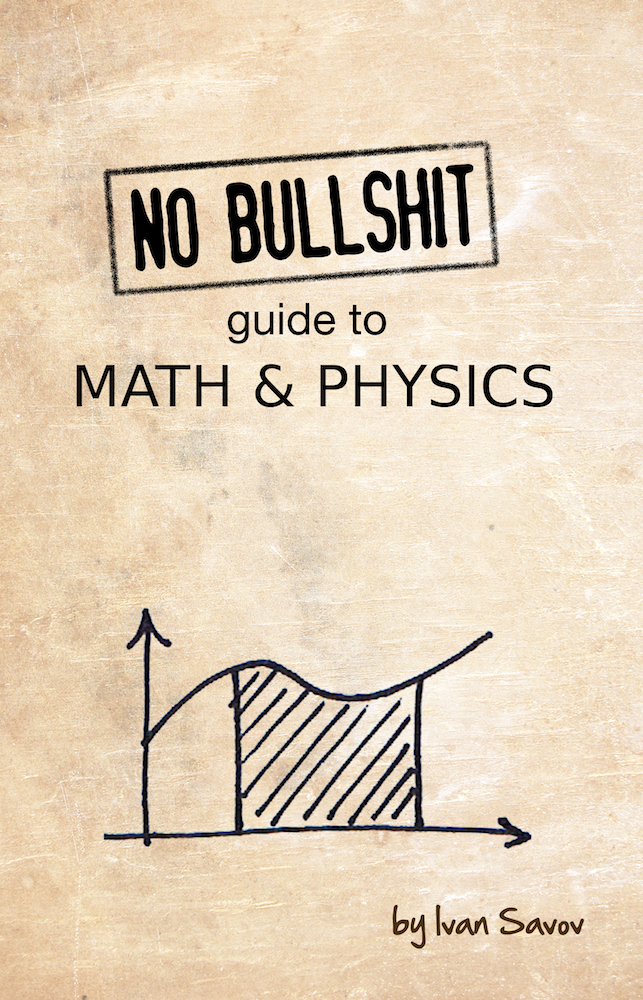
\includegraphics[width=135pt,height=207pt]{figures/cover_v40_noline_lite.png}
%\includegraphics[width=125pt]{/Library/WebServer/Documents/miniref/data/media/physics/mass_spring-highres.png}
\end{wrapfigure}

    This book contains short lessons on math and physics,
    written in a style that is jargon-free and to the point.
    %
    %    The main focus of the book is to show the intricate connections between the concepts of mechanics and calculus.
    %
    Often calculus and mechanics are taught as separate subjects.
    It shouldn't be like that.
    If you learn calculus without mechanics, it will be boring.
    If you learn mechanics without calculus, you won't truly understand what is going on.
    %
    This textbook covers both subjects in an integrated manner.
	%     highlighting the connections between the subjects.
    
Contents:
\begin{itemize}
  \item {\sc high school math}%: (40pp) %Review of algebra, functions and trigonometry.
  \item {\sc vectors}%: (20pp) 
  \item {\sc mechanics} 
  \item {\sc differential calculus}%: (30pp)
  \item {\sc integral calculus}%: (20pp)
  \item 250+ practice problems %: (20pp)
%  \item {\sc linear algebra}%: (60pp) 
\end{itemize}

\noindent
%Available at the \textbf{McGill bookstore.}}{}
  \hfill {\small   5\textonehalf[in] $\times$ 8\textonehalf[in] $\times$ 445[pages] } 


	%Save yourself some time: instead of reading three books you can read just one.
	%The print version will be available December 1$^{\text{st}}$. 
	%Get in touch with me by email if you want to buy a copy of the book in print or as a PDF. 
	%
	%I will also appreciate it if you send me feedback and comments. 
	%where I post other tutorials like this one.
	%Don't hesitate to get in touch with me if you have any questions or feedback: 
	%. I would also like to hear what you feedback
	%do you like the style of writing?

	%in which all the material that you normally taught in first year science is explained in a concise manner.        

	%
	%If you liked this tutorial you can check out the other ones on \url{http://minireference.com}
	%and order the printed book which has not only formulas but also compact explanations:
	%\url{http://minireference.com/order_book/}.


%
%Also of interest, 

%The coverage of the math and physics topics in this tutorial were not sufficient
%to do justice to the subjects. The goal here is to quickly introduce you to the 
%useful \texttt{SymPy} commands. 
%
%you should consider some of my other tutorials on mechanics
%If you're interested in learning more about calculus and mechanics,
%you should consider the \emph{No bullshit guide to math and physics}---a short textbook like no other.

\noindent
For more information, see the book's website %and find more information on the following website 
at \,  \href{http://minireference.com/}{\texttt{minireference.com}}.

The linear algebra examples presented in Section~\ref{sec:linear_algebra} are 
sourced from the \href{https://gum.co/noBSLA}{\textbf{No bullshit guide to linear algebra}}.
Check out the book if you're taking a linear algebra course of if you're missing the prerequisites 
for learning machine learning, computer graphics, or quantum mechanics.

I'll close on a note for potential readers who suffer from math-phobia.
Both books start with an introductory chapter that reviews all 
high school math concepts needed to make math and physics 
accessible to everyone.
Don't worry, we'll fix this math-phobia thing right up for you;
\textbf{when you've got \texttt{SymPy} skills, math fears \emph{you}!}

To stay informed about upcoming titles,
follow \href{https://twitter.com/minireference}{\texttt{@minireference}} on twitter 
and check out the facebook page at \href{http://fb.me/noBSguide}{\texttt{fb.me/noBSguide}}.
%You're also invited to the \textbf{online office hours} where I'll answer 
%your questions and solve problems from past years' finals\  \   \hfill  \href{http://on.fb.me/1aPxy5w}{\texttt{on.fb.me/1aPxy5w}}
%For comments, feedback, and questions, you can get in touch with me here \hfill  




\end{document}

